\cotefile{7}
\scanpage{61}
\[
H^*((U,X'),F)\simeq H^*(X',\unsure{F_{(U,X')}})
\]
Supposons pour \unsure{simplifier} $X$ affine, \deleted{\unsure{et affine sur $S$}}, donc les $\Delta^{(\nu)}(i)$ affines. \unsure{Supposons} que les $F_{\Delta^{(\nu)}(i)}$ soient \uline{quasi-cohérents}\inserted{\uline{et s'induisent mutuellement}}. Alors \unsure{on trouve donc}
\[
H^q(\widetilde{\Delta_X^{(\nu)}(i)},F)=0\qquad\text{si }q>0
\]
\inserted{$H^0(\widetilde{\Delta_X^{(\nu)}(i)},F)$ pour $i$ variable est un \unsure{syst. proj. strict},}
d'où par les \unsure{arguments à la} M.L.
\[
H^q(\widetilde X^{(\nu+1)},F)
=H^q(\varinjlim_i\widetilde{\Delta_X^{(\nu)}(i)},F)
=\varprojlim_i H^q(\widetilde{\Delta_X^{(\nu)}(i)},F)
\]
donc
\[
\left\{\begin{aligned}
H^q(\widetilde X^{(\nu+1)},F)&=0&&\text{si }q>0\\
H^0(\widetilde X^{(\nu+1)},F)&=\varprojlim_i F(\Delta_X^{(\nu)}(i))
\end{aligned}\right.
\]
et par suite un isom \unsure{can}
\[
\left\{\begin{gathered}
H^*(X_{\mathrm{strat}},F)\simeq
H^*\bigl(\nu\longmapsto F(\underbrace{\unsure{\widehat{X^{(\nu+1)}}_{/\deleted{\Delta}X}}}_{\text{complété formel}})\bigr)\\
\text{si $X$ affine, les $F_{\Delta_X^{(\nu)}(i)}$ quasi-cohérents}\quad
\left(\text{p. ex. }F=\unsure{\mathcal O_{X_{\mathrm{strat}}}}\right)
\end{gathered}\right.
\]
Dans le cas où on suppose seulement que les $F_{\Delta_X^{(\nu)}(i)}$ sont qu. coh.\deleted{\unsure{(quasi-induits\ldots ?)}}\inserted{\uline{et s'induisent mutuellement}}, mais $X$ pas \unsure{néc.} affine, on \unsure{voit} que pour tt entier $\nu$, on a un
\mspage{60}
\scanpage{62}
faisceau
\[
\mathcal F^{(\nu)}:\quad U\longmapsto F(U^{(\nu+1)}/U)=\varprojlim_i F(\Delta_U^{(\nu)}(i))
\]
sur $X_{\mathrm{zar}}$, soit $\mathcal F^{(\nu)}$, et que pour $\nu$ variable, ces faisceaux forment un faisceau cosimplicial sur $X_{\mathrm{zar}}$. Ceci posé, on aura un isom
\[
H^*(X_{\mathrm{strat}},F)\simeq\mathbb H^*(X_{\mathrm{zar}},\underset{\substack{\Vert\\(\nu\mapsto\mathcal F^{(\nu)})}}{\mathcal F^*}),
\]
qui implique une suite spectrale d'hypercoh
\[
\boxed{H^*(X_{\unsure{\mathrm{inf}|\mathrm{strat}}},F)\Longleftarrow
E_2^{pq}=H^p(\deleted{\unsure{F}}\nu\longmapsto H^q(X_{\mathrm{zar}},\mathcal F^{(\nu)}))}
\]
\unsure{généralisant} l'isomorphisme donné plus haut.

\deleted{\unsure{Regardons} le complexe $\mathcal F^*$, prenons pour simplifier $F=\mathcal O_{X_{\mathrm{strat}}}$.}

\margin{\uline{Coh. cristalline}}
6.b \unsure{Lorsqu'on travaille} en cohomologie cristalline, on ne peut (si $X$ n'est pas \unsure{f\textsuperscript{t}} lisse sur $S$) affirmer que $\widetilde X$ couvre l'objet final. Mais supposons que l'on puisse trouver une immersion
\mspage{61}
\scanpage{63}
\diagram{\begin{tikzcd}
X \arrow[r,phantom,"\subset" description] \arrow[d] & Y \arrow[dl] \\
S &
\end{tikzcd}}
avec $Y$ form\textsuperscript{t}. lisse sur $S$ [tjs possible \deleted{loc\textsuperscript{t}. sur $X$}, \unsure{ou} si $S,X$ affines, ou si $X$ est qu. projectif sur $S$ \deleted{\unsure{de t. f.}} admettant \unsure{f. inv.} ample]. Considérons le foncteur sur le site cristallin de $X/S$ ``représenté'' par $(X,Y)$ ; de façon précise, si $Y(i)$ est le $i$ième vois. inf. de $X$ dans $Y$, on trouve que ce foncteur est le faisceau
\[
\widetilde Y=\varinjlim_i\widetilde{Y(i)},
\]
d'autre part l'hyp que $Y$ est \unsure{f\textsuperscript{t}} lisse sur $S$ implique que $\widetilde Y$ couvre le faisceau final. D'où encore
\[
H^*(X_{\mathrm{cris}},F)\Longleftarrow E_2^{pq}=H^p(\nu\longmapsto H^q(\widetilde Y^{\nu+1},F))
\]
\mspage{62}
\scanpage{64}
Supposons donc les $F_{X'}$ qu. coh., \deleted{\unsure{et}}\inserted{et s'induisant bien si $X''\subset X'$.} De plus, supposons d'abord $X$ affine, donc les $Y(i)$ affines. \deleted{\unsure{les $H$}} Comme on a encore
\[
H^*(\widetilde{X'},F)=H^*(X'_{\mathrm{zar}},F_{X'})
\]
on trouve encore $E_2^{pq}=0$ si $\unsure{q}\ne0$ d'où
\[
H^*(X_{\mathrm{cris}},F)\simeq H^*(\nu\longmapsto F(\underbrace{Y^{\nu+1}_{/X}}_{\substack{\text{complété formel,}\\\text{le long de }X}}))
\]
\margin{\deleted{[\illegible{1} \unsure{de $X$} \unsure{$(i)$} \illegible{2} \unsure{!}]}}
Lorsque $X$ n'est pas affine, on introduit encore les faisceaux
\[
\mathcal F^{(\nu)}:\quad U\longmapsto\varprojlim F(U,U(i)^{\nu+1})
\]
sur $X_{\mathrm{zar}}$ [$U(i)$ est le $i$ième voisinage inf de $U$ dans $Y^{\nu+1}$ ; si $V$ est un ouvert de $Y$ induisant $U$, cela revient à prendre
\[
\mathcal F^{(\nu)}(U)=F(\underbrace{\widehat{V^{\nu+1}}_{/U}}_{\substack{\text{complété formel}\\\text{le long de }U}})
\]
];
Pour $\nu$ variable, on trouve un faisceau cosimplicial, \deleted{\unsure{d'un}} noté $\mathcal F^*$, et on trouve
\mspage{63}
\scanpage{65}
\[
H^*(X_{\mathrm{cris}},F)\simeq H^*(X_{\mathrm{zar}},\mathcal F^*)
\]
d'où
\[
H^*(X_{\mathrm{cris}},F)\Longleftarrow H^p(\nu\longmapsto H^q(X,\mathcal F^{(\nu)}))
\]
6.3. \uline{Cas particulier} Supposons que \deleted{\unsure{$X\subset Y$ est}}\inserted{l'on ait $X_0\subset X$} une immersion \uline{nilpotente}, \deleted{\unsure{Alors}} et que $F$ sur $X_{\mathrm{cris}}$ provienne d'un $F_0$ sur $X_{0\,\mathrm{cris}}$ par ``restriction''. Alors $\forall$ entier $\nu$, les complétés formels $Y^{\nu+1}_{/X_0}$ et $Y^{\nu+1}_{/X}$ sont identiques, On trouve donc
\margin{\uline{Application aux}\par\uline{\unsure{stratifications}}\par\uline{canoniques}}
\[
\mathcal F^{(\nu)}\simeq\mathcal F_0^{(\nu)}\quad\uline{\unsure{can.}}\quad\text{sur }X_{\mathrm{zar}}=X_{0\,\mathrm{zar}},
\]
d'où aussitôt
\[
H^*(X_{\mathrm{cris}},F)\xrightarrow{\sim}H^*(X_{0\,\mathrm{cris}},F_0).
\]
Ceci a été établi lorsqu'on peut plonger $X$ globalement dans un $Y$ \unsure{f\textsuperscript{t}} lisse sur $S$, mais \deleted{\unsure{par un rais. local}} utilisant un rec. de $X$ par des ouverts affines, on voit que l'on peut se débarrasser de cette hypothèse.

[Il faudrait regarder si on peut se débarrasser de l'hypothèse type quasi-cohérence faite sur $F$ ....?]
\mspage{64}
\scanpage{66}
Supposons en particulier que $X$ \unsure{soit} \uline{lisse} sur $S$, (donc on peut prendre $Y=X$, mais peu importe...) et $S_0\subset S$ une imm. nilpotente, d'où $X_0=X\times_S S_0\longrightarrow X$ imm. nilpotente. Considérons $X_0$ comme sch \uline{sur $S$} (pas sur $S_0$) pour définir $X_{0\,\mathrm{cris}}$.
On trouve alors
\[
H^*(X_{\mathrm{cris}},\mathcal O_{X_{\mathrm{cris}}})=H^*(X_{0\,\mathrm{cris}},\mathcal O_{X_{0\,\mathrm{cris}}})
\]
\uline{Cette relation prouve que le} 1\textsuperscript{er} \uline{mb ne dépend pas} (mod isom canonique) \uline{de la façon dont on a relevé le schéma lisse} $X_0/S_0$ \uline{en un schéma lisse sur} $S$.
Lorsque $S$ est de car. nulle, on verra que le premier mb est isom\inserted{(can. isom :)} à $H^*(X_{\mathrm{zar}},\Omega^{\boldsymbol\cdot}_{X/S})$, et on aura donc trouvé une définition des \uline{\unsure{stratifications}} \uline{can} \uline{en coh. de De Rham}\inserted{pour un morphisme lisse \deleted{\unsure{$f:X\longrightarrow S$}} \unsure{quasi-proj} $f:X\longrightarrow S$,} sur une base $S$ de car. nulle.
(Même mieux, on \deleted{\unsure{pourra en un}} \unsure{saura} arriver à définir $Rf_*(\Omega^{\boldsymbol\cdot}_{X/S})$ comme un \uline{cristal absolu} sur $S$ .....\inserted{ainsi l'étendre à \uline{tt} voisinage infinitésimal de $S$, pas seulement ceux qui loc. se rétractent sur $S$}).
\mspage{65}
\scanpage{67}
\margin{\uline{Cas de} $\mathcal O_{X_{\mathrm{strat}}}$\par\uline{et} $\mathcal O_{X_{\mathrm{cris}}}$}
6.4. Cas $F=\mathcal O_{X_{\mathrm{strat}}}$ ou $\mathcal O_{X_{\mathrm{cris}}}$. Alors $\mathcal F^*$ est un \uline{Anneau cosimplicial}\inserted{sur $X_{\mathrm{zar}}$}. \deleted{\unsure{Dans l'étude suivante}}
Dans le cas de 6.2. c'est la limite projective des anneaux cosimpliciaux $\mathcal F_{(i)}^*$, où $\mathcal F_{(i)}^*$ est celui attaché à $Y(i)$ (NB. $Y(i)_{\mathrm{zar}}=X_{\mathrm{zar}}$ !). On est donc, pour l'étude de cet \unsure{hypercoh}, ramené essentiellement au \deleted{contexte} \unsure{stratifiant}.

Chaque $\mathcal F^{(\nu)}$\inserted{sur $X_{\mathrm{zar}}$} est une $\mathcal O_{X_{\mathrm{zar}}}$-algèbre en $\nu+1$ façons canoniques, grâce aux $\nu+1$ projections $\mathrm{pr}_i$ ($\unsure{1\le i\le\nu+1}$) de $X^{\nu+1}$ sur $X$ donc $X^{\nu+1}_{/X}$ sur $X$. Si on choisit p.ex. $\mathrm{pr}_1$, \inserted{$\mathcal F^{(\nu)}$ devient pro-quasi-cohérent.}\deleted{les} opérations simpliciales, et par suite ces opérateurs cobords doivent être considérés comme \uline{op. diff. d'ordre infini} : si on tronque les $\mathcal F^{(\unsure{\nu})}$, on trouvera des op. diff ordinaires ..... \uline{C'est via ces complexes de cochaines canoniques} (plutôt que par les complexes de De Rham). \uline{que les complexes}
\mspage{66}
\scanpage{68}
\margin{\deleted{Cas de $S=\operatorname{Spec}\unsure{\mathbf C}$}}
\deleted{6.4. Soit $X$ un espace analytique. On peut \unsure{dé}}
\mspage{67}
\scanpage{69}
\uline{d'op. différentielles s'introduisent dans la théorie de façon vraiment naturelle}.

Analogie avec les cochaines de \unsure{Čech}-Alexander....

\margin{\uline{Cas} $S=\operatorname{Spec}\mathbf C$}
6.5 Supposons $S=\operatorname{Spec}\mathbf C$. Regardons la suite spectrale de cohomologie \unsure{stratifiante}
\[
H^*(X_{\unsure{\mathrm{strat}}},\mathcal O_{X_{\mathrm{strat}}})\Longleftarrow E_2^{pq}
=H^p(\nu\longmapsto H^q(\deleted{\unsure{X}}\underbrace{\mathcal O_{X^{\nu+1}_{/X}}}_{\substack{\text{cohomologie}\\\text{formelle}}}))
\]
Si on suppose pour simplifier $X$ propre, alors les $H^q(\Delta^{(\nu)}(i),\mathcal O_{\Delta^{(\nu)}(i)})$ de dim. finie, alors on trouve par M.L.
\[
H^q(X^{\nu+1}_{/X},\mathcal O_{X^{\nu+1}_{/X}})\simeq\varprojlim_i H^q(\Delta^{(\nu)}(i),\mathcal O_{\Delta^{(\nu)}(i)})
\]
et on peut même écrire
\[
E_2^{pq}=\varprojlim_i H^p(\nu\longmapsto H^q(\Delta^{(\nu)}(i),\mathcal O_{\Delta^{(\nu)}(i)})).
\]
Or, grâce à GAGA, la cohomologie des $\Delta^{(\nu)}(i)$ peut s'interpréter de façon analytique. On trouve ainsi
\[
H^*(X_{\unsure{\mathrm{strat}}},\mathcal O_{X_{\unsure{\mathrm{strat}}}})
\simeq H^*(X^{\mathrm{an}}_{\unsure{\mathrm{str}}},\mathcal O_{X^{\mathrm{an}}_{\unsure{\mathrm{str}}}})
\overset{\mathrm{def}}{=}H^*(X^{\mathrm{an}},\mathcal F_{X^{\mathrm{an}}}^{\mathrm{an}*})
\]
\mspage{68}
\scanpage{70}
où $\mathcal F_X^{\mathrm{an}*}$ se \deleted{\unsure{construit}} définit à partir de $X^{\mathrm{an}}$ \deleted{par}\inserted{de} façon analogue que dans le cas algébrique :
\[
\mathcal F_{X^{\mathrm{an}}}^{\deleted{\unsure{\mathrm{an}}}\mathrm{an}*}
=\mathcal F_{X^{\mathrm{an}}}^*
=\deleted{\unsure{\mathcal F}}\mathcal F_{X^{\mathrm{an}}}^{\nu}
\]
\[
\mathcal F_{X^{\mathrm{an}}}^{\nu}:\quad U\longmapsto\Gamma(U^{\nu+1}_{/U},\mathcal O_{U^{\nu+1}_{/U}})
\]
(où $U$ parcourt les ouverts de $X^{\mathrm{an}}$).

\uline{Conjecture} Pour tout espace analytique $\mathfrak X$, le complexe $\mathcal F_{\mathfrak X}^*$ est une \uline{résolution} du faisceau $\mathbf C_{\mathfrak X}$ (via l'augmentation triviale).
\margin{[Alors pour $X$ prop, on a $H^*(\mathfrak X_{\mathrm{str}},\mathcal O_{\mathfrak X_{\mathrm{str}}})=H^*(\mathfrak X,\mathbf C)$]}
\deleted{\uline{NB} \unsure{Cela} \illegible{9}}
Cela semble plausible, en regardant les ``fibres formelles'' des faisceaux...

\uline{Th} Soit $X$ propre sur $\mathbf C$. Si la conjecture plus haut est vraie pour $X^{\mathrm{an}}$, alors on a un isom can
\[
H^*(X_{\mathrm{strat}},\mathcal O_{X_{\mathrm{strat}}})\simeq H^*(X^{\mathrm{an}},\mathbf C)
\]
\mspage{69}
\scanpage{71}
Supposons $X$ contenu dans un schéma lisse $Y$.
\deleted{la conjecture ci-dessus est vraie pour les $Y(i)^{\mathrm{an}}$ ($Y(i)=$ $i$ième voisinage infinitésimal de $X$ sur $Y$)} alors l'hom. \deleted{\unsure{on a}}\inserted{canonique}
\[
H^*(X_{\mathrm{cris}},\mathcal O_{X_{\mathrm{cris}}})\longrightarrow H^*(X_{\mathrm{strat}},\mathcal O_{X_{\mathrm{strat}}})
\]
est également un isom.

Le premier énoncé résulte de l'isom de comparaison plus haut, et de
\[
H^*(X^{\mathrm{an}},\mathcal F_{X^{\mathrm{an}}}^{\deleted{\unsure{\mathrm{an}}}*})\simeq H^*(X^{\mathrm{an}},\mathbf C).
\]
Pour le deuxième, les développements du n° 2 donnent aussitôt
\[
H^*_{\mathrm{cris}}(X,\mathcal O_{X_{\mathrm{cris}}})=\varprojlim_i H^*_{\mathrm{cris}}(Y(i),\mathcal O_{Y(i)_{\mathrm{cris}}})
\]
Or d'après la première partie, les hom de transition sont des isom, et on gagne.

Cela donne donc des espoirs à la conjecture de l'exposé précédent.

\uline{Pb} Supposons de façon générale $X$ \uuline{plat}\inserted{(loc. de prés. finie)} sur $S$, et $F$\inserted{sur $X_{\mathrm{cris}}$}, satisfaisant aux hyp. habituelles (p.ex. provenant d'un Module qu. coh. stratifié) À prouver qu'alors
\[
H^*(X_{\mathrm{cris}},\deleted{\mathcal O_{X_{\mathrm{cris}}}}F)\xrightarrow{\sim}H^*(X_{\mathrm{strat}},F\ (\text{site stratifié})).
\]
\mspage{70}
\scanpage{72}
C'est \unsure{aussi} équivalent au pb suivant : si $X$ est comme dessus, et $X_0-X$ une imm. \uline{nilp. loc.}, $\unsure{Y|X}$ de prés. finie sur $S$, a-t-on
\[
H^*(X_{\unsure{\mathrm{strat}}},F)\xrightarrow{\sim}H^*(X_{0\,\mathrm{str.}},F)
\]
[De plus, on peut supposer $S,X,X_0$ affines].

\uline{Remarque} Si $S=\operatorname{Spec}k$, $k$ corps valué complet non archimédien, il y a lieu de \deleted{faire} se \deleted{\unsure{demander}}\inserted{poser la question de la validité de la} conjecture \unsure{plus} ci-dessus, pour les \deleted{espaces \uline{rigide-analytiques} de Tate (au sens \unsure{strict}, [\unsure{et rigides}, --- mais en \unsure{considérant} les} espaces analytiques \deleted{\unsure{ordinaires}} ``flasques'' sur $k$ ].
\deleted{Cela expliquerait} Mais cela n'aurait pas d'implications globales si remarquables ....
\mspage{71}
\cotefile{8}
\scanpage{1}
\figure{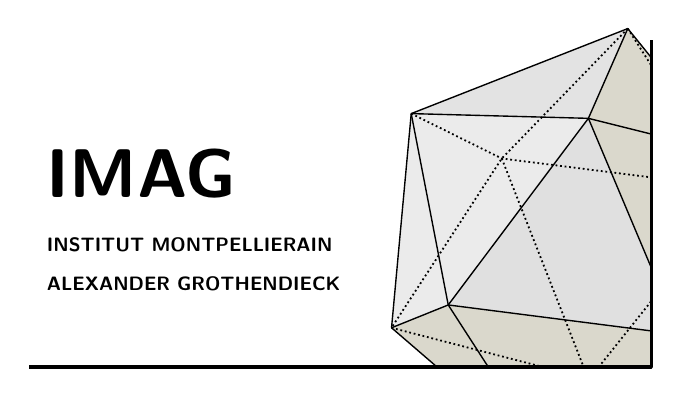
\begin{tikzpicture}[x=1mm,y=1mm,line join=round]
\node[anchor=west,font=\sffamily\bfseries\fontsize{33}{35}\selectfont] at (2,27) {IMAG};
\node[anchor=west,font=\sffamily\bfseries\fontsize{6.7}{8}\selectfont] at (2,18) {INSTITUT MONTPELLIERAIN};
\node[anchor=west,font=\sffamily\bfseries\fontsize{6.7}{8}\selectfont] at (2,13) {ALEXANDER GROTHENDIECK};
\fill[gray!22] (49.5,34.6)--(77,45.4)--(72,34)--cycle;
\fill[gray!16] (49.5,34.6)--(72,34)--(54.2,10.3)--cycle;
\fill[gray!24] (54.2,10.3)--(72,34)--(80,15)--(80,7)--cycle;
\fill[yellow!15!gray!40] (77,45.4)--(80,41.7)--(80,15)--(72,34)--cycle;
\fill[yellow!15!gray!40] (47,7.4)--(54.2,10.3)--(80,7)--(80,2.4)--(52.8,2.4)--cycle;
\fill[gray!16] (49.5,34.6)--(54.2,10.3)--(47,7.4)--cycle;
\draw[line width=.5pt] (47,7.4)--(49.5,34.6)--(77,45.4)--(80,41.7);
\draw[line width=.5pt] (49.5,34.6)--(72,34)--(80,32);
\draw[line width=.5pt] (77,45.4)--(72,34)--(80,15);
\draw[line width=.5pt] (47,7.4)--(54.2,10.3)--(72,34);
\draw[line width=.5pt] (49.5,34.6)--(54.2,10.3)--(59.3,2.4);
\draw[line width=.5pt] (54.2,10.3)--(80,7);
\draw[line width=.5pt] (47,7.4)--(52.8,2.4);
\draw[densely dotted,line width=.65pt] (77,45.4)--(61,28.9)--(47,7.4);
\draw[densely dotted,line width=.65pt] (49.5,34.6)--(61,28.9)--(80,26.5);
\draw[densely dotted,line width=.65pt] (61,28.9)--(71.4,2.4);
\draw[densely dotted,line width=.65pt] (47,7.4)--(66.3,2.4);
\draw[densely dotted,line width=.65pt] (73.3,2.4)--(80,10.8);
\draw[densely dotted,line width=.65pt] (77,45.4)--(80,40.7);
\draw[line width=1.2pt] (1,2.4)--(80,2.4)--(80,44);
\end{tikzpicture}}
\scanpage{2}
\[
\boxed{\begin{array}{l}C:\omega\longrightarrow\omega^{(p)}\\ \Pi:\mathfrak g^{(p)}\mathbin{-}\mathfrak g\end{array}}
\]
\diagram{\begin{tikzcd}[column sep=small]
& \unsure{\check{\ell}_{\bullet}^{G^*}=Q}\arrow[dl,"(1)"'] & \\
\ell_{\bullet}^{\unsure{G|C}}[-1]\arrow[rr] & & \Delta^*(\unsure{G|Q})\arrow[ul]
\end{tikzcd}}
\margin{$\unsure{P}\;''$}
\[
\simeq
\]
\deleted{$\unsure{\omega^{(p)}}$}
\diagram{\begin{tikzcd}[column sep=small]
& [\omega\xrightarrow{C}\omega^{(p)}]\arrow[dl,"(\mathrm{id},0)"',"\deg 1"] & \\
[\omega^{(p)}\xrightarrow{0}\omega]\arrow[rr,"(\mathrm{id},C)"'] & & [\omega^{(p)}\xrightarrow{0}\omega^{(p)}]\arrow[ul,"(0,\mathrm{id})"']
\end{tikzcd}}
\deleted{$\unsure{\ne}$}
\diagram{\begin{tikzcd}[column sep=small]
& \deleted{\unsure{\check{\ell}}}\,\unsure{\ell_{\bullet}^{G}[1]^{(p)}=P^{(p)}}\arrow[dl,"(1)"'] & \\
\unsure{\check{\ell}_{\bullet}^{G^*\,(p)}}\arrow[rr] & & \Delta^*(G)\arrow[ul]\\
\unsure{Q^{(p)}}\arrow[u,equal] & &
\end{tikzcd}}
\[
\simeq
\]
\diagram{\begin{tikzcd}[column sep=small]
& [\omega^{(p^2)}\xrightarrow{\unsure{0}}\omega^{(p)}]\arrow[dl,"(\mathrm{id},0)"',"\deg 1"] & \\
[\omega^{(p)}\xrightarrow{C^{(p)}}\omega^{(p^2)}]\arrow[rr,"(\mathrm{id},0)"'] & & [\omega^{(p)}\xrightarrow{0}\omega^{(p)}]\arrow[ul,"(C,\mathrm{id})"']
\end{tikzcd}}
\margin{\diagram{\begin{tikzcd}S_{\mathrm{cris}}\arrow[d,"\varphi"']\\S_{\mathrm{zar}}\arrow[u,bend right=40,"\varepsilon"']\end{tikzcd}}
$\varphi\varepsilon=\deleted{\unsure{f}}F_S$\\
frobenius absolu}

$\Delta^*(G)$ complexe cristallin avec $F,V$, filtration à facteurs
\[
\boxed{\varphi^*(Q),\varphi^*(P)}
\]
$+$ filtration sur $\Delta^*(G)=\varepsilon^*(\Delta(G))$ à facteurs $P,Q$.

\deleted{$\unsure{\Delta}$}
\diagram{\begin{tikzcd}
\varphi^*(\omega)\arrow[r,"\varphi^*(C)"]\arrow[d,equal]&\varphi^{\unsure{*}}(\omega^p)\arrow[d,equal]\\
D^*(G)&D^*(G)^{(p)}\arrow[l,bend left=20,"F=0"]
\end{tikzcd}}
\figure{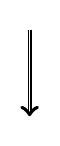
\begin{tikzpicture}\draw[->,double] (0,1.1)--(0,0);\end{tikzpicture}}
\diagram{\begin{tikzcd}
M\arrow[r,bend left=12,"V"]&M^{(p)}\arrow[l,bend left=12,"F"]\arrow[d,"i"']\\
&[\varepsilon^*(M)\xrightarrow{0}\varepsilon^*(M)]
\end{tikzcd}}
\[
M=D^*(G)
\]
\deleted{$\unsure{\Delta^*(G)=\varepsilon^*(M)^0}$}
\[
\Delta^*(G)=[\varepsilon^*(M)\xrightarrow{0}\varepsilon^*(M)]
=\varepsilon^*[M\longrightarrow M]
\]
\diagram{\begin{tikzcd}[column sep=small]
& [M^{\deleted{\unsure{(p)}}}\xrightarrow{V}M^{(p)}]\arrow[dl,"(\mathrm{id},0)"',"(\deg 1)"]&\\
[M^{(p)}\xrightarrow{F}M^{\deleted{\unsure{(p)}}}]\arrow[rr,"(\mathrm{id},0)"']&&\Delta^*(G)=[M\xrightarrow{0}M]\arrow[ul,"(\unsure{V},\mathrm{id})"']
\end{tikzcd}}
\[
\unsure{\cdot}\mathbin{-}_{F}M^{(p)}\mathbin{-}M\mathbin{-}_{V}M^{(p)}\longrightarrow
\]
\mspage{1}
\scanpage{3}
132.

\uline{\S24. Explicit description of pseudo-rational double points.}

Let $R$ be a two-dimensional normal local ring of multiplicity two having a pseudo-rational singularity. Since $\lambda(m^2)=4$ (Corollary 23.3) every minimal basis of the maximal ideal $m$ of $R$ consists of three elements. We shall classify $R$ by studying its behaviour under successive quadratic transformations, and by relating this behaviour to certain conditions involving, more or less explicitly, a suitable basis $\{x,y,z\}$ of $m$. We also prove converse statements of the type: ``If $R$ is any local ring, with maximal ideal $m$ generated by elements $x,y,z$ satisfying $\ldots$ then $R$ is a two-dimensional normal local ring having a (pseudo-) rational singularity.'' In other \textbf{words} the conditions to be introduced \uline{characterize} (pseudo-) rational ``double points.''

Basically, the idea is to take a two-dimensional local ring of multiplicity two whose maximal ideal is generated by three elements, say $x,y,z$, to subject this ring to a succession of quadratic transformations, and to see what conditions on $x,y,z$, guarantee that the resulting rings are all \uline{normal} (cf. Proposition 23.5). This approach involves a detailed and rather tedious examination of numerous cases. For orientation, the reader may analyse a ring of the form
\[
k[[X,Y,Z]]/(Z^2-f(X,Y))
\]
($k$-a field) from this point of view.
\[
*\qquad\qquad *\qquad\qquad *
\]
\mspage{2}
\scanpage{4}
\deleted{\unsure{Schémas-gr.}} \inserted{finis} \unsure{loc.} libres annulés par $p$ en car $p$.

a) Cristal (loc. libre de \unsure{t. fini} ?) $\mathcal M$ sur $S_{\mathrm{cris}}/\mathbb F_p$

avec
\diagram{\begin{tikzcd}\mathcal M^{(p)}\arrow[r,bend left=12,"F_{\mathcal M}"]&\mathcal M\arrow[l,bend left=12,"V_{\mathcal M}"]\end{tikzcd}}
satisfaisant $FV=VF=p$.

On en déduit complexe cristallin parfait, amplitude parfaite $\subset[0,1]$
\[
\mathbb\Delta^*=\mathbb\Delta^*(\mathcal M),\qquad \mathcal H^0(\mathbb\Delta^*)\simeq\mathcal H^1(\mathbb\Delta^*)\simeq\mathcal M
\]
avec $F_{\mathbb\Delta^*},V_{\mathbb\Delta^*}$ satisfaisant $F_{\mathbb\Delta^*}V_{\mathbb\Delta^*}=0$, $V_{\mathbb\Delta^*}F_{\mathbb\Delta^*}=0$
et triangles exacts
\[
(\mathrm I)_{\mathrm{cris}}
\]
\diagram{\begin{tikzcd}[column sep=small]
&[\mathcal M\xrightarrow{V}\mathcal M^{(p)}]\arrow[dl,"\partial_{\mathrm I}"',"1"]&\\
[\mathcal M^{(p)}\xrightarrow{F}\mathcal M]\arrow[rr,"i_{\mathrm I}"]&&\mathbb\Delta^{*\,(p)}\arrow[ul,"\pi_{\mathrm I}"']
\end{tikzcd}}
\margin{$\simeq\varphi^*(\Delta^*)$\\$(\Delta^*=\varepsilon^*(\mathbb\Delta^*))$}
\[
(\mathrm {II})_{\mathrm{cris}}
\]
\diagram{\begin{tikzcd}[column sep=small]
&[\mathcal M^{(p)}\xrightarrow{F}\mathcal M]\arrow[dl,"\partial_{\mathrm {II}}"',"1"]&\\
[\mathcal M\xrightarrow{V}\mathcal M^{(p)}]\arrow[rr,"i_{\mathrm {II}}"]&&\mathbb\Delta^*\arrow[ul,"\pi_{\mathrm {II}}"']
\end{tikzcd}}
\margin{NB les complexes
\[
\check L_{\bullet}(\mathcal M)=[\mathcal M^{(p)}\xrightarrow{F}\mathcal M][1]
\]
\[
L'_{\bullet}(\mathcal M)=(\mathcal M\xrightarrow{V}\mathcal M^{(p)})^{\unsure{\vee}}
\]
\[
\mathbb\Delta^*(\mathcal M)
\]
sont des $(F,V)$-complexes, et ces triangles écrits $(\mathrm I)$ $(\mathrm {II})$ sont compatibles avec $(F,V)$-structure.
\diagram{\begin{tikzcd}\unsure{F\ \mathrm{nul}}&\check L_{\bullet}(\mathcal M)\arrow[l]\\\unsure{V\ \mathrm{nul}}&L'_{\bullet}(\mathcal M)\arrow[l]\end{tikzcd}}}
\deleted{\unsure{additif} \unsure{$(\mathcal O_S)$-} \unsure{différentiels}}

b) Complexes parfaits $\ell_{\bullet},\ell'_{\bullet}$ sur $S_{\mathrm{zar}}$, d'amplitude parfaite $\subset[-1,0]$, \deleted{\unsure{et des complexes} \unsure{cristallins}} \inserted{triangle exact} $(\mathrm {III})$:
\diagram{\begin{tikzcd}[column sep=small]
&\check\ell'_{\bullet}\arrow[dl,"\partial_0"']&\\
\ell_{\bullet}[-1]\arrow[rr,"i_0"]&&\Delta^*\arrow[ul,"\pi_0"']\arrow[dr,equal,"\mathrm{dfn}"]&\\
&&&\varepsilon^*(\mathbb\Delta^*)
\end{tikzcd}}
\[
\varphi^*(\ell_{\bullet}[-1])\overset{\unsure{\alpha}}\simeq[\mathcal M^{(p)}\xrightarrow{F}\mathcal M]
\]
\[
\varphi^*(\check\ell'_{\bullet})\simeq[\mathcal M\xrightarrow{V}\mathcal M^{(p)}]
\]
fournissant un \deleted{\unsure{morph.}} \inserted{isom} de $(\mathrm I_{\mathrm{cris}})$ avec $\varphi^*(\mathrm {III})$

\deleted{\unsure{[}} [d'où, posant $M=\varepsilon^*(\mathcal M)$ loc libre sur $S_{\mathrm{zar}}$, avec connexion à courbure nulle,
\[
\ell_{\bullet}[-1]^{(p)}\simeq[M^{(p)}\xrightarrow{F_M}\uline{M}]
\]
\[
\check\ell'_{\bullet}\deleted{\unsure{\varepsilon}}{}^{(p)}\simeq[M\xrightarrow{V_M}M^{(p)}]\qquad !\ ]
\]
\margin{comp. avec connexions}

\uline{Compatibilité}: \inserted{Posons}
\[
\left\{\begin{aligned}
\pi_0\varepsilon^*(i_{\mathrm {II}})&\mathrel{\text{``$=$''}}F_{\check\ell'_{\bullet}}={}^tV_{\ell'_{\bullet}}\\
\varepsilon^*(\pi_{\mathrm {II}})i_0&\mathrel{\text{``$=$''}}V_{\ell_{\bullet}}[-1]
\end{aligned}\right.
\]
\mspage{3}
\scanpage{5}
$G/S$ \unsure{gpe} fini loc. libre annulé par $p$, en car. $p>0$ ;

On lui associe (conjecturalement)

\deleted{
a) $\mathbb D^*(G)$ Module (de présentation finie ?) \inserted{loc. libre de type fini ?} sur $S_{\mathrm{cris}}$
(topos cristallin de \unsure{Berthelot} de $S$ sur $\mathbb F_p$)
\margin{[\unsure{fonctoriel} en $G$, \uline{donc}:]}

b) homomorphismes
\diagram{\begin{tikzcd}\mathbb D^*(G)^{(p)}\arrow[r,bend left=12,"F"]&\mathbb D^*(G)\arrow[l,bend left=12,"V"]\end{tikzcd}}
avec $FV=0$, $VF=0$

c) des complexes $\ell_{\bullet}^G$ et $\ell_{\bullet}^{G^*}$ sur $S$, parfaits d'amplitude parfaite dans $[-1,0]$, et un hom \deleted{$\unsure{\alpha}$}
\[
(\ell_{\bullet}^{G^*})^\vee\xrightarrow{\pi}\ell_{\bullet}^G
\]
i.e. un hom
\[
\mathcal O_S\longrightarrow\ell_{\bullet}^{G^*}\overset L\otimes\ell_{\bullet}^G
\]
\margin{\diagram{\begin{tikzcd}S_{\mathrm{cris}}\arrow[d,"\varphi"']\\S_{\mathrm{zar}}\arrow[u,bend right=40,"\varepsilon"']\end{tikzcd}}}

d) \deleted{\unsure{Deux}} \inserted{Un} triangles exacts sur $S_{\mathrm{cris}}$
\diagram{\begin{tikzcd}[column sep=small]
&\varphi^*(\ell_{\bullet}^{\unsure{G}})^{\deleted{\unsure{*}}}[-1]\arrow[dl,"\partial\deleted{\unsure{\varphi^*(\pi)}}"']&\\
\varphi^*(\check\ell_{\bullet}^{G^*})\deleted{\unsure{[1]}}\arrow[rr]&&\mathbb\Delta^*_{\mathrm{cris}}(G)\arrow[ul]
\end{tikzcd}}
\margin{[NB $\varphi^*(\pi):\mathcal O_{S_{\mathrm{cris}}}\xrightarrow{2}\varphi^*(\check\ell_{\bullet}^{\unsure{G^*}}\otimes\check\ell_{\bullet}^{G^*})$]}
(qui détermine donc $\mathbb\Delta^*_{\mathrm{cris}}(G)$ : isom (non unique près)) et des isom
\[
\mathcal H^0(\mathbb\Delta^*_{\mathrm{cris}}(G))\simeq\mathbb D^*(G),\quad
\mathcal H^1(\mathbb\Delta^*_{\mathrm{cris}}(G))\simeq\mathbb D^*(G)
\]
(d'où par application de $\varepsilon^*$ un triangle
\diagram{\begin{tikzcd}[column sep=small]
&(\ell_{\bullet}^{G})^{(p)}[-1]\arrow[dl,"\varepsilon^*(\partial)\deleted{\unsure{\pi}}"']&\\
(\check\ell_{\bullet}^{G^*})^{(p)}\arrow[rr,dash]&&\Delta^*(G)\arrow[ul]
\end{tikzcd}}
\margin{$\Delta^*(G)=\varepsilon^*(\mathbb\Delta^*_{\mathrm{cris}}(G))$}
}

e) Un triangle exact
\mspage{4}
\scanpage{6}
\[
\begin{array}{ll}
V_{\ell_{\bullet}}:\ell_{\bullet}\mathbin{-}\ell_{\bullet}^{(p)}&F_{\ell_{\bullet}}=0:\ell_{\bullet}^{(p)}\mathbin{-}\ell_{\bullet}\\
V_{\ell'_{\bullet}}:\ell'_{\bullet}\mathbin{-}\ell_{\bullet}'{}^{(p)}&F_{\ell'_{\bullet}}=0:\ell_{\bullet}'{}^{(p)}\mathbin{-}\ell'_{\bullet}
\end{array}
\]
1) le triangle $(\mathrm {III})$ est compatible avec $(F,V)$-structure : \uuline{\unsure{autos}} !

2) L'isom $\varphi^*(\mathrm {III})=\mathrm I$ compatible avec $(F-V)$-structures.

\deleted{\unsure{un}}\qquad\deleted{$\unsure{\Delta^{*\,(p)}\longrightarrow\Delta^*}$}

\uline{1)}
\diagram{\begin{tikzcd}
\Delta^{*p}\arrow[rr,"F_{\Delta^*}"]\arrow[dr,"\deleted{\unsure{*}}\pi_0^{(p)}"']&&\Delta^*\\
&\check\ell'{}^{(p)}\arrow[ur,"\varepsilon^*(i_{\mathrm {II}})"']&
\end{tikzcd}}
\[
\begin{gathered}\pi_0^{(p)}\\\Vert\\\varepsilon^*(\varphi^*(\pi_0))\\\Vert\\\varepsilon^*(\pi_{\mathrm I})\end{gathered}
\]
\margin{impl que $i_0$ comp. avec $F$}
\diagram{\begin{tikzcd}
\Delta^*\arrow[rr,dash,"V_{\Delta^*}"]\arrow[dr,"\varepsilon^*(\pi_{\mathrm {II}})"']&&\Delta^{*\,(p)}\\
&\ell_{\bullet}^{\unsure{(p)}}[-1]\arrow[ur,"i_0^{(p)}=\varepsilon^*\varphi^*(i_0)=\varepsilon^*(i_{\mathrm I})"']&
\end{tikzcd}}
\margin{impl que $\pi_0$ compatible avec $V$}

$i_0$ compatible avec $V$:
\diagram{\begin{tikzcd}
\ell_{\bullet}[-1]\arrow[r,"i_0"]&\Delta^*\arrow[d,"V_{\Delta^*}"]\arrow[dr,"\varepsilon^*(\pi_{\mathrm {II}})"]&\\
\ell_{\bullet}[-1]^{(p)}\arrow[r,dash,"i_0^{(p)}"]&\Delta^{*\,(p)}&\ell_{\bullet}^{(p)}[-1]\arrow[l,"i_0^{(p)}"]
\end{tikzcd}}
\[
\varepsilon^*(\pi_{\mathrm {II}})i_0\ne V_{\ell_{\bullet}}[-1]
\]
\margin{OK}

on voit de $=$ que $\pi_0$ compatible avec $F$.

$\partial_0$ compatible avec $F$
\diagram{\begin{tikzcd}
\check\ell'_{\bullet}{}^{(p)}\arrow[r,"\pi_0\varepsilon^*(i_{\mathrm {II}})"]\arrow[d,"\partial_0^{(p)}"']&\check\ell'_{\bullet}\arrow[d,"\partial_0"]\\
\ell_{\bullet}[-1]^{(p)}\arrow[r,"0"]&\ell_{\bullet}[-1]
\end{tikzcd}}
\margin{$\unsure{1}$\qquad $\underbrace{\partial_0\pi_0}\varepsilon^*(i_{\mathrm {II}})=0$}

on voit de $=$ $\partial_0$ compatible avec $V$.

2) A prouver que
\[
\left\{\begin{aligned}
\varphi^*(V_{\ell_{\bullet}}[-1])&=V_{[\mathcal M^{p}\xrightarrow{F}\mathcal M]}\\
\varphi^*(F_{\check\ell'_{\bullet}}[-1])&=F_{[\mathcal M\xrightarrow{V}\mathcal M^p]}
\end{aligned}\right.
\]
\[
\varphi^*(V_{\ell_{\bullet}}[-1])=\varphi^*(\varepsilon^*(\pi_{\mathrm {II}})i_0)
=\varphi^*\varepsilon^*(\pi_{\mathrm {II}})\varphi^*(i_0)
=\big|\pi_{\mathrm {II}}^{(p)}i_{\mathrm I}=V_{[\mathcal M^{\unsure{(p)}}\mathbin{-}\mathcal M]}\big)
\]
et l'autre relation se prouve de $=$ !!
\mspage{5}
\scanpage{7}
\mspage{35}
\deleted{
Alors puisque (5.1)(iii) est vrai pour $(g,\bar f,\bar G)$ et pour $(g',\pi,\bar G)$, les faisceaux $\deleted{\unsure{(}}R^q\bar f'_*\deleted{\unsure{)}}\inserted{(}\bar g^*\bar G\inserted{)}\simeq\unsure{g}^*(R^q\bar f_*\deleted{\unsure{)}}\inserted{(}\bar G\inserted{)})$ et $\deleted{\unsure{(}}R^q\pi'_*\deleted{\unsure{)}}\inserted{(}\bar g^*\bar G\inserted{)}\simeq g'^*(R^q\pi_*\deleted{\unsure{)}}\inserted{(}\bar G\inserted{)})$ sont nuls pour $q>0$. Il \deleted{s'ensuite}\inserted{résulte} de la suite spectrale de Leray
\[
E_2^{p,q}=\deleted{\unsure{(}}R^pf'_*\deleted{\unsure{)}}\inserted{(}(\deleted{\unsure{(}}R^q\pi'_*\deleted{\unsure{)}}\inserted{(}\bar g^*\bar G\inserted{)})\Longrightarrow\deleted{\unsure{(}}R^n\bar f'_*\deleted{\unsure{)}}\inserted{(}\bar G\inserted{)}
\]
qu'on a aussi $\deleted{\unsure{(}}R^pf'_*\deleted{\unsure{)}}\inserted{(}\pi'_*\bar g^*\bar G\inserted{)}=0$ pour $q>0$.

Or $\pi'_*\bar g^*\bar G\simeq g'^*(\pi_*\bar G)$, d'où $\deleted{\unsure{(}}R^pf'_*\deleted{\unsure{)}}\inserted{(}g'^*(\pi_*\bar G)\inserted{)}=0$ pour $q>0$. L'injection $\pi_*\bar F\longrightarrow\pi_*\bar G$ est donc un \deleted{\unsure{bon}} effacement des foncteurs $(R^pf'_*)g'^*$ dans la catégorie des faisceaux de torsion\inserted{(IX.1.2.(v))}, d'où le résultat.
}
\margin{$]\ ]$}

\uline{Lemme (8.4):} Il suffit de vérifier le théorème (5.1)(i) (resp. (i) et (ii), resp. (iii) ) pour $(g,f,F)$ avec $f$ \uline{projectif.}

Démonstration. Supposons le théorème (5.1)(i) (resp. $\ldots$) vrai chaque fois que $f$ est projectif, et soit $(g,f,F)$ arbitraire. D'après (6.5) avec $P$ la propriété vide, on peut supposer $S$ strictement local et $g:s_o\longrightarrow S$ l'inclusion du point fermé. Considérons la famille $\unsure{\mathfrak F|\mathcal F}$ des sous-préschémas fermés $h:Y\longrightarrow X$ tels que $Y$ contienne la fibre fermée $X_o$ de $X/S$ et tels que pour chaque $F$ et pour chaque $q$ \deleted{Applicable}\inserted{pertinent,} le morphisme
\[
H^q(X,F)\longrightarrow H^q(X,h_*h^*F)
\]
\mspage{6}
\scanpage{8}
\diagram{\begin{tikzcd}
M\arrow[r,"V"]\arrow[d,"V"]&M^{(p)}\arrow[d,"V^{(p)}"]\\
M^{(p)}\arrow[r,"V^{(p)}"]\arrow[u,bend left=45,"F"]&M^{(p^2)}\arrow[u,bend left=35,"F^{(p)}"]
\end{tikzcd}}
\[
\unsure{V^\vee}\quad F
\]
\[
M
\]
$(\mathrm I)$
\diagram{\begin{tikzcd}&B\arrow[dl,"\partial_{\mathrm I}"']&\\A\arrow[rr,"i_{\mathrm I}"]&&\unsure{\mathfrak X|\mathcal X}^{p}\arrow[ul,"\pi_{\mathrm I}"']\end{tikzcd}}
$(\mathrm {II})$
\diagram{\begin{tikzcd}&A\arrow[dl,"\partial_{\mathrm {II}}"']&\\B\arrow[rr,dash,"i_{\mathrm {II}}"]&&\mathfrak X\arrow[ul,"\pi_{\mathrm {II}}"']\end{tikzcd}}
$(\mathrm {II}^{(p)})$
\diagram{\begin{tikzcd}&A^p\arrow[dl,"\partial_{\mathrm {II}}^{(p)}"']&\\B^p\arrow[rr,"i_{\mathrm {II}}^{(p)}"']&&\mathfrak X^p\arrow[ul,"\pi_{\mathrm {II}}^{(p)}"']\end{tikzcd}}
\[
\boxed{\begin{array}{ll}
\unsure{i_{\mathrm {II}}}\pi_{\mathrm I}:&\mathfrak X^p\overset{F_{\mathfrak X}}{\mathbin{-}}\mathfrak X\\
i_{\mathrm I}\pi_{\mathrm {II}}:&\mathfrak X\xrightarrow{V_{\mathfrak X}}\mathfrak X^p
\end{array}}
\]
\[
\boxed{\left\{\begin{array}{ll}
\partial_{\mathrm I}\partial_{\mathrm {II}}:&A^{\deleted{\unsure{a}}}\xrightarrow{2}A\quad\text{nul?}\\
\partial_{\mathrm {II}}\partial_{\mathrm I}:&B^{\deleted{\unsure{a}}}\xrightarrow{2}B\quad\text{nul?}\\
\pi_{\mathrm {II}}^{(p)}i_{\mathrm I}:&A\xrightarrow{V_A}A^{(p)}\\
\pi_{\mathrm I}\deleted{\unsure{\mu}}\,i_{\mathrm {II}}^{(p)}:&B^{(p)}\overset{F_B}{\mathbin{-}}B^{\deleted{\unsure{(p)}}}
\end{array}\right.}
\]
\figure{\begin{tikzpicture}[x=1cm,y=1cm]
\draw (0,3) ellipse (.65 and .27);\node at (0,3){nul?};
\draw (0,2.3) ellipse (.65 and .27);\node at (0,2.3){nul?};
\draw[->] (-1.8,3.7)--(-3.9,3.6);
\draw[->] (-3.5,1)--(-3.7,3.5);
\draw[->] (-3.4,.8)--(-1.9,.9);
\draw[->] (-3.8,-2.3) to[bend left=30] (-3.6,.9);
\draw[->] (-3.95,-2.2) to[bend left=30] (-3.65,1.15);
\draw (-3.85,.9)--(-3.6,1.2)--(-2.9,.9);
\node at (-3.8,.35){$\unsure{\mu}$};
\end{tikzpicture}}

$\varphi^*(\mathrm {III})\simeq(\mathrm I^{\unsure{?}})$
\diagram{\begin{tikzcd}
&\varphi^*(\unsure{b})\arrow[dl,"(\partial_{\mathrm I}\simeq\varphi^*(\partial_0))"']&\\
\varphi^*(a)\unsure{A}\arrow[rr,"(i_{\mathrm I}=\varphi^*(i_0))"]&&\mathfrak X^p\arrow[ul,"(\pi_{\mathrm I}\simeq\varphi^*(\pi_0))"']
\end{tikzcd}}
$\mathrm {III}$
\diagram{\begin{tikzcd}&b\arrow[dl,"\partial_0"']&\\a\arrow[rr,dash,"i_0"]&&\mathfrak X\arrow[ul,"\pi_0"']\end{tikzcd}}
\figure{\begin{tikzpicture}\draw (0,1.5)--(7,1.8);\draw(0,0)--(5.4,.2);\draw(4.8,0)--(4.8,1.7);\end{tikzpicture}}

\diagram{\begin{tikzcd}[column sep=small,row sep=small]
&0\arrow[r,dash]\arrow[d,dash]&M\arrow[r]\arrow[d]&M^p\arrow[r,dash]\arrow[d]&\unsure{\cdot}\\
&M^p\arrow[r,dash]\arrow[d]&M\arrow[r,dash]\arrow[d,dash]&0\arrow[r,dash]\arrow[d,dash]&{}\\
M\arrow[r,dash]&M^p\arrow[r,dash]&\unsure{0}\arrow[r,dash]&\unsure{\cdot}&
\end{tikzcd}}
$\varepsilon^*(\mathrm I)\simeq\mathrm {III}^{(p)}$
\diagram{\begin{tikzcd}&b^p\arrow[dl,"\partial_0^{(p)}"']&\\a^p\arrow[rr,dash,"i_0^{(p)}"]&&X^p\arrow[ul,"\pi_0^{(p)}"']\end{tikzcd}}
$\varepsilon^*(\mathrm {II}):$
\diagram{\begin{tikzcd}&a^p\arrow[dl,"\varepsilon^*(\partial_{\mathrm {II}})"']&\\b^p\arrow[rr,"\varepsilon^*(i_{\mathrm {II}})"']&&X\arrow[ul,"\varepsilon^*(\pi_{\mathrm {II}})"']\end{tikzcd}}
\margin{$\left.\begin{array}{c}\phantom{a}\\\phantom{a}\\\phantom{a}\end{array}\right\}$ triangles compatibles avec $F-V$ structures}

\deleted{$\unsure{\partial_0\varepsilon^*}$}
\[
\boxed{\left\{\begin{array}{ll}
\pi_0\varepsilon^*(i_{\mathrm {II}}):&b^{(p)}\xrightarrow{F_b}b\\\hline
\deleted{\unsure{\partial}}\varepsilon^*(\pi_{\mathrm {II}})i_0:&a\xrightarrow{V_a}a^{(p)}
\end{array}\right.}
\]
\figure{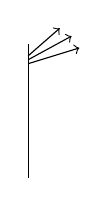
\begin{tikzpicture}\draw (0,0)--(0,1.7);\draw[->](0,1.55)--(.4,1.9);\draw[->](0,1.5)--(.55,1.8);\draw[->](0,1.45)--(.65,1.65);\end{tikzpicture}}
\diagram{\begin{tikzcd}\mathfrak X^p\arrow[r,dash]&B\arrow[r,dash]&\mathfrak X\end{tikzcd}}
\diagram{\begin{tikzcd}\mathfrak X\arrow[r,dash]&A\arrow[r,dash]&\mathfrak X^{(p)}\end{tikzcd}}
\diagram{\begin{tikzcd}X^{(p)}\arrow[r]&b^{(p)}\arrow[r,dash]&X\end{tikzcd}}
\diagram{\begin{tikzcd}X\arrow[r,dash]&a^{(p)}\arrow[r,dash]&X^{(p)}\end{tikzcd}}
\mspage{7}
\scanpage{9}
\mspage{37.1}
\deleted{
où les flèches verticales sont injectives (6.6). Il s'ensuit\deleted{e} que l'élément $\alpha_o\in H^0(X_o,F_o)$ se relève à $H^0(X,F)$ si et seulement si son image $\inserted{\beta_o}$ dans $H^0(X_o,G_o)$ si relève. Mais $G=(h_*h^*F)\times(\pi_*\pi^*F)$ et $g^*,H^0$ commutent aux \deleted{\unsure{les}} produits finis. Il suffit donc de vérifier que les deux images de $\alpha_o$ dans $H^0(X_o,(\pi_*\pi^*F)_o)$ et dans $H^0(X_o,(h_*h^*F)_o)$ se relèvent. L'image dans le deuxième ensemble se relève par hypothèse. En appliquant (5.1)(i) à $(g,\pi,.)$ et à $(\bar g,\bar f,.)$ \uline{on conclut que}
\[
H^0(X,\pi_*\pi^*F)\xrightarrow{\sim}H^0(X_o,(\pi_*\pi^*F)_o),
\]
donc que l'autre image se relève aussi, ce qui achève la démonstration dans ce cas. \inserted{(5.1. (i)).}
\margin{un peu bref, \unsure{fournir} l'argument}

Supposons maintenant que (5.1)(i) soit vrai et que (5.1)(ii) soit vrai pour chaque morphisme projectif. Soit $F$ un faisceau de groupes ind-finis sur $X$. On a des applications
\diagram{\begin{tikzcd}H^{\unsure{1|0}}(X,F)\arrow[r,"u"]&H^1(Y,h^*F)\arrow[r,"v"]&H^1(X_o,F_o)\end{tikzcd}}
et on sait déjà (6.1) que $vu$, donc $u$, est injectif. Il faut démontrer la surjectivité de $u$.

Soit $\alpha_o$ un élément de $H^1(X_o,F_o)$, image de $\alpha^*\in H^1(Y,h^*F)$. D'après \inserted{(8.2(ii))} appliqué à $f_Y:Y\longrightarrow S$, il existe une injection $h^*F\longrightarrow G^*$ telle que l'image de $\alpha_o$ dans $H^1(X_o,G^*_o)$ soit nulle.

Soit $j:X'\longrightarrow X$ l'image (réduite) de $\pi:\bar X\longrightarrow X$, \deleted{de} qui est un sous-schéma fermé\inserted{de $X$, avec la structure induite}, et soit $F'$ la
}
\figure{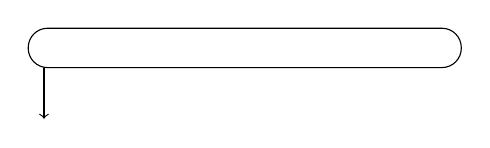
\begin{tikzpicture}\draw[rounded corners=7pt](0,0) rectangle(5.5,.5);\draw[->](.2,0)--(.2,-.65);\end{tikzpicture}}
\mspage{8}
\scanpage{10}
Groupes loc. lib. en car. $p$ (pas néc. annu par $p$)

a) Cristal de prés. finie sur $S_{\mathrm{cris}}/\deleted{\unsure{\mathbb F_p}}\mathbb Z_p$

\deleted{(\unsure{pas néc. lib.} \unsure{De dim pro}}
d'amplitude parfaite $\subset[-1,0]$, soit $\mathcal M$,
avec structures $F_{\mathcal M}$ et $V_{\mathcal M}$.

\deleted{\unsure{b)}}
On en déduit deux triangles exacts de complexes avec $F,V$ sur $S_{\mathrm{cris}}/\mathbb F_p$

$(\mathrm I)$
\diagram{\begin{tikzcd}[column sep=small]
&\mathcal M\overset L\otimes/V\arrow[dl,"\partial_{\mathrm I}"']&\\
\mathcal M\overset L\otimes/F\arrow[rr,"i_{\mathrm I}"]&&\mathcal M^{(p)}\overset L\otimes/p\simeq\varphi^*(\Delta^*)\arrow[ul,"\pi_{\mathrm I}"']
\end{tikzcd}}
\margin{$\Delta^*=\varepsilon^*(\mathbb\Delta^*)$}
\deleted{$\unsure{\mathbb\Delta^*(\mathcal M)}$}

$(\mathrm {II})$
\diagram{\begin{tikzcd}[column sep=small]
&\mathcal M\overset L\otimes/F\arrow[dl]&\\
\mathcal M\overset L\otimes/V\arrow[rr]&&\mathcal M\overset L\otimes/p=\mathbb\Delta^*\arrow[ul]\arrow[d,equal,"\mathrm{dfn}"]\\
&&L\alpha^*(\mathcal M)
\end{tikzcd}}
\margin{$\alpha:S_{\mathrm{cris}}/\mathbb F_p\longrightarrow S_{\mathrm{cris}}/\mathbb Z_p$}

b) \deleted{\unsure{Complexe}} Descente à $S_{\mathrm{zar}}$ (via $\varphi$) de la ``filtration'' $(\mathrm I)$ sur $\varphi^*(\Delta^*)$, en un triangle exact
\diagram{\begin{tikzcd}&\check\ell'_{\bullet}\arrow[dl,"\partial_0"']&\\\ell_{\bullet}[-1]\arrow[rr,"i_0"]&&\Delta^*\arrow[ul,"\pi_0"']\end{tikzcd}}
\figure{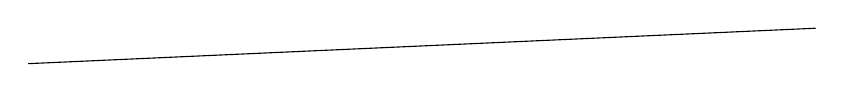
\begin{tikzpicture}\draw(0,0)--(10,.45);\end{tikzpicture}}

Prolongement à un \unsure{épaississement} p. div. $S'$ de $S$
(\unsure{c.à.d.} avec $\unsure{S}=\uline{\operatorname{Var}}(p.1_S)$) On considère
\[
\mathcal M\overset L\otimes\mathcal O_{S'}=\Delta^*(S'),
\]
qui prolonge $\Delta^*$, et il faut se donner un prolongement de la filtration b) de $\Delta^*$ en
\diagram{\begin{tikzcd}&\overline{\check\ell'_{\bullet}}\arrow[dl,"\bar\partial_0"']&\\\bar\ell_{\bullet}[-1]\arrow[rr,dash,"\bar i_0"]&&\Delta^*(S')\arrow[ul,"\pi_0"']\end{tikzcd}}
\mspage{9}
\scanpage{11}
\mspage{32}
\figure{\begin{tikzpicture}\draw[->](0,2.4)--(0,0);\end{tikzpicture}}
\deleted{
L'assertion (iii) se traite d'une façon analogue. Puisque les foncteurs $g^*(R^qf_*)$ sont effaçables pour $q>0$ dans la catégorie des faisceaux de torsion (8.1), la bijectivité de $\varphi^n$ pour $F$ implique l'effaçabilité de $(R^nf'_*)g'^*$ pour $F$. Inversement, supposons que $\varphi^{n-1}$ soit bijectif pour $(g,f,.)$ et que $(R^nf'_*)g'^*$ soit effaçable pour le faisceau $F$. Soit d'abord $F\longrightarrow G$ un effacement de $g^*(R^nf_*)$ avec $G$ de torsion et soit $C=G/F$. Alors on peut compléter le diagramme
\[
(*)
\]
\diagram{\begin{tikzcd}[column sep=small]
g^*(R^{n-1}f_*\deleted{\unsure{)}}\inserted{(}G\inserted{)})\arrow[r]\arrow[d,"\unsure{\sim|2}"']&g^*(R^{n-1}f_*\deleted{\unsure{)}}\inserted{(}C\inserted{)})\arrow[r]\arrow[d,"\unsure{\sim|2}"']&g^*(R^nf_*\deleted{\unsure{)}}\inserted{(}F\inserted{)})\arrow[r]\arrow[d,"\varphi^n"]&{}\\
\deleted{\unsure{(}}R^{n-1}f'_*\deleted{\unsure{)}}\inserted{(}g'^*G\inserted{)}\arrow[r]&\deleted{\unsure{(}}R^{n-1}f'_*\deleted{\unsure{)}}\inserted{(}g'^*C\inserted{)}\arrow[r]&\deleted{\unsure{(}}R^nf'_*\deleted{\unsure{)}}\inserted{(}g'^*F\inserted{)}\arrow[r]&{}
\end{tikzcd}}
avec un $0$ au bout de la première ligne, ce qui implique
}
\figure{\begin{tikzpicture}\draw[->](0,2.8)--(0,0);\end{tikzpicture}}
\mspage{10}
\scanpage{12}
a) Les catégories de structures a) b) introduites précédemment définissent-elles des \uline{champs} sur $S_{\mathrm{zar}}$ ?
\margin{oui si on suppose que les \deleted{\unsure{hom}}
\deleted{$\unsure{H_0(\ell),H_0(\check\ell'[1])\simeq0}$}
\inserted{$\unsure{H_1(\ell_{\bullet})\mathbin{-}H_1(\ell'_{\bullet})}$}
\deleted{\unsure{et soient localement}}
\diagram{\begin{tikzcd}0\arrow[r]&\unsure{t^*}\arrow[r,dash]&\omega\end{tikzcd}}
avec $\unsure{\omega}\text{ et }\omega^*\ t\ t^*$ loc. libres}
\figure{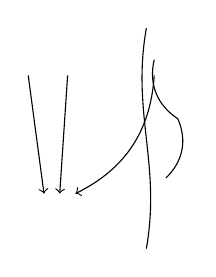
\begin{tikzpicture}\draw(0,0) to[out=80,in=260] (0,2.8);\draw[->](-1.5,2.2)--(-1.3,.7);\draw[->](-1,2.2)--(-1.1,.7);\draw[->](.1,2.2) to[bend left=30](-.9,.7);\draw(.1,2.4) to[bend right=35](.4,1.65) to[bend left=35](.25,.9);\end{tikzpicture}}

b) le foncteur ``oubli partiel'' \inserted{(de $\mathcal C$ de b))} allant vers les cristaux $\mathcal M$ sur $S_{\mathrm{cris}}/\mathbb F_p$ est-il \uline{fidèle} ?

c) Le foncteur naturel $\unsure{\mathcal M_\omega|\mathcal M\to}$ des modules loc. libres $\omega$ sur $S_{\mathrm{zar}}$, avec $F_\omega,V_\omega$, vers les structures a), b), est-il pleinement fidèle (NB il est fidèle); l'est-il du moins \deleted{\unsure{pour de}} \deleted{si $F_\omega=0$} sur la sous-catégorie définie par $F_\omega=0$; l'est il \inserted{$\operatorname{Ker}F=\operatorname{Im}V$} ?

d) Peut-on à $(\omega,F_\omega,V_\omega)$ associer un schéma en groupes fini loc libre sur $S$ ?
\mspage{11}
\scanpage{13}
Cas des groupes BT tronqués annulés par $p$.

Signifie que $F_{\mathcal M},V_{\mathcal M}$ forment suite exacte
\[
\Longleftrightarrow F_M,V_M\quad\text{\unsure{forme|forment} suite exacte}\;\ldots\ldots
\]
Alors la donnée b) implique, passant au $\underline H^1$
\margin{$\left[\begin{aligned}
\omega&=\underline H^1(\ell_\bullet[-1])\\
&=\underline H^0(\ell_\bullet)\\
\nu'&=\underline H^1(\check\ell'_\bullet)
\end{aligned}\right]$\par
$(\omega,\nu'\text{ loc. libres})$}
$M\inserted{{}=\varepsilon^*(\mathcal M)}$ filtré par
\[
0\mathbin{-}\omega\mathbin{-}M\mathbin{-}\nu'\longrightarrow0
\]
de façon que dans
\diagram{\begin{tikzcd}[column sep=small]
0\arrow[r,dash]&\varphi^*(\omega)\arrow[r]&\varphi^*(M)\arrow[r,dash]\arrow[d,equal]&\varphi^*(\nu')\arrow[r,dash]&0,\\
&&\mathcal M^{(p)}&&
\end{tikzcd}}
$\varphi^*(\omega)$ ne soit autre que $\operatorname{Im}(\mathcal M\xrightarrow{V_{\mathcal M}}\mathcal M^{(p)})$.
\margin{\uline{Cela détermine}\par\uline{$\omega$ de façon}\par\uuline{unique !}}

De $=$, passant au $\underline H^0$, on trouve
\margin{$\left[\begin{aligned}
\unsure{n|\nu}&=\underline H^0(\ell_\bullet[-1])\\
&=\underline H^{-1}(\ell_\bullet)\\
t'&=\underline H^0(\check\ell'_\bullet)
\end{aligned}\right]$}
\[
0\mathbin{-}\unsure{n|\nu}\mathbin{-}M\mathbin{-}t'\mathbin{-}0
\]
de façon que dans
\[
0\mathbin{-}\varphi^*(\unsure{n|\nu})\mathbin{-}\varphi^*(M)\mathbin{-}\varphi^*(t')\mathbin{-}0
\]
on ait
\[
\varphi^*(\unsure{n|\nu})=\operatorname{Ker}(\mathcal M^{(p)}\overset{F_{\mathcal M}}{\mathbin{-}}\mathcal M)
\]
Comme $\operatorname{Ker}F_{\mathcal M}=\operatorname{Im}V_{\mathcal M}$, on en conclut
\[
\varphi^*(\unsure{n|\nu})=\varphi^*(\omega)\qquad\text{d'où }\boxed{\unsure{n|\nu}=\omega},\quad\boxed{t'=\nu'}
\]
La seule donnée des \deleted{\unsure{suffit}}\inserted{$\mathcal M,F_{\mathcal M},V_{\mathcal M}\ (\Rightarrow\omega\unsure{\subset}M=\varphi^*(\mathcal M))$} permet elle de récupérer toute la donnée b) ? On voit qu'on pourra construire
\[
\omega\xrightarrow{V_\omega}\omega^{(p)},\qquad t'^{(p)}\xrightarrow{F_{t'}}t'
\]
\margin{$(\omega'=\check t',\quad\omega'\overset{V_{\omega'}}{\underset{\Vert\,{}^tF_{t'}}{\mathbin{-}}}\omega'^{(p)})$}
Car:
\[
\omega^{(p)}=\operatorname{Im}(M\deleted{^{\unsure{p}}}\overset{V_M}{\mathbin{-}}M^{(p)}),
\]
donc $V_M|\omega$ applique $\omega$ dans $\omega^{(p)}$
\[
t'^{(p)}=\operatorname{Coker}(M\xrightarrow{V_M}M^{(p)}),
\]
donc $F_M:M^{(p)}\to M$ se factorise par $t'^{(p)}\unsure{\mathbin{-}|\hookrightarrow}M$, d'où $F_{t'}:t'^{(p)}\to M\to t'$.
\margin{\deleted{\diagram{\begin{tikzcd}[column sep=small,row sep=small]
M\arrow[r]\arrow[d,"V_M"']\arrow[dr]&\omega\\
M^{(p)}\arrow[r,dash]&\omega^{(p)}\arrow[u,"F_\omega"']
\end{tikzcd}}}
\deleted{\diagram{\begin{tikzcd}[column sep=small,row sep=small]
M\arrow[r]\arrow[d]&t\\
M^{(p)}\arrow[r]&\unsure{t^{(p)}}
\end{tikzcd}}}}
\mspage{12}
\scanpage{14}
\diagram{\begin{tikzcd}[column sep=large,row sep=large]
M\arrow[r]\arrow[d,"V_M"']\arrow[dr,two heads,"\text{épi}"]&\omega\arrow[d,"V_\omega"]\\
M^p\arrow[r]&\omega^{(p)}
\end{tikzcd}}
\diagram{\begin{tikzcd}[column sep=large,row sep=large]
\unsure{M^p|M}\arrow[r,two heads]&t'\\
M^{(p)}\arrow[u]\arrow[r]&t'^{(p)}\arrow[u,"F_t"]\arrow[ul,hook]
\end{tikzcd}}

\deleted{On peut \unsure{donc} former} On aura
\diagram{\begin{tikzcd}[column sep=small,row sep=large]
&&\unsure{0}\arrow[d]&&\\
&\deleted{\unsure{\omega}\mathbin{-}\unsure{\omega}}&\unsure{t'^p}\arrow[d]\arrow[dr,"F_{t'}"]&&\\
0\arrow[r,dash]&\omega\arrow[r,dash]\arrow[dr,"V_\omega"']&M\arrow[r,dash]\arrow[d]&t'\arrow[r,dash]&0\\
&&\omega^p\arrow[d]&&\\
&&0&&
\end{tikzcd}}
\mspage{13}
\scanpage{15}
\mspage{33}
l'injectivité de $\varphi^n$. Soit maintenant $F\longrightarrow G$ un effacement de $(R^nf'_*)g'^*$ avec $G$ de torsion, et soit $C=G/F$. Alors on peut compléter le diagramme $(*)$ par un $0$ au bout de la deuxième ligne, ce qui implique la surjectivité de $\varphi^n$. La dernière assertion de (iii) est immédiate à partir de la première.

\uline{Lemme(8.3):} Soit
\diagram{\begin{tikzcd}[column sep=small]
\deleted{\unsure{X}}&X\arrow[dr,"f"']&&\bar X\arrow[ll,"\pi"']\arrow[dl,"\bar f"]\\
&&S&
\end{tikzcd}}
un diagramme commutatif de morphismes propres. Supposons\deleted{\unsure{e}} que $\pi$ soit surjectif. Notons par un \deleted{sigle le}\inserted{``prime'' l'effet d'un} changement de base $g:S'\longrightarrow S$, et soient $g':X'\longrightarrow X$ et $\bar g:\bar X'\longrightarrow\bar X$ les morphismes \deleted{déduits}\inserted{canoniques}.

(i) \deleted{Si (5.1)(i) est vrai pour $(g,\bar f,.)$ et pour $(g',\pi,.)$ il l'est pour $(g,f,.)$.} \inserted{Assertion vide.}

(ii) Supposons que (5.1)(i) soit vrai pour $(g,f,.)$, $(g,\bar f,.)$ et $(g',\pi,.)$. Si (5.1(ii)) est vrai pour $(g,\bar f,.)$ \deleted{\unsure{et pour} $\unsure{(g',\pi,.)}$} il l'est pour $(g,f,.)$.

(iii) Si (5.1)(iii) est vrai pour $(g,\bar f,.)$ et pour $(g',\pi,.)$, il l'est pour $(g,f,.)$.

\deleted{Démonstration. (i): Supposons d'abord que le faisceau $F$ sur $X$ est de la forme $F=\pi_*G$. On a}
\mspage{14}
\scanpage{16}
\[\mathbf M\]
\[
X_{\mathrm{cris}\,0}\hookrightarrow X_{\mathrm{cris}/\unsure{n}}
\qquad 0\mathbin{-}G\hookrightarrow G'\longrightarrow G''\longrightarrow0
\]
\[\mathcal M''\longrightarrow\unsure{\mathcal M'|\mathcal M^\bullet}\]
\figure{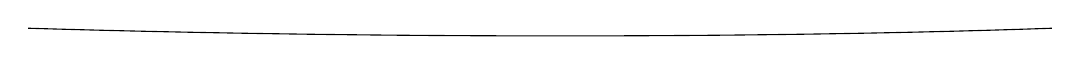
\begin{tikzpicture}\draw (0,0) .. controls (4,-.12) and (9,-.14) .. (13,0);\end{tikzpicture}}

$1^\circ)$ Cristal de \unsure{prés. finie} $\mathcal M$ sur $S_{\mathrm{cris}}/\mathbf F_p$

\deleted{\unsure{$2^\circ$}} avec $F_{\mathcal M},V_{\mathcal M}$,

d'où
\diagram{\begin{tikzcd}[column sep=small]
&L'(\mathcal M)\arrow[dl]&&\\
L_\bullet(\mathcal M)\arrow[rr,dash]&&\Delta^*(\mathcal M^{\unsure{p|(p)}})\arrow[ul]&\mathrm I(\mathcal M)
\end{tikzcd}}
\diagram{\begin{tikzcd}[column sep=small]
&L_\bullet(\mathcal M)\arrow[dl]&&\\
L'(\mathcal M)\arrow[rr,dash]&&\Delta^*(\mathcal M)\arrow[ul]&\mathrm{II}(\mathcal M)
\end{tikzcd}}
Soit $\varepsilon^*(\mathcal M)=M$

$2^\circ)$ Triangle
\diagram{\begin{tikzcd}[column sep=small]
&&\unsure{\mathcal T_2|\tau_2}\arrow[dl]&&\\
\unsure{\mathcal T|\tau}:&\unsure{\mathcal T_0|\tau_0}\arrow[rr,dash]&&\unsure{\mathcal T_1|\tau_1}\arrow[ul]&
\end{tikzcd}}
\margin{(ou $F$-$V$-triangle ?)}
sur $S_{\mathrm{Zar}}$ de complexes parfaits d'ampl. \unsure{p-faite|p-finie} $\subset[-1,0]$

$3^\circ)$ Isom de (vrais) triangles (ou $F$-$V$-triangles ?)
\[\varphi^*(\unsure{\mathcal T|\tau})\overset\alpha\simeq\mathrm I(\mathcal M)\]

$4^\circ)$ Isom (ou $F$-$V$-isom ?)
\[\unsure{\mathcal T_1|\tau_1}\overset\beta\simeq\varepsilon^*(\Delta^*(\mathcal M))\deleted{\unsure{\simeq}}\]
tel qu'on ait commutativité
\diagram{\begin{tikzcd}[column sep=large,row sep=large]
\varphi^*(\unsure{\mathcal T_1|\tau_1})\arrow[r,"\alpha_1"]\arrow[dr,"\varphi^*(\beta)"']&\unsure{\mathbb\Delta^*|\Delta^*}(\mathcal M)^{(p)}\\
&\varphi^*\varepsilon^*(\Delta^*(\mathcal M))\simeq\Delta^*(\mathcal M)^{(p)}\arrow[u,Rightarrow,"\mathrm{id}"']
\end{tikzcd}}
\mspage{15}
\scanpage{17}
\deleted{
\textcircled{3} Indétermination dans ces données, pour $(\deleted{\unsure{G}}\mathcal M,T)$ (i.e. $G$) fixé.

La catégorie des données \deleted{\unsure{$t$}} en question est \deleted{\unsure{équiv.}} ``un torseur'' pour la catégorie des torseurs sous $\mu_2$ sur $A$, donc l'ensemble des classes d'isomorphie de ces structures est \inserted{un torseur sous}
\[
H^1(A\deleted{^{\unsure{*}}},\mu_2)\simeq\prod_p\mathbf Q_p^*/\mathbf Q_p^{*2},
\]
\margin{\unsure{modulo} une légère \unsure{restriction} en $2$, \unsure{donnée} à l'$\infty$}
\margin{\unsure{pr. direct local rel. à l'un des sous-grps}\par$\mathbf Z_p^*/\mathbf Z_p^{*2}$}
l'ensemble des autom. d'un objet de la catégorie est
\[H^0(A',\mu_2)=\prod_p(\mathbf Z/2\mathbf Z)\]

\textcircled{4} Rigidité de $\mathcal M$ pour les structures \unsure{enrichies}.

Soit $(\mathcal M',T')$ muni des $=$ données \inserted{suppl.} que $(\mathcal M,T)$. On se demande de déterminer la catégorie des équivalences
\[
(\mathcal M,T,\overbrace{\bar T_{A'},u_{A'}}^{t_{A'}},t_\infty,t_p)\longrightarrow(\mathcal M',T'\text{ etc\quad})
\]
\inserted{Cette catégorie est vide, \uline{ou}} \deleted{Elle} forme un torseur pour la catégorie des torseurs sous $\mu_2$ sur $\mathbf Q$, \uline{munis} d'une trivialisation \deleted{\unsure{de celle}} au dessus \deleted{de} $A$. Cette dernière catégorie a comme \deleted{\unsure{ensemble}} \deleted{de} classes d'objets à isom près le groupe
\[
H^1(\mathbf Q\mathbin{\mathrm{mod}}A,\mu_2)\simeq {}_2(\unsure{\mathcal J_{\mathbf Q}|\mathfrak I_{\mathbf Q}})\simeq(\prod_p\mathbf Z/2\mathbf Z)/(\pm1)
\]
\margin{qui a la\par puiss. du\par continu $\big]$}
d'autre part cette catégorie est rigide $(H^0(\mathbf Q\mathbin{\mathrm{mod}}A,\mu_2)=0)$.

Comme l'image de $H^1(\mathbf Q\mathbin{\mathrm{mod}}A,\mu_2)$ dans $H^1(\mathbf Q,\mu_2)$ est nulle, on voit que \uline{l'équivalence restreinte entre} $(\mathcal M,T)$ \uline{et} $(\mathcal M',T')$ \uline{est déterminée à isom unique près}. Donc on peut identifier sans dommages $(\mathcal M,T)$ et $(\mathcal M',T')$
}
\mspage{16}
\scanpage{18}
Soit $\omega$ sur $S_{\mathrm{Zar}}$, avec $F_\omega,V_\omega$, on lui associe

$1^\circ)$ $\mathcal M=\varphi^*(\omega),\quad F_{\mathcal M}=\varphi^*(F_\omega),\quad V_{\mathcal M}=\varphi^*(V_\omega)$
\margin{$M=\omega^p$\par
$\varepsilon^*(\Delta(\mathcal M))=\Delta^*(\omega)$\par
\unsure{complexe can. ext.}\par de $\omega^p$ par $\omega^p$}

$2^\circ)$ Triangle
\diagram{\begin{tikzcd}[column sep=small,row sep=large]
&&\mathcal T_2^{(\omega)}=[\omega\overset{V_\omega}{\mathbin{-}}\omega^p]\arrow[dl,"1"']&\\
\unsure{\mathcal T(\omega)|\mathbb T(\omega)}\unsure{:=|:}&\mathcal T_0^{(\omega)}=[\omega^p\xrightarrow{F_\omega}\omega]\arrow[rr]&&\mathcal T_1^{(\omega)}=[\omega^{(p)}\overset0{\mathbin{-}}\omega^{(p)}]\arrow[ul]
\end{tikzcd}}
\unsure{déduit} de $\omega$\quad $(\mathcal T_1^{(\omega)}=\Delta^*(\omega))$

$3^\circ)$ Isom \uuline{can}
\[\varphi^*(\mathcal T(\omega))\overset{\alpha_\omega}\simeq\mathcal T(\varphi^*(\omega))\]

$4^\circ)$ L'\uline{identité}
\[\mathcal T(\omega)_1\overset{\beta_\omega}\simeq\varepsilon^*(\Delta^*(\mathcal M))\simeq[\omega^p\overset0{\mathbin{-}}\omega^p]\]

\uline{Question} Le foncteur
\[
(\omega,F_\omega,V_\omega)\longmapsto(\varphi^*(\omega),\varphi^*(F_\omega),\varphi^*(V_\omega),\mathcal T(\omega),\alpha_\omega,\beta_\omega)
\]
est-il pl. fidèle ?? L'est-il du moins sur la sous-catégorie des triples $(\omega,F_\omega,V_\omega)$ avec $F_\omega=0$ ?
\figure{\begin{tikzpicture}\draw (0,0)--(14,.8);\end{tikzpicture}}

\[
\left\{\begin{aligned}
\varphi^*(\omega)&\xrightarrow{u}\varphi^*(\omega')\\
\mathcal T(\omega)&\overset{\unsure{v|\sigma}}{\mathbin{-}}\mathcal T(\omega')
\end{aligned}\right.
\]
\margin{$u$ compatible avec $F,V$\par
$\unsure{v|\sigma}$ hom de vrais triangles\par
$v_1$ déterminé comme $\varepsilon^*(u)$}
commutativité du diagramme
\diagram{\begin{tikzcd}[column sep=large,row sep=large]
\mathcal T_1(\omega)\arrow[r,"v_1"]\arrow[d,Rightarrow,"\beta_\omega"']&\mathcal T_1(\omega')\arrow[d,Rightarrow,"\beta_{\omega'}"]\\
\varepsilon^*(\Delta^*(\varphi^*(\omega)))\arrow[d,equal]&\varepsilon^*(\Delta^*(\varphi^*(\omega')))\arrow[d,equal]\\
\Delta^*(\omega)\arrow[r,"\varepsilon^*(u)"']&\Delta^*(\omega')
\end{tikzcd}}
\margin{$\varphi^*(\unsure{v|\sigma})$ déterminé par $u$ comme $\mathcal T(u)$}
\diagram{\begin{tikzcd}[column sep=large,row sep=large]
\varphi^*(\mathcal T(\omega))\arrow[r,dash,"\alpha_\omega","\sim"']\arrow[d,"\unsure{\varphi^*(\omega)|\varphi^*(v)}"']&\mathcal T(\varphi^*(\omega))\arrow[d,"\mathcal T(u)"]\\
\varphi^*(\mathcal T(\omega'))\arrow[r,dash,"\alpha_{\omega'}","\sim"']&\mathcal T(\varphi^*(\omega'))
\end{tikzcd}}
\mspage{17}
\scanpage{19}
\begin{flushright}Tribu n° 66\end{flushright}
\begin{center}
\uline{DÉCISIONS sur l' INTÉGRATION}

(Rédactions n° 446 et 447)

\unsure{-:-:-:-}
\end{center}

\uline{La réédition d'Intégration V} (n° 446).

Le projet de réédition est adopté d'enthousiasme. Comme la Tribu a dormi ou a mis la chaudière en marche pendant certaines discussions, que Meyer et Douady ont noté les décisions d'ordre rédactionnel, et qu'ils ont commencé à les mettre à exécution, on ne trouvera pas grand chose dans ce qui suit. Meyer et Douady sont en train de faire la rédaction définitive, dont de rares exemplaires circuleront. A l'impression ensuite !

On remplace la notation $\unsure{\widetilde\mu^*}$ par $\mu^0$. On dira `` modérée '' au lieu de `` tempérée'' (déf. 2, p. 4) ; vive Pinay ! On donnera un sorite des fonctions, ensembles et mesures modérées. Les pages 12 à 19 de la rédaction 446 sont supersédées par la suite.

On dira `` scalairement essentiellement intégrable '' (resp. `` scalairement intégrable '') pour la notion du bas de la p. 20. Dans la déf. 1, p. 21, on dira `` $\mu$-adéquate '' (ça généralise la notion de l'édition actuelle ; la déf. 2 est ainsi remplacée par une remarque, qui le dira).

Certains ont été effrayés par le nombre de chapeaux emboîtés, et proposent qu'on fasse des dépliants indiquant les chapeaux et leurs domaines de validité. L'idée a été repoussée.

\uline{Les mesures sur les espaces séparés} (n° 447).

A la lecture de cette rédaction Bourbaki a versé des larmes grosses comme des bouchons de carafe, regrettant de n'avoir pas limité les chap. III et IV aux mesures sur les compacts et de n'être pas ensuite passé directement aux espaces séparés généraux. Bref, c'est la ressurection triomphante des compactologies. Mais il est trop tard pour bouleverser encore les chap. III et IV. Hélas, hélas, hélas !

Comme le contenu du n° 447 n'a pas beaucoup plus à voir avec le chap. V qu'avec les autres, il formera un chapitre séparé, qui viendra à la fin du Livre (Chap. IX) ; un ``Leitfaden'' dira de quoi il dépend.

Douady et Meyer feront la rédaction suivante, qui sera tirée et éventuellement relue en Congrès. Schwartz fournira un papier sur la mesure de Wiener-\unsure{Levy|Lovy} sur $\mathcal C([0,1])$.
\mspage{18}
\scanpage{20}
\diagram{\begin{tikzcd}[column sep=small]
&L'\arrow[dl]&\\
L.\arrow[rr]&&\underbrace{\Delta(\mathcal M)}_{H_1^{\unsure{\bullet}}\quad H_0}\arrow[ul]
\end{tikzcd}}
\diagram{\begin{tikzcd}[column sep=small]
&\mathcal M_{/V}\deleted{\unsure{F}}\arrow[dl]&\\
\mathcal M_{/F}\arrow[rr]&&\mathcal M_{/p}^{\unsure{(p)}}=\varphi^*(\Delta(\mathcal M))\arrow[ul]
\end{tikzcd}}
\diagram{\begin{tikzcd}[column sep=small]
&&&&&\Theta\arrow[dr]&\\
0\arrow[r,dash]&{}_F\mathcal M^{\unsure{\sigma}}\arrow[r,dash]&{}_p\mathcal M^{\unsure{\sigma}}\arrow[r,dash,"F"]&{}_V\mathcal M\arrow[rr,dash]\arrow[urr]&&\mathcal M_p\arrow[r,"V"]&\mathcal M_p^{\unsure{\sigma}}\arrow[r,dash]&\mathcal M_V^{\unsure{\sigma}}\arrow[r]&0
\end{tikzcd}}
\[0\longrightarrow\unsure{n|u}\longrightarrow\mathbb D_1\mathbin{-}t^*\mathbin{-}\omega\longrightarrow\mathbb D_0\longrightarrow\nu^*\longrightarrow0\]
\diagram{\begin{tikzcd}X_{\mathrm{cris}}\arrow[d,"\varphi"]\\X_{\mathrm{Zar}}\end{tikzcd}}
\diagram{\begin{tikzcd}[column sep=small,row sep=small]
J\arrow[r,hook]\arrow[d]&B\arrow[r]\arrow[d,"\unsure{\mu}"']&A\arrow[d]\arrow[dr,"\lambda\mapsto\lambda^p"]\arrow[dddr,dash,"\deleted{\unsure{\longrightarrow}}"']&\\
\unsure{\gamma^p}\;JB'\arrow[r,hook]\arrow[d,equal]&B'\arrow[r]\arrow[d,equal]&B'/JB'\arrow[r]\arrow[d,equal]&A\\
J^{\unsure{(p)}}&\mathbf B&B/J^{(p)}B\arrow[d]\arrow[dr]&\\
&\deleted{\unsure{B}}&\deleted{\unsure{C}}\arrow[r]&C\arrow[uu]\\
&&B\arrow[ur]\arrow[uu,bend left,dashed]&B\mathbin{-}A\\
&&&B\unsure{\otimes}B\longrightarrow A
\end{tikzcd}}

\deleted{$a)$ descendre $\mathcal M_{/F}$ et $\mathcal M_{/V}$}

\deleted{$b)$ descendre le triangle tout entier}

\diagram{\begin{tikzcd}[column sep=small,row sep=small]
J^{(p)}B\arrow[dr]&J\arrow[r,hook]\arrow[dr]&B\arrow[r,dash]\arrow[dr]&A\arrow[dr,equal]&\\
&0&\underset{\text{r.d.}}{I}\arrow[r,hook]&C\arrow[r]&A
\end{tikzcd}}
\[\underbrace{\widetilde\Delta(\mathcal M)}_{\deleted{\unsure{D}}\;\widetilde D_1\quad\widetilde D_0}\]
\[
0\longrightarrow\deleted{\unsure{n}}\longrightarrow D_1\mathbin{-}\widetilde D_1\longrightarrow0
\qquad
0\longrightarrow\widetilde D_0\mathbin{-}D_0\mathbin{-}\nu^*\longrightarrow0
\]
\margin{[\unsure{uniquement déterminés} par $I(\mathcal M)$]}

$(i)$
\diagram{\begin{tikzcd}[column sep=small]
&&&\unsure{\vartheta}\arrow[dr]&&\\
0\arrow[r,dash]&\widetilde D_{\unsure{1}}\deleted{\unsure{\prime}}\arrow[r,dash]&t^*\arrow[r]\arrow[ur]&\omega\arrow[r]&\widetilde D_0\arrow[r]&0
\end{tikzcd}}
\margin{On descend $\Theta$ en $\unsure{\vartheta}$,\par
et \deleted{\unsure{obtenons directement}} \unsure{non de la $\Theta$}\par
en extension de $\unsure{D'_0}$ par $\unsure{\vartheta}$\par
\deleted{\unsure{à coefficients}} de $\unsure{\vartheta}$ par $D'_1$\par
\deleted{\unsure{A}}}

\figure{\begin{tikzpicture}\draw (0,0)--(.7,0);\end{tikzpicture}}

$(ii)$
\diagram{\begin{tikzcd}[column sep=small]
&t^*[1]\arrow[dl,"1"']&\deleted{\unsure{\vartheta}}\\
\omega\arrow[rr]&&\widetilde\Delta(\mathcal M)\arrow[ul]
\end{tikzcd}}
\margin{\unsure{connu}}
\deleted{\unsure{à expliciter}} descend
\diagram{\begin{tikzcd}[column sep=small]
&{}_V\mathcal M[1]\arrow[dl]&\\
\mathcal M_F\arrow[rr,dash]&&\varphi^*(\widetilde\Delta(\mathcal M))\arrow[ul]\arrow[d,equal]\\
&& (\mathcal M_{/p})'
\end{tikzcd}}

\diagram{\begin{tikzcd}[column sep=small,row sep=small]
&\widetilde X\arrow[r,shift left]\arrow[r,leftarrow,shift right]\arrow[d,dash]&\widetilde{X\times X}\arrow[r,equal]&\unsure{\widetilde{X\times X\times X}}\\
\unsure{S}\arrow[r,hookleftarrow,"\unsure{c}"]&X\arrow[r,equal]\arrow[d,dash]&X\times X\arrow[r,equal]&\unsure{X\times X\times X}\\
S'\arrow[r,equal]\arrow[d]\arrow[ddd,bend right=55,"F_S"']&S\arrow[r,equal]\arrow[d]&S\arrow[d]&\\
\widetilde{\deleted{\unsure{X}}X}\arrow[d]&\widetilde{X\times X}\arrow[l,shift left]\arrow[l,shift right]\arrow[d]&\widetilde{X\times X\times X}\arrow[l,shift left=1.5ex]\arrow[l]\arrow[l,shift right=1.5ex]\arrow[d]&\\
\widetilde X\arrow[u,bend left,dashed]\arrow[d,"\text{plat}"']&\widetilde{X\times X}\arrow[l,shift left]\arrow[l,shift right]\arrow[u,bend left,dashed]\arrow[d,"\text{plat}"]&\widetilde{X\times X\times X}\arrow[l,shift left=1.5ex]\arrow[l]\arrow[l,shift right=1.5ex]\arrow[u,bend left,dashed]\arrow[d,"\text{plat}"]&\\
S\arrow[r,equal]&S\arrow[r,equal]&S&
\end{tikzcd}}

i.e. on doit \deleted{\unsure{donner}} \inserted{\unsure{améliorer|considérer}} les isom.
\[
[t^*\deleted{\unsure{[1]}}\longrightarrow\omega]\deleted{\unsure{[1]}}\simeq\widetilde\Delta(\mathcal M)
\]
\unsure{descendant l'isom.} \illegible{2} \unsure{par un} $\varphi^*$ \unsure{de} $\Delta'(\mathcal M)$.

l'arbitraire est dans \unsure{extensions identiquement} $0$ sur \unsure{cris après} $\varphi^*$

i.e. dans $\operatorname{Ext}^1(\widetilde D_0,\widetilde D_1)$ ou plus précisément, sans doute, dans
\[
\operatorname{Ext}^1(S_{\mathrm{Zar}}\ \mathrm{mod}\ S_{\mathrm{cris}};\widetilde D_0,\widetilde D_1);
\]
les \unsure{autos} de la \unsure{situation sont}
\[
\text{dans}\qquad\operatorname{Ext}^0(S_{\mathrm{Zar}}\ \mathrm{mod}\ S_{\mathrm{cris}};\widetilde D_0,\widetilde D_1)=0\quad!
\]
\margin{\unsure{Obstruction au théorème}}
\[
\text{dans}\qquad\operatorname{Ext}^2(S_{\mathrm{Zar}}\ \mathrm{mod}\ S_{\mathrm{cris}};\widetilde D_0,\widetilde D_1).
\]
\mspage{19}
\scanpage{21}
\begin{center}- 65 -\end{center}
PROPOSITION 2 (lemme de Schwarz).-- \uline{Soit} $f$ \uline{une fonction holomorphe dans un domaine} $A\subset\mathbb C$ \uline{contenant le disque} $|z|\leq1$, \uline{et supposons que} $f$ \uline{ait un zéro d'ordre k au point} $z=0$. \uline{Dans ces conditions, si M est le maximum de} $\|f(z)\|$ \uline{pour} $|z|=1$, \uline{on a} $\|f(z)\|\leq M|z|^k$ \uline{pour tout} $z$ \uline{tel que} $|z|\leq1$.

Il suffit de remarquer que $z^{-k}f(z)$ est holomorphe dans $A$ et que le maximum de $\|z^{-k}f(z)\|$ pour $|z|=1$ est égal à $M$.

\uline{6. Ensembles équicontinus de fonctions holomorphes.}

PROPOSITION 3.- \uline{Soit} $A\subset\mathbb C^p$ \uline{un domaine}, $\Phi$ \uline{un ensemble de fonctions holomorphes dans} $A$, \uline{à valeurs dans un espace de Banach E}. \uline{Si les fonctions de} $\Phi$ \uline{sont uniformément bornées dans toute partie compacte de} $A$, $\Phi$ \uline{est un ensemble équicontinu dans} $A$.

En effet, soit $a$ un point de $A$, $P$ un polycylindre fermé de centre $a$ et de rayons $\rho$, contenu dans $\unsure{P|A}$. Par hypothèse, il existe un nombre $M$ tel que $\|f(z)\|\leq M$ pour tout $z\in P$. Soit $Q$ le polycylindre fermé de centre $a$ et de rayons $\rho/2$ ; pour tout $x\in Q$, le polycylindre fermé de centre $x$ et de rayons $\rho/2$ est contenu dans $P$, donc la formule (5) du § 3 donne en particulier les majorations
\[
(3)\qquad\|\partial f/\partial z_k\|\leq2M/\rho
\]
valables pour tout $x\in Q$ et toute fonction $f\in\Phi$. Or, on peut écrire, pour tout $y\in Q$
\[
f(y)-f(a)=\int_\sigma\left(\sum_k\frac{\partial f}{\partial\unsure{x_k|z_k}}\,dz_k\right)
\]
l'intégrale étant prise le long du segment $\sigma:t\longrightarrow a+t(y-a)$, avec $0\leq t\leq1$ ; on en déduit immédiatement, compte-tenu de (3), que
\[
\|f(y)-f(a)\|\leq\frac{2pM}{\rho}|y-a|
\]
pour \uline{toute} fonction $f\in\Phi$ et tout $y\in Q$, d'où la proposition.
\mspage{20}
\scanpage{22}
\deleted{\unsure{2}}
\diagram{\begin{tikzcd}[column sep=small]
&\check\ell'[1]\arrow[dl]&\\
\ell\arrow[rr]&&\Delta\arrow[ul]
\end{tikzcd}}
\[
0\longrightarrow\ell\mathbin{-}\Delta\mathbin{-}\check\ell'[1]\mathbin{-}0
\]
\[
0\longrightarrow0\mathbin{-}\Theta\overset\sim\longrightarrow\Theta\longrightarrow0
\]
\[
\begin{array}{ll}
\mathrm{Fil}^0\Theta=\Theta&\mathrm{Fil}^0(\Delta)=\Delta\\
\mathrm{Fil}^1\Theta=0&\mathrm{Fil}^1(\Delta)=\ell\\
&\mathrm{Fil}^2(\Delta)=0
\end{array}
\]
\diagram{$\left.\begin{array}{rcl}\Delta&\longrightarrow&\Theta\\\ell&\longrightarrow&0\end{array}\right]\quad\text{i.e.}\quad\check\ell'[1]\longrightarrow\Theta$}
\margin{modulo les diff. d'\unsure{hom}\par \unsure{de complexes filtrés}}

\diagram{\begin{tikzcd}[column sep=large,row sep=large]
\operatorname{Hom}_{\mathrm D(X)}(\check\ell'[1],\Theta)\arrow[r]\arrow[d]&\operatorname{Hom}(\Delta,\Theta)\\
\operatorname{Hom}_{\mathrm D(X_{\mathrm{cris}})}(\varphi^*(\check\ell'[1]),\varphi^*(\Theta))&
\end{tikzcd}}
\[\Theta=\underline O_X[1]\]
\deleted{$\operatorname{Hom}_{\unsure{\mathrm D(X)}}$}
\diagram{\begin{tikzcd}[column sep=large,row sep=large]
H^0(\ell'_\bullet)\arrow[r]\arrow[d]&\mathbb H^0(\check\Delta^{\unsure{*}}\deleted{\unsure{[1]}})\\
H^0(\varphi^*(\ell'_\bullet))&
\end{tikzcd}}
\deleted{$0\mathbin{-}H^{-1}(\ell')$}
\[
0\mathbin{-}\ell'\longrightarrow\check\Delta^{\unsure{*}}\mathbin{-}\check\ell[1]\mathbin{-}0
\]
\diagram{\begin{tikzcd}[column sep=small,execute at end picture={
\draw ([xshift=-2pt,yshift=-3pt]\tikzcdmatrixname-1-2.south west) -- ([xshift=-2pt,yshift=-7pt]\tikzcdmatrixname-1-2.south west) -- ([xshift=2pt,yshift=-7pt]\tikzcdmatrixname-1-5.south east) -- ([xshift=2pt,yshift=-3pt]\tikzcdmatrixname-1-5.south east);
}]
0\arrow[r,dash]&\unsure{n}_{G^*}\arrow[r]&D^*(G)^\vee\arrow[r]&t_G\arrow[r]&\omega_{G^*}\arrow[r]&D^*(G^*)\arrow[r]&\nu_G\arrow[r]&0
\end{tikzcd}}
\[
0\mathbin{-}H^{-1}(\ell')\mathbin{-}\mathbb H^{-1}(\check\Delta^{\unsure{*}})\mathbin{-}H^{-1}(\check\ell[1])\mathbin{-}H^0(\ell')\mathbin{-}\mathbb H^0(\check\Delta^{\unsure{*}})\mathbin{-}H^0(\check\ell[1])\mathbin{-}0
\]
\[
\hspace{5em}0\mathbin{-}L'_1\longrightarrow L'_0\longrightarrow0
\]
\[
\Gamma(D^*(G)^\vee)\mathbin{-}\underbrace{\Gamma(t_G)}\longrightarrow H^0(\ell')
\]
\[
H^1(n_{G^*})\longrightarrow H^1_{\mathrm{cris}}(n_{G^*})
\]
\[
0\longrightarrow\underbrace{n_{G^*}\mathbin{-}D^*(G)^\vee}\mathbin{-}Q\longrightarrow0
\]
\[
\mathbin{-}\omega\longrightarrow D^*(G)
\]
\[
\left\{\begin{aligned}
H^1(D^*(G)^\vee)&=0\\
\operatorname{Ker}\bigl(H^1(n_{G^*})\longrightarrow H^1_{\mathrm{cris}}(n_{G^*})\bigr)&\ne0
\end{aligned}\right.
\]
\mspage{21}
\scanpage{23}
\mspage{22}
\begin{center}- 53 -\end{center}
holomorphe dans $P$ (comme fonction réciproque de $e^z$), on a $\int_\gamma\frac{dz}{z}=\log(\gamma(b))-\log(\gamma(a))$, et par suite $\unsure{\Im}(\int_\gamma\frac{dz}{z})=\mathrm{Am}(\gamma(b))-\mathrm{Am}(\gamma(a))$, en désignant par $\mathrm{Am}(z)$ la mesure de l'amplitude de $z$ appartenant à l'intervalle $\left]-\pi,+\pi\right[$. Par abus de langage, on dit encore que $\unsure{\Im}(\int_\gamma\frac{dz}{z})$ pour une route \uline{quelconque} $\gamma$ contenue dans $\unsure{\complement\{0\}|\mathbb C\setminus\{0\}}$, est la \uline{variation de l'amplitude de} $z$ \uline{le long de} $\gamma$. Si $\gamma$ est un circuit d'indice $n$ par rapport à $0$, la ``variation de l'amplitude de $z$ '' le long de $\gamma$ est donc $2n\pi$.

Les notions précédentes relatives aux chemins \uline{carrossables} peuvent s'étendre aux chemins \uline{quelconques}. Soit $\gamma$ un chemin achevé quelconque défini dans un intervalle $I=[\alpha,\beta]$ à valeurs dans $\mathbb C$, et soit $a$ un point de $\mathbb C$ n'appartenant pas à $\gamma(I)$. Il existe une déformation de $\gamma$ en un chemin carrossable $\gamma'$ \uline{dans} $\complement\{a\}$ (§ 2, prop.1) conservant les extrémités de $\gamma$ ; en outre, si $\gamma'$ et $\gamma''$ sont deux chemins carrossables déformés de $\gamma$ dans $\complement\{a\}$ par de telles déformations, $\gamma'$ et $\gamma''$ peuvent être déformés l'un en l'autre dans $\complement\{a\}$ par une déformation de même type ; en raison du cor. du th.1 du § 2, la ``variation de l'amplitude'' de $z-a$ le long de $\gamma'$ et le long de $\gamma''$ sont égales. Cette variation ne dépend donc que du chemin $\gamma$ initial, et on l'appelle encore la \uline{variation de l'amplitude de} $z-a$ \uline{le long de} $\gamma$.

Il résulte aussitôt de ces définitions que les variations de l'amplitude de $z-a$ le long de $\gamma$ et le long de l'opposé de $\gamma$ sont \uline{opposées} ; si $\gamma_1$ et $\gamma_2$ sont deux chemins dans $\complement\{a\}$ tels que la juxtaposition de ces chemins soit définie, la variation de l'amplitude de $z-a$ le long de $\unsure{\gamma_1\vee\gamma_2|\gamma_1\wedge\gamma_2}$ est la \uline{somme} des variations de l'amplitude de $z-a$ le long de $\gamma_1$ et le long de $\gamma_2$.
\scanpage{25}
\uline{Groupes de Barsotti-Tate ordinaires.}

$S_0$ schém. lisse sur $k$, corps parfait, $S_0=\operatorname{Spec}A_0$ \unsure{si on veut}

$S$ schém. formel lisse sur $W$ relevant $S_0$

$F_S$, endom \deleted{\unsure{sur la base}} du schém. formel $S$, compatible avec $\sigma$ sur $W$ (autom de Frobenius) et prolongeant $F_{S_0}$ (endom de Frob. absolu)

$\mathrm{BTO}(S_0)$ catégorie des gpes de BT ordinaires sur $S_0$

$C=\mathcal C_{S,F_S}$ catégorie des \deleted{\unsure{quintuplets}} \inserted{\unsure{n-uplets}} $(P',Q',M,\nabla,F_M,\mathrm{Fil}_0)$, formés de

$P',Q'$ faisceaux $p$-adiques constants tordus \deleted{\unsure{loc.}} loc. libres de t.f. sur $S$

$M$ extension de $P'\otimes_{\mathbb Z_p}\mathcal O_S$ par $Q'\otimes_{\mathbb Z_p}\mathcal O_S$
\[
0\mathbin{-}Q'\otimes_{\mathbb Z_p}\mathcal O_S\longrightarrow M\mathbin{-}P'\otimes_{\mathbb Z_p}\mathcal O_S\mathbin{-}0
\]
$\nabla$ connexion à courbure nulle sur $M$, \deleted{induisant sur} \inserted{compatible avec} la structure d'extension ($Q'\otimes\mathcal O_S$ et $P'\otimes\mathcal O_S$ munis de leurs connexions canoniques $\ldots$)

$F_M:F_S^*(M)\mathbin{-}M$ homomorphisme d'extensions, compatible avec les connexions induisant \deleted{sur $Q'$} respectivement
\[
F_{Q'}:F_S^*(Q'\otimes_{\mathbb Z_p}\mathcal O_S)\mathbin{-}Q'\otimes_{\mathbb Z_p}\mathcal O_S
\]
\[
p.F_{P'}:F_S^*(P'\otimes_{\mathbb Z_p}\mathcal O_S)\mathbin{-}P'\otimes_{\mathbb Z_p}\mathcal O_S,
\]
$F_{P'}$ ($F_{Q'}$) étant l'isom canonique

$\mathrm{Fil}$ un \deleted{\unsure{filtration à deux crans} de $M_0=M\otimes\mathcal O_{S_0}$} \inserted{splittage (\unsure{pas néc.} comp. aux connexions,)} de l'extension $M_0$ de $P'_0\otimes_{\mathbb F_p}\mathcal O_{S_0}$ par $Q'_0\otimes_{\mathbb F_p}\mathcal O_{S_0}$, compatible à l'hom $F_{M_0}$.

On a un foncteur canonique (``module de Dieudonné'')
\[
\mathbb D:\mathrm{BTO}(S_0)^\circ\longrightarrow C.
\]
\uline{Question}: \uline{Est-ce une équivalence de catégories ?}
\mspage{24}
\scanpage{26}
$1)$ Description de la catégorie $C$.

Considérons un objet $(P',Q',M,\nabla,F_M,\mathrm{Fil})$ \deleted{[\unsure{en oubliant pour le moment} $\nabla$]} Choisissons un splittage de l'extension $M$, d'où un isom
\[
\varphi:M\overset\sim\longrightarrow P'\otimes_{\mathbb Z_p}\mathcal O_S+Q'\otimes_{\mathbb Z_p}\mathcal O_S
\]
\margin{on peut \unsure{préférer} un splittage compatible avec le splittage $\mathrm{Fil}_0$ sur $S_0$, ce qui conduit à des $L$ qui sont \uline{nuls} sur $S_0$ et des $\Phi$ \unsure{itou} $\ldots$}

Un autre splittage définit un \deleted{\unsure{hom}} isom $\varphi'$
\[
\varphi':M\simeq\ldots
\]
donnant lieu à un diagramme commutatif
\diagram{\begin{tikzcd}[column sep=large,row sep=large]
M\arrow[r,"\varphi"]\arrow[d,equal]&P'\otimes\mathcal O_S+Q'\otimes\mathcal O_S\arrow[d,"u"]\\
M\arrow[r,"\varphi'","\sim"']&P'\otimes\mathcal O_S+Q'\otimes\mathcal O_S
\end{tikzcd}}
\margin{$\text{où}\quad u=\begin{pmatrix}\mathrm{id}&L\\0&\mathrm{id}\end{pmatrix}$\par
$u(x,y)=(x,y+Lx)$}
avec
\[
L\in\Gamma\left(\underbrace{P'^\vee\otimes_{\mathbb Z_p}Q'}_T\otimes_{\mathbb Z_p}\mathcal O_S\right)
\]
\deleted{\unsure{En termes de}}

Utilisant $\varphi$, \inserted{et $I_{P'},I_{Q'}$,}
\[
F_S^*(M)\overset{F_S^*(\varphi)}\simeq P'\otimes\mathcal O_S+Q'\otimes\mathcal O_S
\]
et $F_M$ est donné par la commutativité de
\diagram{\begin{tikzcd}[column sep=large,row sep=large]
F_S^*(M)\arrow[r,"F_S^*(\varphi)","\sim"']\arrow[d,"F_M"']&P'\otimes\mathcal O_S+Q'\otimes\mathcal O_S\arrow[d,"F_{M,\varphi}"]\\
M\arrow[r,"\varphi","\sim"']&P'\otimes\mathcal O_S+Q'\otimes\mathcal O_S
\end{tikzcd}},
\margin{$F_{M,\varphi}=\begin{pmatrix}\mathrm{id}&\Phi\\0&p.\mathrm{id}\end{pmatrix}$\par
$F_{M,\varphi}(x,y)=(px,y+\Phi x\unsure{)}$}
\deleted{$\unsure{\Rightarrow}$} où
\[
\boxed{\Phi=\Phi_{M,\unsure{\varphi^*|\varphi}}\in\Gamma(\deleted{\unsure{P^\vee|P'}}T\otimes_{\mathbb Z_p}\mathcal O_S)}
\]
On veut comparer $\Phi$ \unsure{avec} $\Phi'=\Phi_{M,\varphi'}$, on trouve
\[
F_{M,\varphi'}F_S^*(u)=uF_{M,\varphi}\qquad\text{i.e.,}\quad\deleted{\unsure{pour tout}}
\]
\[
\Phi'+F_S^*(L)=\Phi+pL
\]
\mspage{25}
\scanpage{27}
i.e.
\[\boxed{\Phi'=\Phi+(pL-F_S^*(L))}\]
On voit de même, si $\omega=\omega_{M,\varphi}\in\Gamma(\widehat\Omega^1_{S/W}\otimes(T\otimes_{\mathbb Z_p}\mathcal O_S))$ donne la forme connexion $\nabla\in\Gamma(\widehat\Omega^1_{S/W}\otimes M)$ via $\varphi$,
\[
\nabla_{M,\varphi}=\begin{pmatrix}0&\omega_{M,\varphi}\\0&0\end{pmatrix}
\]
\margin{$\boxed{\omega=\omega_{M,\varphi}\in\Gamma(\widehat\Omega^1_{S/W}\otimes(T\otimes_{\mathbb Z_p}\mathcal O_S))}$}
qu'on a, si $\omega'=\omega_{M,\varphi'}$, \unsure{qu'on a}
\[\boxed{\omega'_{\deleted{\unsure{M,\varphi}}}=\omega-dL}\]

Écrivons les conditions \deleted{\unsure{qui}} sur \deleted{\unsure{un tel}} $\Phi=\Phi_{M,\varphi}$ et $\omega=\omega_{M,\varphi}$ qui assurent \unsure{qu'on a} bien un objet de $C$. Ce sont
\[
\left\{\begin{array}{l}
\boxed{d\omega=0}\\[1em]
\boxed{F_S^*(\omega)-p\omega=d\Phi}\\[1em]
\boxed{\Phi_0=0}
\end{array}\right.
\]
\margin{exprime que la connexion $\nabla$ définie par $\unsure{\varphi|\omega}$ est à courbure nulle\par
exprime que $F_M$ est compatible à la connexion\par
exprimant que $(F_M)_0$ respecte \deleted{\unsure{le}} $\mathrm{Fil}_0$.}
\mspage{26}
\scanpage{29}
\deleted{$\unsure{(i+p-1)p-(i+p-2)p}$}
\diagram{\begin{tikzcd}E\arrow[r,"u"]&F\\\omega&\omega'\end{tikzcd}}
\[\boxed{u\circ\omega=du+\omega'\circ u}\]
\[
(i+p)(p+1)-(i+p-1)p=\deleted{ip}+\deleted{p^2}+i+p-\deleted{ip}-\deleted{p^2}+p=\uline{2p+i}
\]
\deleted{$\unsure{E_{0S}}\longrightarrow E_S$}
\figure{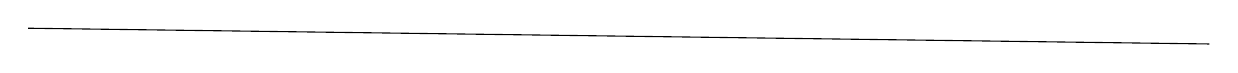
\begin{tikzpicture}\draw (0,.2)--(15,0);\end{tikzpicture}}
\deleted{$\unsure{E_{0S}}$}\quad\deleted{$\unsure{\varphi}$}
\diagram{\begin{tikzcd}[column sep=small,row sep=small]
S_0\arrow[r,dash]\arrow[d,dash]&S\arrow[d,dash]\\
k\arrow[r,dash]&W
\end{tikzcd}}
$F_S\qquad\deleted{F_S^*}\lambda\qquad\deleted{\unsure{\sigma_{E_S}}}$
\diagram{\begin{tikzcd}[column sep=small,row sep=small]
S\arrow[rr,dash,bend left,"F_S"]\arrow[d,dash]&&S\arrow[d,dash]\\
\operatorname{Spec}(W)\arrow[rr,"F_W"]\arrow[dr,dash]&&\operatorname{Spec}(W)\arrow[dl,dash]\\
&\operatorname{Spec}\mathbb Z_p&
\end{tikzcd}}
\[M=E_W\qquad E\text{ module libre de t.f.}\]
\[\deleted{F_S^*(E_W)=E_W^\sigma}\qquad\unsure{E^{\sigma'}}\]
\diagram{\begin{tikzcd}[column sep=small,row sep=small]
F_S^*(E_S)\arrow[r,"F_M"]&E_S\\
E_S\arrow[u,phantom,"\wr"]\arrow[ur,"\Phi"']&
\end{tikzcd}}
$\Phi$ \uuline{induit un isom} après $\otimes_{\mathbb Z_p}\mathbb Q_p$
\[
\unsure{A}\in\Gamma(\widehat\Omega^1_{S/W}\otimes\operatorname{End}(E_S))
\]
\[
\unsure{A'}=F_S^*(\nabla)\in\Gamma\left(\widehat\Omega^1_{S/W}\otimes\underbrace{\operatorname{End}(F_S^*(E_S))}_{\wr\ \operatorname{End}(E_S)}\right)
\]
\deleted{$\unsure{\Phi}$}\qquad\deleted{$\Phi\circ\nabla$}
\[
\Phi\circ A^\sigma=d\Phi+A\circ\Phi
\]
i.e.
\[\boxed{d\Phi=\Phi\circ A^\sigma-A\circ\Phi}\]
\margin{exprime que $F_M$ est compatible à la connexion}
\deleted{$K(A)=$}
\[\boxed{dA+[A,A]=0}\]
\margin{exprime que \inserted{la connexion} $\nabla$ définie par $A$ est à courbure nulle}
\deleted{$\Phi^{-1}$}
\[
\exists\Psi:E_S\mathbin{-}E_S,\quad\text{et }i,\text{ tel que}
\]
\[\boxed{\Psi\Phi=p^i\mathrm{id}}\]
\mspage{28}
\scanpage{30}
\figure{\begin{tikzpicture}[scale=.82]
\draw (3.2,6.6) ellipse (2.25 and 1.9);
\draw (3.15,6.58) ellipse (2.32 and 1.96);
\draw (1.6,7.0) .. controls (4.1,9.2) and (5.0,8.2) .. (2.1,6.5) .. controls (1.0,5.7) and (4.8,8.1) .. (4.2,7.4) .. controls (3.6,6.5) and (1.8,5.5) .. (2.9,5.9) .. controls (5.7,7.5) and (4.6,6.3) .. (3.2,5.6) .. controls (2.2,4.7) and (5.9,7.0) .. (4.9,5.8) .. controls (3.6,4.4) and (4.1,5.3) .. (5.0,5.8);
\draw (3.5,6.7) ellipse (.32 and .38);\fill (3.47,6.7) circle (.025);
\node at (3.55,6.68) {$V$};\node at (3.94,6.94) {$U$};
\node at (1.5,8.55) {$\unsure{\phi_m}$};\node at (3.0,7.65) {$\unsure{\phi_n}$};
\node at (5.8,8.3) {$C^1$};\node at (7.2,7.2) {$\unsure{C^{n}}$};
\node[draw,ellipse] at (9.05,8.35) {$C^0$};\node at (10.4,8.3) {$\unsure{\Phi}$};
\draw (11.2,6.15) ellipse (.68 and .53);\draw (11.18,6.1) ellipse (.73 and .42);
\draw[->] (11.85,6.2)--(10.35,6.15);\draw (10.4,6.13)--(11.7,6.05)--(10.5,6.2);
\draw (5.45,6.95).. controls (8,6.8) and (9.6,5.9)..(11.6,6.35);
\draw[->] (8.7,4.9).. controls (8.0,5.6) and (6.1,6.3)..(4.95,6.25);
\draw (6.5,2.6).. controls (7.8,5.0) and (9.8,6.0)..(11.65,6.35);
\draw (12.95,7.1).. controls (12.4,6.1) and (12.5,5.3)..(13.05,4.6);
\node at (12.15,5.15) {$\unsure{m^1}$};\node at (6.4,4.9) {$\unsure{m-n}$};
\draw[->] (3.5,6.3)--(3.4,3.6);\node at (3.1,4.55) {$\sigma$};
\draw (3.7,3.9)--(3.7,2.8)--(5.0,2.35);\draw (3.7,2.8)--(2.2,1.5);
\draw (2.5,1.65)--(4.2,2.5);\draw (2.6,1.45)--(4.3,2.3);\draw (2.8,1.3)--(4.35,2.1);
\node at (4.15,3.75) {$R^{\unsure{m}}$};\node at (4.1,1.5) {$R^{\unsure{n}}$};
\draw (.4,2.2).. controls (.1,3.1) and (1.0,3.8)..(2.0,4.1);
\draw (.3,3.35)--(.65,2.4);\draw (.65,3.7)--(.95,2.65);\draw (1.0,4.0)--(1.3,3.05);\draw (1.3,4.0)--(1.6,3.25);
\draw (9.4,2.8) ellipse (3.8 and 1.7);\draw (9.7,3.4) ellipse (2.65 and .8);
\node at (9.65,3.4) {$\sigma(V)=\sigma(U)\cap R^n$};
\node at (8.75,2.2) {$A_0=\{(\sigma_i,(U_i,V_i))\}$};\node at (12.0,2.3) {$C^n$};
\draw (8.6,2.2) ellipse (3.0 and .8);
\end{tikzpicture}}

\figure{\begin{tikzpicture}\node[draw,ellipse,inner xsep=15pt,inner ysep=6pt] {$1)$ Familles connexes $C^r$, $r\geq0$};\end{tikzpicture}}
\[V_i\subset U_i\]
$2)$ Familles régulières (quasi-régulières), $C^r$, $r\geq1$
\[
\left.\begin{array}{ll}
3)\ \text{Familles naturelles},&r\geq1\\
4)\ \text{Familles normales},&r\geq1
\end{array}\right\}\ C^{r-1}
\]
\figure{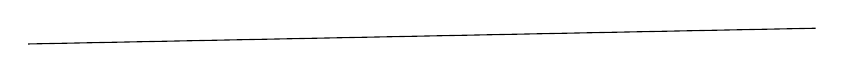
\begin{tikzpicture}\draw (0,0)--(10,.2);\end{tikzpicture}}
\figure{\begin{tikzpicture}\node[draw,ellipse,inner sep=8pt] {$(\sigma_1,(U_1,V_1))\qquad(\sigma_2,(U_2,V_2))$};\end{tikzpicture}}

$1)$ $V_1\cap V_2\ne\varnothing$

$2)$ $(\sigma'_1,(U_1\cap U_2,V_1\cap V_2))$

\hspace{2em}$(\sigma'_2,(U_1\cap U_2,V_1\cap V_2))$

\figure{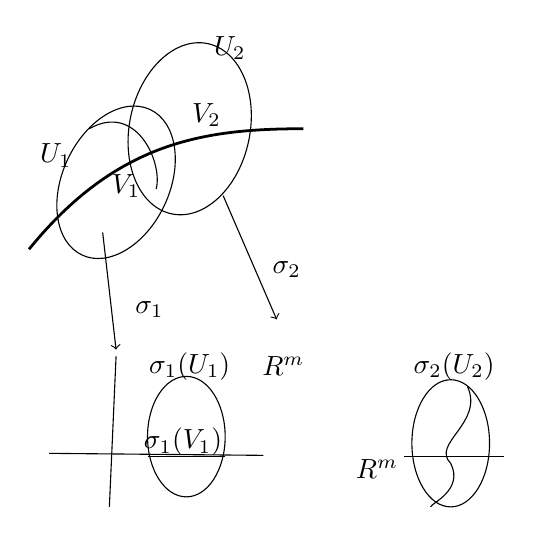
\begin{tikzpicture}[scale=.85]
\draw[rotate around={-25:(3,5.4)}] (3,5.4) ellipse (.8 and 1.2);
\draw[rotate around={-12:(4.1,6.2)}] (4.1,6.2) ellipse (.9 and 1.3);
\draw[line width=1pt] (1.7,4.4).. controls (3.0,6.0) and (4.3,6.2)..(5.8,6.2);
\draw (2.6,6.2)..controls (3.3,6.6) and (3.7,5.7)..(3.6,5.3);
\node at (2.1,5.8) {$U_1$};\node at (4.7,7.4) {$U_2$};\node at (3.15,5.35) {$V_1$};\node at (4.35,6.4) {$V_2$};
\draw[->] (2.8,4.65)--(3.0,2.9);\node at (3.5,3.5) {$\sigma_1$};
\draw[->] (4.6,5.2)--(5.4,3.35);\node at (5.55,4.1) {$\sigma_2$};
\draw (3.0,2.8)--(2.9,.55);\draw (2.0,1.35)--(5.2,1.32);
\draw (4.05,1.6) ellipse (.58 and .9);\draw (3.47,1.3)--(4.63,1.3);
\node at (4.1,2.65) {$\sigma_1(U_1)$};\node at (4.0,1.52) {$\sigma_1(V_1)$};\node at (5.5,2.65) {$R^m$};
\draw (7.3,1.3)--(8.8,1.3);\draw (8.0,1.5) ellipse (.58 and .95);
\draw (8.25,2.35)..controls (8.5,1.8) and (7.7,1.5)..(8.0,1.2)..controls (8.2,.8) and (7.7,.6)..(7.7,.55);
\node at (8.05,2.65) {$\sigma_2(U_2)$};\node at (6.9,1.12) {$R^m$};
\end{tikzpicture}}
\figure{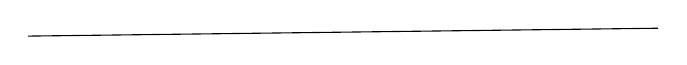
\begin{tikzpicture}\draw (0,0)--(8,.1);\end{tikzpicture}}
\[
U_1\cap V_2=V_1\cap V_2
\]
\[
U_2\cap V_1=V_1\cap V_2
\]
\mspage{29}
\scanpage{31}
$M=E_S\overset u{\mathbin{-}}E'_S=M'$ compatible aux $\nabla_M$, \inserted{$\nabla_{\unsure{N|M'}}$,} $F_M$, $F_{\unsure{N|M'}}$ ?
\[u\circ A=du+A'\circ u\]
\[\boxed{du=u\circ A-A'\circ u}\]
\diagram{\begin{tikzcd}[column sep=large,row sep=large]
E_S\arrow[r,"u"]&E'_S\\
E_S\arrow[u,"F_M"]\arrow[r,"F_S^*(u)=u^\sigma"']&E'_S\arrow[u,"F_{M'}"']
\end{tikzcd}}
\[\boxed{F_{M'}u^\sigma=uF_M}\]

\uline{Ex}\qquad\uline{Modules inversibles}. Alors
\[
\Phi=\varphi\in\Gamma(\underline O_S)\qquad A=\omega\in\Gamma(\widehat\Omega^1_{S/W})
\]
\[
\boxed{\begin{aligned}
d\varphi&=\varphi(\omega^\sigma-\omega)\\
d\omega&=0\\
\varphi\psi&=p^{\unsure{\nu}}
\end{aligned}}
\]
Si on a un \unsure{second} $(\varphi',\omega')$, ils sont isom ssi
\[
\exists\ u\in\Gamma\underline O_S^*\quad\text{satisfaisant}
\]
\deleted{$\unsure{d\log u}=\unsure{\omega'-\omega}$}\inserted{$\deleted{\frac{du}{u}}$}
\[
\boxed{\left\{\begin{aligned}
\omega'-\omega&=-\frac{du}{u}\\
\varphi'/\varphi&=u/u^\sigma
\end{aligned}\right.}
\]
Donc, classification est donnée par \unsure{les classes de cohomologie du}
\diagram{\begin{tikzcd}[column sep=small,row sep=large]
\Gamma(\underline O_S^*)\arrow[r]&\Gamma(\deleted{\unsure{2}}\widehat\Omega^1_{S/W})\times\Gamma(\underline O_S)^!\arrow[r]&\Gamma(\Omega^2_{S/W})\times\Gamma(\Omega^1_S)[1/p]\\
u\arrow[r,mapsto]&\left(\frac{du}{u},u/u^\sigma\right)&\\
&(\varphi,\omega)\arrow[r]&\left(d\omega,\frac{d\varphi}{\varphi}-(\omega^\sigma-\omega)\right)
\end{tikzcd}}
\margin{\unsure{éléts} inversibles dans $A[1/p]$}
\mspage{30}
\scanpage{32}
\mspage{31}
\mspage{55 ter}

\uline{Démonstration.} Le cas a) n'est autre que 5.10 et a été mis pour mémoire.

b) \deleted{\unsure{Le cas $\ell\ne p$ n'est autre que le critère galoisien de ré}}\inserted{La première assertion est une conséquence \deleted{\unsure{immé}} triviale de} a) et des définitions. Pour prouver la dernière assertion dans b), on peut \deleted{donc} supposer que $\ell\ne p$, mais alors grâce à a) il suffit de prendre pour K' une extension finie séparable de K correspondant à un sous-groupe ouvert $\pi'$ de $\pi=\operatorname{Gal}(\bar K/K)$ dont l'intersection avec le groupe d'inertie I est contenue dans le \deleted{\unsure{stabi}} noyau de la représentation de I sur $T_\ell(A_K(\bar K))$, lequel est \deleted{\unsure{fi}} ouvert par hypothèse (cf. 5.12.1).

c) On a déjà signalé que $1)\Rightarrow2)$ (5.12.2), il est trivial que $2)\Rightarrow3)$, reste à prouver que $3)\Rightarrow1)$. Pour $\ell\ne p$, ce n'est autre que \inserted{le} critère galoisien de réduction semi-stable 3.5. Pour $\ell=p$, on peut procéder ainsi. Choisissons un nombre premier $\ell'\ne p$, et appliquons à celui-ci les considérations de 4.1. \deleted{On est donc ramené à prouver que la représentation} Supposons S strictement local, ce qui est loisible (3.4.0), prenons une extension galoisienne finie K' de K, de groupe G, telle que $A_{K'}$ ait réduction semi-stable. Il faut prouver que la représentation de G sur les trois quotients intervenant dans (4.1.1) est triviale, ou ce qui revient au même, que la \deleted{somme des traces} représentation somme est triviale, ou encore, que la trace de cette dernière est ``triviale'', i.e. constante . Or nous avons vu dans 4.3 a) que cette fonction trace est indépendante \unsure{da|de} choix de $\ell'\ne p$, et dans 6.\unsure{4} plus bas nous indiquons une méthode de calcul de cette fonction en \deleted{fonction}\inserted{termes} de $T_p(A_K)$ également. Ce calcul donne trivialement une fonction constante dans le cas où $T_p(A_K)$ a bonne réduction virtuelle, et cela achève la démonstration.

\uline{Remarque} 5.13.1. Il semble plausible que si $X_\eta$ est un \inserted{pro-$\ell$-} groupe de Barsotti-Tate sur $\eta$ qui a bonne réduction virtuelle sur S, et bonne réduction virtuelle essentielle d'échelon n, alors il a bonne réduction virtuelle d'échelon n. (C'est \deleted{\unsure{ce qui avait été utilisé, pour}} vrai pour $\ell\ne p$.)
\scanpage{34}
\mspage{33}

Détermination du module de Dieudonné filtré du groupe de Lubin-Tate.

$K$ extension finie de $\mathbb Q_p$, anneau d'entiers $A$, corps résiduel
\[
k\simeq\mathbb F_q,\quad q=p^f,\qquad [K:\mathbb Q_p]=h=ef,\qquad \pi\in A\quad\text{uniformisante}.
\]
\diagram{\begin{tikzcd}
\mathbb Z_p \arrow[r,dash] \arrow[d,dash] & A \arrow[d,dash]\\
\mathbb Q_p \arrow[r,dash] & K
\end{tikzcd}}

$W=W_\infty(k)$ vecteurs de Witt,
\diagram{\begin{tikzcd}
\mathbb Z_p \arrow[r,hook,"{(f)}"'] & W \arrow[r,hook,"i","{(e)}"'] & A
\end{tikzcd}}

On veut déterminer \inserted{d'abord} les grps de B.T. \inserted{$G_0$} (de hauteur ($=\unsure{\mathrm{rang}}$)) $h$ sur \deleted{$\unsure{\mathbb F_q}$} $k$, avec opération de $A$ dessus $[$telle que
\[
\pi_{G_0}=F^f\quad\text{(endomorphisme de Frobenius de $G_0/\mathbb F_q$)}\,].
\]
Par la théorie de Dieudonné, ils correspondent aux modules libres \inserted{$M$} de rang $h$ sur $W$, avec endom $\sigma$-linéaire ($\sigma$ autom de Frob. de $W$) $F_M$, et opération de $A$ sur $M$ ($\lambda\mapsto\lambda_M$) par $W$-\unsure{autom|endom} commutant à $F_M$, satisfaisant
\[
\bigl[\ (*)\quad\deleted{\unsure{\pi_M}}\ F_M^f=\pi_M\ \bigr]
\]
\margin{$(*')\ \exists V_M$ t.q. $F_MV_M=V_MF_M=p$}
\diagram{\begin{tikzcd}
A \arrow[r,dash] \arrow[d,dash] & A\otimes_{\mathbb Z_p}W \arrow[d,dash]\\
\mathbb Z_p \arrow[r,dash] & W
\end{tikzcd}}

Les deux structures de module sur $M$ correspondent à une structure de module sur $A_W=A\otimes_{\mathbb Z_p}W$. Soit \deleted{$\unsure{\sigma_W}$} $\sigma_A$ l'autom de $A_W=A\otimes_{\mathbb Z_p}W$ donné par
\[
\sigma_A(\lambda\otimes w)=\lambda\otimes\sigma w.
\]
Alors la donnée de $F_M$ équivaut à la donnée d'un endom $\sigma_A$-linéaire, satisfaisant $(*)$ $(*')$.
\scanpage{35}
\mspage{34}
\mspage{84}
\margin{n° 382}

application de classe $C^{r-k}$ de $f^{-1}P^k(X',\varpi')=X\times_{X'}P^k(X',\unsure{\varphi'|\varpi'})$ dans $P^k(X,\varpi)$, qui, si X, X', Y' sont des variétés pures, est un morphisme pour les fibrations sur X.

7.2.7. Soient X, Y des variétés de classe $C^r$, $\varphi:X\longrightarrow Y$ une submersion, E un fibré vectoriel de classe $C^r$ sur Y, et E' le fibré vectoriel image réciproque de E suivant $\varphi$. Soit k un entier fini $\leq r$ et soit $P^k(Y,E)_0$ le fibré vectoriel sur Y dont la fibre $P_y^k(Y,E)_0$ en $y\in Y$ est l'espace des jets de sections nulles en y. Soient $x\in X$ et $y=f(x)$. On a un morphisme canonique de $P_x^k(X)\otimes\varphi^{-1}P_y^k(Y,E)_0$ dans $P_x^k(X,E')$, dont l'image est l'ensemble des jets de section de E' en x dont la restriction à $X_y=\varphi^{-1}(y)$ est nulle, et une suite exacte de morphismes d'espaces fibrés vectoriels
\diagram{\begin{tikzcd}
P^k(X)\otimes\varphi^{-1}(P^k(Y,E)_0) \arrow[r] & P^k(X,E') \arrow[r] & P^k(X/Y,E) \arrow[r] & 0.
\end{tikzcd}}
La fibre de $P^k(X/Y,E)$ située sur x s'identifie à $J_x^k(X_y,E_y)$, où $E_y$ est la fibre de E sur y.

Soient encore Y' une variété pure de classe $C^k$, $f:Y'\longrightarrow Y$ un morphisme de Y' dans Y, et $X'=Y'\times_Y X$ le produit de X et Y' au-dessus de Y. Alors l'application canonique $\varpi':X'\longrightarrow Y'$ est une submersion $(\qquad\qquad)$ et l'on a
\[
P^k(X'/Y',f^{-1}E)=P^k(X/Y,E)\otimes_{Y'}X'.
\]

7.2.8. Soient X, Y des variétés de classe $C^r$, $\varpi:Y\longrightarrow X$ une submersion, $r'\leq r$ et k un entier fini $\leq r'$, et soient Y', X' les variétés de classe $C^{r'}$ obtenues à partir de Y, X par affaiblissement de structure $(\qquad\qquad)$. Alors $P^k(X',\varpi)$ est obtenue par affaiblissement de structure de $C^{r-k}$ à $C^{r'-k}$ à partir de $P^k(X,\varpi)$.
\scanpage{36}
\mspage{35}

On a $A\otimes_{\mathbb Z_p}W$ étale sur $A$, ext. résiduelle
\[
k\otimes_{\mathbb F_p}k\simeq k^\Sigma,\qquad\Sigma=\operatorname{Aut}k=\operatorname{Aut}W,
\]
\[
A\otimes_{\mathbb Z_p}W\simeq A^\Sigma,\qquad \Sigma\simeq\mathbb Z/f\mathbb Z
\]
en correspondance bijection canonique avec $[0,f-1]$ par $\nu\mapsto\sigma^\nu$\quad\deleted{$(\unsure{\sigma\lambda=\lambda^p})$}.

On a
\[
\sigma_A(x_0,x_1,\ldots,x_{f-1})=(x_1,\ldots,x_{f-1},x_0).
\]
La donnée d'un module \inserted{\unsure{libre}} $M$ \inserted{sur $A\otimes_{\mathbb Z_p}W$} équivaut à la donnée de modules $(M_\nu)_{\nu\in\Sigma}$ sur $A$; le rang de $M$ est la somme des rangs des $M_\nu$ \inserted{(on le veut égal à $h$)}. La donnée d'un endom $F_M$ $\sigma_A$-linéaire équivaut à la donnée d'hom. $A$-linéaires
\diagram{\begin{tikzcd}
M_0 \arrow[r,"\varphi_0"] & M_1 \arrow[r,"\varphi_1"] & \cdots \arrow[r] & M_{f-1} \arrow[r,"\varphi_{f-1}"] & M_0
\end{tikzcd}}
La condition $(*)$ \deleted{\unsure{s'écrit}} implique que les $f$ composés circulaires sont des isogénies, donc les $\varphi_i$ sont injectifs, donc les $\varphi_i$ des isogénies (car les rangs des $M_\nu$ tous égaux $\ldots$). \deleted{Donc} --- Utilisant maintenant le fait que la somme des rangs des $M_\nu$ est $h$, on trouve que les $M_\nu$ sont inversibles.
\margin{ce serait aussi une \unsure{conséquence} de \deleted{$(*')$} $(*)$ \unsure{et de|avec} $\pi$ un élét non nul \uline{quelconque} de $A$}

\deleted{On peut alors trouver un unique module \unsure{inversible} $\Omega$ sur $A$,}
On peut alors identifier tous les $M_\nu$ à \deleted{$M_0=\unsure{\Omega}$,} $M_0=\unsure{\mathfrak t}$, \deleted{\unsure{grâce à}} en choisissant \deleted{\unsure{comme}} pour \unsure{tt $\nu$}, l'isom \inserted{$0\leq\nu\leq f-1$}
\[
M_0\overset\sim\longrightarrow M_{\unsure{i|\nu}}
\]
donné par
\[
\pi^{-m_\nu}(\varphi_{\nu-1}\varphi_{\nu-2}\cdots\varphi_0),
\]
où $m_\nu$ est un entier $\geq0$ uniquement déterminé $(0\leq m_0\leq m_1\leq\cdots\leq m_{f-1})$. On trouve donc un isom can.
\[
M\simeq\Omega\otimes_{\mathbb Z_p}W=\Omega\otimes_A(A\otimes_{\mathbb Z_p}W).
\]
\scanpage{37}
\mspage{36}
\mspage{83}
\margin{n° 382}

des germes en x de sections qui ont un contact d'ordre $\geq k'$ avec la section nulle ; cet espace est la fibre en x d'un sous-fibré vectoriel de $P^k(X,E)$, qui est aussi un module sur $P^k(X)$. En particulier, le noyau de $P^k(X,E)\longrightarrow P^{k-1}(X,E)$ s'identifie au produit tensoriel $S^k(T(X)^*)\otimes E$ de E avec la k-ième puissance symétrique du dual du fibré tangent à X.

7.2.4. Soient X, Y des variétés de classe $C^r$, $\varpi:Y\longrightarrow X$ une submersion, $k'\leq k$ des entiers finis $\leq r$, $\ell=k-k'$, et soit $\varpi_1$ la projection de $P^{k'}(X,\varpi)$ sur X. L'application canonique de $J^k(X,Y)$ dans $J^\ell(X,J^{k'}(X,Y))$ définie au n° 7.1.10 induit une application de classe $C^{r-k}$ de $P^k(X,\varpi)$ dans $P^\ell(X,\varpi_1)$ qui, lorsque K est de caractéristique zéro, est un isomorphisme de $P^k(X,\varpi)$ sur une sous-variété de $P^\ell(X,\varpi_1)$ ; cette application est un morphisme de fibrés sur X si X et Y sont des variétés pures.

7.2.5. Soient X, Y, Y' des variétés de classe $C^r$, $\varpi:Y\longrightarrow X$ et $\varpi':Y'\longrightarrow X$ des submersions, $g:Y\longrightarrow Y'$ un morphisme de Y dans Y' tel que $\varpi'\circ g=\varpi$, \inserted{(1) et k un entier $\leq r$. L'application $j^k(\mathrm{id}.,g)$} (cf. n° 7.1.11) induit une application $P^k(g):P^k(X,\varpi)\longrightarrow P^k(X,\varpi')$ de classe $C^{r-k}$ qui, lorsque X, Y, Y' sont des variétés pures, est un morphisme pour les fibrations sur X. Si $Y''$ est une variété de classe $C^r$, $\varpi'':Y''\longrightarrow X$ une submersion et $g':Y'\longrightarrow Y''$ un morphisme tel que $\varpi'=\varpi''\circ g'$, alors $P^k(g'\circ g)=P^k(g')\circ P^k(g)$. Si $E\xrightarrow{\lambda}F\xrightarrow{\mu}G$ est une suite exacte de fibrés vectoriels sur X, alors
\diagram{\begin{tikzcd}
P^k(X,E) \arrow[r,"P^k(\lambda)"] & P^k(X,F) \arrow[r,"P^k(\mu)"] & P^k(X,G)
\end{tikzcd}}
est une suite exacte. Si A et B sont des fibrés vectoriels sur X, alors
\[
P_x^k(X,A\otimes B)\simeq P_x^k(X,A)\otimes_{P_x^k(X)}P_x^k(X,B),\quad\text{pour tout }x\in X.
\]

7.2.6. Soient X, X', Y' des variétés de classe $C^r$, $f:X\longrightarrow X'$ un morphisme, $\varpi:Y'\longrightarrow X'$ une submersion, $Y=X\times_{X'}Y'$ (n° 4.11.3) et $\varpi$ la submersion canonique de Y sur X, $(\qquad)$. L'application $j^k(f,\mathrm{Id}.)$ (cf. n° 7.1.11) induit une
\scanpage{38}
\mspage{37}

\deleted{Alors \unsure{et} $F_M$ est donné par les entiers $m_i$ \inserted{et par $\varphi_{f-1}$}, \unsure{variant avec les $m_i,m_{i-1}$}.}

On a choisi les isom de telle façon que les $\varphi_\nu$ $(0\leq\nu\leq f-2)$ sont de la forme
\[
\varphi_\nu=\pi^{r_\nu}\operatorname{id}_\Omega\qquad(r_\nu\geq0\deleted{\unsure{)}},\ 0\leq\nu\leq f-2)
\]
et $\varphi_{f-1}$ est donné alors par
\[
\varphi_{f-1}=\lambda\operatorname{id}_\Omega\qquad\lambda\in A,\quad\inserted{\text{soit}}\ \lambda=\pi^{r_{f-1}}u,\ u\in A^*.
\]
\deleted{\unsure{Donc}} On a donc
\[
F_M^f=\pi^{r_0+\cdots+r_{f-2}+r_{f-1}}u=\varpi\qquad u\in A^*.
\]
\deleted{On a encore
\[
M/F_MM\simeq A/\pi^{\unsure{r_{f-1}}}A+A/\pi^{\unsure{r_i}}A+\cdots+A/\pi^{r_{f-2}}A.
\]}
La condition $(*)'$ s'écrit
\deleted{\unsure{donc}\quad$\unsure{\operatorname{dim}G_K}$}
\[
\begin{array}{l}
p\ \text{divisible par }\pi^{r_\nu}\ \text{pour tt }0\leq\nu\leq f-2,\\
\hspace{4em}\text{par }u\pi^{r_{f-1}}
\end{array}
\]
i.e.
\[
\left\{\begin{array}{l}
\boxed{\deleted{0\leq}\ r_\nu\leq e}\quad\text{pour }0\leq\nu\leq f-1\\
\boxed{\deleted{\unsure{r_{f-1}+v(u)\leq e}}}
\end{array}\right.
\]
On a
\[
M/F_MM=A/u\pi^{r_{f-1}}A+A/\pi^{r_0}A+\cdots+A/\pi^{r_{f-2}}A
\]
est de \deleted{\unsure{hauteur}} longueur
\[
\boxed{\dim G_0=\deleted{\unsure{v(\varpi)}}\inserted{\unsure{\operatorname{long}A/(\varpi A)}\ \deleted{\unsure{f}}}=r_0+\cdots+r_{f-2}+(r_{f-1}\deleted{\unsure{+v(u)}})}
\]
\[
(\leq fe=h).
\]

\deleted{Supposons maintenant}
\unsure{Donc on trouve}
\[
\boxed{\begin{gathered}
\dim G_0=1\Longleftrightarrow F_M^f\ \deleted{\text{une}}\inserted{=\varpi_M,\ \varpi\ \text{une}}\ \text{\uline{uniformisante} de }A\\
\text{(qu'on peut supposer alors }=\pi,\ \text{quitte à changer }\pi\text{ !)}\\
\Longleftrightarrow\text{tous les }r_\nu\text{ sauf un seul}\inserted{r_{\nu_0}}\text{ sont nuls, }r_{\nu_0}=1,\ u\ \text{une unité}
\end{gathered}}
\]
\margin{$(\uline{u=1\text{ si}}\ \text{on veut }\varpi=\pi)$}

\unsure{C}
\scanpage{39}
\mspage{38}
\mspage{82}
\margin{n° 382}

variétés sont pures, et si $X'=X$, (resp. $Y'=Y$), l'application $j^k(\mathrm{Id}.,g)$ (resp. $j^k(f,\mathrm{Id}.)$) est un morphisme pour les fibrations sur X (resp. sur Y).

7.1.12. Soient X, Y des variétés de classe $C^r$, $r'\leq r$ et k un entier fini $\leq r'$. Soient X' et Y' les variétés de classe $C^{r'}$ obtenues à partir de X et Y par affaiblissement de structure (n° 4.13.1). Alors $J^k(X',Y')$ est obtenue par affaiblissement de structure de $C^{r-k}$ à $C^{r'-k}$ à partir de $J^k(X,Y)$.

7.2 - \uline{Jets de sections.}

7.2.1. Soient X, Y des variétés de classe $C^r$, $\varpi:Y\longrightarrow X$ une submersion et $k\leq r$. On note $P_x^k(X,\varpi)$ l'ensemble des éléments f de $J_x^k(X,Y)$ tels que $j_y^k(\varpi)\circ f$ soit le jet de l'application identique de X, y étant le but de f. Le jet f a cette propriété si et seulement si c'est le jet d'ordre k d'un germe en x d'application f de X dans Y tel que $\varpi\circ f$ soit le germe de l'application identique.

7.2.2. On suppose dorénavant k fini. L'ensemble $P_x^k(X,\varpi)$ est une sous-variété fermée de $J_x^k(X,Y)$, et la réunion $P^k(X,\varpi)$ des $P_x^k(X,\varpi)$ $(x\in X)$ est une sous-variété fermée de $J^k(X,Y)$. Si X et Y sont des variétés pures, les fibrations de $J^k(X,Y)$ sur $X\times Y$, X et Y (cf. n° 7.1.6) induisent des fibrations de $P^k(X,\varpi)$, de bases respectives $\varpi(X)\times Y$, $\varpi(X)$ et Y. Si $\varpi$ est la projection d'une fibration $\xi$, on écrira aussi $P^k(X,\xi)$ pour $P^k(X,\varpi)$. Si $\varpi$ est la projection d'un fibré vectoriel E, alors $P^k(X,\varpi)$ est un fibré vectoriel sur X, et un fibré en modules sur le fibré en algèbres $P^k(X)$ ; on le notera aussi $P^k(X,E)$. Si de plus E est le fibré vectoriel trivial $F_X$ de fibre F sur X, alors
\[
P^k(X,\varpi)\simeq P^k(X)\otimes F_X\simeq J^k(X,F).
\]

7.2.3. Soit encore k' un entier $\leq k$. L'application $J^k(X,Y)\longrightarrow J^{k'}(X,Y)$ (cf. n° 7.1.2) induit une application $P^k(X,\varpi)\longrightarrow P^{k'}(X,\varpi)$ qui est un morphisme pour les fibrations sur X. Si Y = E est un fibré vectoriel sur X, le noyau du morphisme $P_x^k(X,E)\longrightarrow P_x^{k'}(X,E)$ $(x\in X)$ s'identifie à l'espace vectoriel des jets
\scanpage{40}
\mspage{39}

Donc \deleted{\unsure{le}} on trouve

\uline{Proposition} $A$, \inserted{$k$,} $W,e,f$, \inserted{$h=ef$,} comme plus haut, $G_0$ un grp de B.T. \inserted{de hauteur $h$} sur \deleted{$A$} $k$ sur lequel $A$ opère, \deleted{\unsure{Alors $F$}} $M$ son module de Dieudonné (module libre de rang $h$ sur $W$).
$F_{G_0}^f$ est de la forme $\varpi_{G_0}$, où $\varpi\in A$, et on a $\dim G_0=\operatorname{long}A/\varpi A=v(\varpi)$.
Alors \deleted{conditions équivalentes} conditions équivalentes
\[
\begin{array}{ll}
\text{(i)}&\dim G_0=1\\
\text{(ii)}&F_{G_0}^f=\pi_{G_0},\quad\pi\ \text{une \uline{uniformisante} de }A\ \text{(uniqt déterminée !)}
\end{array}
\]
(iii) Le module de Dieudonné $M$ de $G_0$ \inserted{(sur $W$,)} avec $F_M$ et opération de $A$, est donné par un triple $(\Omega,\unsure{\nu_0|\nu},\pi)$ où $\Omega$ est un module inv. sur $A$, $0\leq\unsure{\nu_0|\nu}\leq f-1$, $\pi$ une uniformisante de $A$ par
\[
\left\{\begin{aligned}
M&=\Omega\otimes_{\mathbb Z_p}W\simeq\Omega\otimes_A(A\otimes_{\mathbb Z_p}W)\\
F_M&=\operatorname{id}_\Omega\otimes_{\mathbb Z_p}\sigma+\operatorname{pr}_\nu[(\pi-1)\otimes\sigma]\deleted{\unsure{\operatorname{pr}_\nu}}
\end{aligned}\right.
\]
\margin{(isom de $A\otimes_{\mathbb Z_p}W$-mod)}
où $\operatorname{pr}_\nu$ est la \deleted{\unsure{facteur}} projection de $M$ sur son $\nu$-ième facteur \inserted{$M_\nu$} (correspondant à la décomposition $A\otimes_{\mathbb Z_p}W\simeq A^{[0,f-1]}$).

\margin{\uline{NB} Tous ces groupes (pour $\nu$ variable) sont déduits de l'un d'entre eux (disons $\nu=0$) par \unsure{transformation} à l'aide des $f$ automorphismes de $k\simeq\mathbb F_q=\mathbb F_{p^f}$.}

\uline{NB} Revenons au cas général, où on ne suppose pas néc. $\dim G_0=1$ \inserted{(mais $G_0$ de hauteur $h\ldots$)}. Soit $G'_0$ défini comme $G_0$ par $\Omega'$, et les $r'_\nu$ $(0\leq\nu\leq f-1)$ $u'\in A^*$. On cherche les homs compatibles avec l'action de $A$ de $G_0$ dans $G'_0$, i.e. les hom de $A\otimes_{\mathbb Z_p}W$-modules de $M'$ dans $M$, compatibles avec $F_M,F_{M'}$. On trouve facilement que pour qu'il existe un tel hom qui soit $\ne0$ ($\Longleftrightarrow$ une isogénie), il f. et suffit qu'on ait $\varpi=\varpi'$ i.e. $F_{G_0}^f=F_{G'_0}^f$ (dans $A$). Dans ce cas, le groupe des homs en question, comme $A$-module, est isom au \deleted{\unsure{$E'$}} sous-module
\[
H\subset\operatorname{Hom}(\Omega',\Omega)
\]
formé des $v_0:\Omega'\longrightarrow\Omega$ tels que \inserted{pour tt $0\leq\nu\leq f-2$} on ait
\[
v_0\pi^{(\sum_0^\nu r_i)-(\sum_0^\nu r'_i)}\in\operatorname{Hom}(\Omega',\Omega)
\]
i.e.
\[
\operatorname{val}(v_0)+\sum_0^\nu r_i-\sum_0^\nu r'_i\geq0.
\]
\scanpage{41}
\mspage{40}
\mspage{81}
\margin{n°382}

$f\in J^k(X,K^q)_0$).

7.1.7. Si Y = K, la structure d'algèbre des $P_x^k(X)$ munit $P^k(X)$ d'une structure d'espace fibré vectoriel en algèbres de base X, de classe $C^{r-k}$.

7.1.8. Soit X une variété de classe $C^r$, et soit $x\in X$. L'espace vectoriel $J_0^1(K,X)_x$ s'identifie canoniquement à l'espace tangent $T_x(X)$ à X en x. La réunion $T(X)=\bigcup_{x\in X}T_x(X)$ des espaces tangents aux points de X s'identifie canoniquement à $J^1(K,X)$, et admet donc une structure d'espace fibré vectoriel sur X, de classe $C^{r-1}$. C'est le \uline{fibré tangent} $T(X)$ à X.

7.1.9. Soient X et Y des variétés de classe $C^r$ et k un entier fini $\leq r$. Un morphisme $f:X\longrightarrow Y$ définit une application $x\longrightarrow j_x^k(f)$ de X dans $J^k(X,Y)$ qui est une section de classe $C^{r-k}$ pour la fibration de $J^k(X,Y)$ sur X. L'application $J^k(X,Y)\longrightarrow J^{k'}(X,Y)$ (k' entier $\leq k$, cf. n° 7.1.2) est un morphisme pour les fibrations sur X et pour les fibrations sur Y.

7.1.10. Soient X, Y des variétés de classe $C^r$, $k'\leq k$ des entiers finis $\leq r$, $\ell=k-k'$. Soit f une application de classe $C^r$, dans Y, d'un ouvert U de X. L'application $x\longrightarrow j^{k'}(f)$ de U dans $J^{k'}(X,Y)$ est de classe $C^{r-k'}$ et son jet d'ordre $\ell$ en x ne dépend que de $j^k(f)$. On obtient ainsi une application canonique de classe $C^{r-k}$ de $J^k(X,Y)$ dans $J^\ell(X,J^{k'}(X,Y))$ qui, si K est de caractéristique zéro, est un isomorphisme de $J^k(X,Y)$ sur une sous-variété de $J^\ell(X,J^{k'}(X,Y))$ et qui, si X et Y sont des variétés pures, est un morphisme pour les fibrations sur X.

7.1.11. Soient X, Y, X', Y' des variétés de classe $C^r$, $f:X\longrightarrow X'$ et $g:Y'\longrightarrow Y$ des morphismes, $x\in X$, $y'\in Y'$, $x'=f(x)$, $y=g(y')$. Les morphismes f et g définissent une application $j_{x'}^k(f,g)_y:J_{x'}^k(X',Y')_{y'}\longrightarrow J_x^k(X,Y)_y$ caractérisée par $u\longrightarrow P_{y'}^k\circ u\circ P_x^k(f)$. On en déduit une application, $j^k(f,g)$ de $f^{-1}J^k(X',Y')=X\times_{X'}J^k(X',Y')$ dans $J^k(X,Y)$, de classe $C^{r-k}$. Si ces
\scanpage{42}
\mspage{41}

En particulier, si $G_0,G'_0$ satisfont aux conditions de la proposition, alors $\operatorname{Hom}(G_0,G'_0)\ne0$, i.e. $G_0$ et $G'_0$ sont isogènes, ssi $\pi=\pi'$. \deleted{\unsure{Si}} S'il en est ainsi, alors \deleted{\unsure{on a}} on a
\[
\left\{\begin{array}{ll}
\text{si }\nu\unsure{\leq|<}\nu'&\deleted{G_0=G'_0},\quad\operatorname{Hom}_A(G_0,G'_0)\overset\sim\longrightarrow\operatorname{Hom}(\Omega',\Omega)\\
\text{si }\nu>\nu'&\operatorname{Hom}_A(G_0,G'_0)\simeq\pi\operatorname{Hom}(\Omega',\Omega)
\end{array}\right.
\]

\uline{Re NB} Revenons au cas général où on ne suppose pas néc. $\dim G_0=1$, \uuline{ni} \unsure{sa} hauteur $=h$. Classifions à isogénie près \deleted{\unsure{les}} ces $G_0$, donc les $M_\nu$ $(0\leq\nu\leq f-1)$ deviennent des vectoriels \deleted{de dim.}\inserted{sur le} corps $K$, isomorphes par les $\varphi_\nu$ $(0\leq\nu\leq f-2)$. Alors
\deleted{\unsure{on est en présence de}}
\[
M\simeq\Omega\otimes_{\mathbb Q_p}W=\Omega\otimes_K(K\otimes_{\mathbb Q_p}K_0)
\]
\margin{$K_0$ corps des fractions de $W$}
et $F$ est déterminé par la connaissance de $\varphi_{f-1}$, qui est un endom de $M$, soit $\varpi$, de sorte qu'on a
\[
F_M^f=\varpi\otimes_{\mathbb Q_p}\operatorname{id}_{K_0}=\varpi\otimes_K(K\otimes_{\mathbb Q_p}K_0).
\]
La condition ``d'effectivité'' en termes de $\varpi$ est
\[
\left\{\begin{array}{l}
\varpi\ \text{laisse invariant un réseau}\\
p^f\varpi^{-1}\ \text{laisse invariant un réseau}
\end{array}\right.
\]
\scanpage{43}
\mspage{42}
\mspage{79}
\margin{n° 382}

$|\alpha|\leq k$ (cf. n° 2.5.3 et 3.5.2) ; si $r\ne\omega$, ces valeurs peuvent être choisies arbitrairement.

L'ensemble $J^k(K^p,K^q)$ s'identifie canoniquement à $K^p\times K^q\times L_{p,q}^k$, où l'on a posé $L_{p,q}^k=J_0^k(K^p,K^q)_0$. L'ensemble $L_{p,q}^k$ admet une structure d'espace vectoriel sur K, caractérisée par
\[
j_0^k(f)+j_0^k(g)=j_0^k(f+g),\quad\alpha.j_0^k(f)=j_0^k(\alpha.f)\qquad(\alpha\in K),
\]
f et g étant des applications dans $K^q$ d'un voisinage ouvert de l'origine de $K^p$, de classe $C^r$, envoyant l'origine sur l'origine.

Supposons k fini. Alors $L_{p,q}^k$ s'identifie canoniquement à $K^{q,c(k,p)}$, avec $c(k,p)=\binom{k+p}{p}$, sa base canonique étant formée des parties principales d'ordre k des applications polynomiales $p_{j,\beta}:x\longrightarrow(f^1(x),\ldots,f^q(x))$, où $f^i(x)=\delta_j^i.x^\beta$ $(j=1,\ldots,q\ ;\ |\beta|\leq k)$. Cette identification est compatible avec la structure vectorielle définie précédemment. Les espaces $L_{p,q}^k$ et $J^k(K^p,K^q)$ sont ainsi munis canoniquement d'une structure de variété analytique.

L'ensemble $L_p^k$ des jets inversibles d'ordre k de $K^p$ dans $K^p$, de source et but l'origine, muni de la loi de composition des jets, est une variété de groupe de classe $C^\omega$ ; le groupe $L_p^k\times L_q^k$ opère analytiquement à gauche sur $L_{p,q}^k$ par la composition des jets :
\[
(a,b).c=a\circ c\circ b^{-1}\qquad(a\in L_p^k,\ b\in L_q^k,\ c\in L_{p,q}^k\ ;).
\]
Soit $k'\leq k$. L'application naturelle $L_{p,q}^k\longrightarrow L_{p,q}^{k'}$ (cf. 7.1.4) est surjective, linéaire. Son noyau est l'ensemble des jets d'ordre k de $K^p$ dans $K^q$ qui ont un contact d'ordre $\geq k'$ avec l'application nulle. L'application naturelle $L_p^k\longrightarrow L_p^{k'}$ est un morphisme surjectif de variétés de groupe de classe $C^\omega$.

7.1.6. Soient X et Y des variétés de classe $C^r$, k un entier fini $\leq r$ et k' un entier $\leq k$. Si $(U,\varphi,p)$ et $(V,\psi,q)$ sont des cartes de X et Y, on a des isomorphismes
\scanpage{44}
Revenons aux conditions de la \uline{proposition}, et déterminons
\[
\omega_{G_0}=t_{G_0}^{\vee}\simeq M_\nu/\unsure{\pi^F|\pi}M_\nu\simeq\Omega/p\Omega
\]
avec $k=A/\pi A$ y opérant de la façon évidente, et la structure de vectoriel sur \inserted{$W/pW=$} $k=\mathbb F_q$ est déduite de la structure précédente grâce à $\sigma^\nu$. Le cas le plus simple est celui où $\nu=0$, i.e. où \deleted{\unsure{les deux}} les deux opérations de $k$ sur $\omega_{G_0}$ coïncident. \deleted{\unsure{Si on a}} \unsure{Les autres|Ces autres} cas s'en déduisent grâce à \unsure{autom.} $\sigma^\nu$ de $k=\mathbb F_q$ \deleted{\unsure{$\sigma^\nu$}}).
\inserted{La filtration canonique sur $M\otimes_W k=\sum M_\nu\otimes_A k$ donne comme sous-module (de rg $1$) \deleted{\unsure{$M_0\otimes_A k$}} $\omega_0$ tel que $\unsure{\omega_0^{(p)}}\subset(M\otimes_W k)^{(p)}$ soit $\unsure{M_{f-1}\otimes_A k}$, i.e. qui donne $\omega_0=M_0\otimes_A k$.}

Le cas standart est
\[
G_0=G_0(A,\pi)\quad\text{correspondant à }(\nu=0\text{ et })\ \Omega=A
\]
on en déduit le cas d'un $\Omega$ quelconque par
\[
\deleted{\unsure{G_0}}\quad\Omega\otimes_A G_0(A)
\]
Donc on a dans ce cas comme module de Dieudonné
\[
\begin{cases}
M=A\otimes_{\mathbb Z_p}W\\
F_M=\mathrm{id}_A\otimes_{\mathbb Z_p}\sigma+\mathrm{pr}_0((\pi-1)\otimes\sigma)
\end{cases}
\]
où $\mathrm{pr}_0$ est la projection sur la composante correspondant au $A$-hom $A\otimes_{\mathbb Z_p}W\longrightarrow A$ qui sur $W$ est l'inclusion $W\overset{i}{\hookrightarrow}A$.

\figure{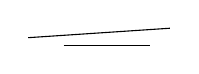
\begin{tikzpicture}
\draw (0,0)--(1.8,.12);
\draw (.45,-.10)--(1.55,-.10);
\end{tikzpicture}}

Nous nous proposons maintenant de relever $G_0$ \deleted{l'action} en un groupe de BT $G$ sur $A$, avec action de $A$ sur $G$, de telle façon que l'action \inserted{can.} de $A$ sur $t_G$ (qui est un $A$-module inversible) soit l'action évidente. D'après Lubin Tate,
\mspage{43}
\scanpage{45}
\mspage{44}
\mspage{78}
\margin{n°382}
\[
P_x^k:C_x^r(X)\longrightarrow P_x^k(X)
\]
soit un homomorphisme ; on a les formules :
\[
P_x^k(f)+P_x^k(g)=P_x^k(f+g),\quad
\lambda.P_x^k(f)=P_x^k(\lambda.f),\quad
P_x^k(f).P_x^k(g)=P_x^k(f.g),
\]
pour $f,g\in C_x^r(X)$, $\lambda\in K$.

7.1.3. Soit de plus h un morphisme dans une variété Z de classe $C^r$ d'un voisinage de y. Alors $j_x^k(h\circ f)$ ne dépend que de $j_x^k(f)$ et de $j_y^k(h)$ et on l'appelle le \uline{produit} (ou le \uline{composé}) de $j_x^k(f)$ et $j_y^k(h)$ ; le composé $v\circ u$ de deux jets u et v est donc défini si le but de u coïncide avec la source de v ; ce produit est associatif. Un jet u d'ordre k de X dans Y est \uline{inversible} s'il existe un jet $v\in J^k(Y,X)$ tel que $v\circ u$ et $u\circ v$ soient définis et égaux aux jets des applications identiques $1_X$ et $1_Y$. Si $k=0$, tout jet est inversible ; si $k\geq1$, un jet u est inversible si et seulement si c'est la partie principale d'ordre k d'un isomorphisme local de X dans Y ; dans ce cas, tout morphisme f tel que $j_x^k(f)=u$ est un isomorphisme local en x. Un jet d'ordre k inversible de X dans $K^p$ (resp. de source x) est appelé un \uline{repère d'ordre k} de X (resp. de source x). L'ensemble de ces repères est noté $R^k(X)$ (resp. $R_x^k(X)$). Si U et V sont des ouverts de X et Y, on a des inclusions canoniques
\[
J^k(U,V)\subset J^k(X,Y)\qquad\text{et}\qquad R^k(U)\subset R^k(X).
\]

7.1.4. Si $k'\leq k$, le jet $j_x^{k'}(f)$ d'ordre k' d'un germe de morphisme f ne dépend que de $j_x^k(f)$ et est inversible si $j_x^k(f)$ l'est. En faisant correspondre $j_x^{k'}(f)$ à $j_x^k(f)$, on définit des applications canoniques surjectives
\[
J_x^k(X,Y)_y\longrightarrow J_x^{k'}(X,Y)_y,\qquad
R_x^k(X)\longrightarrow R_x^{k'}(X)
\]
et $P_x^k(X)\longrightarrow P_x^{k'}(X)$ ; la dernière est un homomorphisme d'algèbres.

7.1.5. Soit $f=(f^1,\ldots,f^q)$ une application de classe $C^r$ d'un ouvert U de $K^p$ dans l'espace $K^q$. Si $x\in U$, le jet $j_x^k(f)$ de f est complètement déterminé par les coordonnées de sa source x et par les valeurs en x des fonctions $\Delta^\alpha f^i$, avec
\scanpage{46}
un tel relèvement existe et est unique (à isom \inserted{\unsure{non unique}} près). \deleted{\unsure{Et}} Pour simplifier et pouvoir appliquer la théorie des déformations, on va supposer que $\pi A$ est \unsure{stable|stble} par puissances divisées. Donc relever $G_0$ en un groupe de B.T $G$ sur $A$ (pour le moment sans nous préoccuper de l'action de $A$) revient à remonter la filtration de
\[
M\otimes_W k=M_A\otimes_A k
\]
en une filtration de $M_A$ (sur $A$).

\margin{$\Omega\qquad M=\Omega\otimes_{\mathbb Z_p}W\qquad M_A=\Omega\otimes_{\mathbb Z_p}A$
\diagram{\begin{tikzcd}
A\arrow[r,no head]\arrow[d,no head]&A\otimes_{\mathbb Z_p}W\arrow[r,no head]\arrow[d,no head]&A\otimes_{\mathbb Z_p}A\arrow[d,no head]\\
\mathbb Z_p\arrow[r,no head]&W\arrow[r,no head]&A
\end{tikzcd}}}

La compatibilité à l'action de $A$ signifie que c'est une filtration de $A\otimes_{\mathbb Z_p}A$-modules, i.e. un sous-\inserted{$A\otimes_{\mathbb Z_p}A$-}module \inserted{de rang $1$ sur $1\otimes A$} \deleted{de rang $1$} de $\Omega\otimes_{\mathbb Z_p}A$, (\unsure{le dernier sera} \deleted{\unsure{donc}} d'ailleurs can. isom. à $\omega_G$
\diagram{\begin{tikzcd}
0\arrow[r,no head]&\omega_G\arrow[r]&\Omega\otimes_{\mathbb Z_p}A\arrow[r]&t_{G^*}\arrow[r]&0
\end{tikzcd}}
ou, par transposition
\[
\unsure{(**)}
\]
\diagram{\begin{tikzcd}
0\arrow[r,no head]&\omega_{G^*}\arrow[r,no head]&\Omega^{\vee}\otimes_{\mathbb Z_p}A\arrow[r,"{\deleted{\unsure{\rho}}\varphi}"]&t_G\arrow[r]&0\\
&&A\otimes_{\mathbb Z_p}A\arrow[r,no head,"\rho_0"]&A
\end{tikzcd}}
L'hypothèse que l'action de $A$ \inserted{sur $t_G$} (via action sur $G$) est l'action de $A$-module naturelle, signifie que \deleted{\unsure{la structure}} \inserted{la structure de $A\otimes_{\mathbb Z_p}A$-module sur $t_G$ (ou $G$)} \deleted{\unsure{avec $A$-hom $\rho_0$ sur}} provient de la structure de $A$-module \deleted{triviale} évidente par \unsure{restriction} des scalaires à l'aide de
\[
\rho_0:A\otimes_{\mathbb Z_p}A\mathrel{\text{---}}A\qquad\rho_0(\lambda\otimes\mu)=\lambda\mu
\]
\mspage{45}
\scanpage{47}
\mspage{46}
\mspage{77}
\margin{n°382}

\S\ 7. \uuline{Jets. Opérateurs différentiels}.

A partir de maintenant, on adopte la convention suivante : si k est un entier, et si r désigne l'un des deux symboles $\infty$ et $\omega$, on pose $r-k=r$. Ainsi les dérivées d'ordre k d'une fonction de classe $C^r$ dans un ouvert de $K^n$ sont de classe $C^{r-k}$ dans cet ouvert, que r soit fini ou non.

7.1 -- \uline{Jets d'applications}.

7.1.1. Soient X et Y deux variétés de classe $C^r$, et soient $x\in X$, $y\in Y$ ; soient f et g deux morphismes d'un voisinage de x à valeurs dans Y, tels que $f(x)=g(x)=y$ ; soit k un entier positif $\leq r$, ou éventuellement le symbole $\infty$ si $r\geq\infty$. On dit que f et g ont un \uline{contact d'ordre} $\geq k$ \uline{en} x s'il existe une carte $(U,\varphi,p)$ de X en x et une carte $(V,\psi,q)$ de Y en y telles que $\psi\circ f\circ\varphi^{-1}$ et $\psi\circ g\circ\varphi^{-1}$ aient un contact d'ordre $\geq k$ au point $\varphi(x)\in K^p$ (cf. n° 1.1.1, 2.5.4). Cette propriété est alors vérifiée quel que soit le choix des cartes $(U,\varphi,p)$ et $(V,\psi,q)$ et définit une relation d'équivalence entre germes de morphismes. Une classe d'équivalence pour cette relation est appelée un \uline{jet d'ordre} k \uline{de morphisme} de X \uline{dans} Y, \uline{de source} x et \uline{de but} y ; la classe du morphisme f est notée $j_x^k(f)$ et se nomme le \uline{jet d'ordre} k de f en x, ou \uline{la partie principale d'ordre} k \uline{de} f en x. L'ensemble des jets d'ordre k de X dans Y (resp. de source x, resp. de but y) est noté $J^k(X,Y)$ (resp. $J_x^k(X,Y)$, resp. $J^k(X,Y)_y$), et l'on pose :
\[
J_x^k(X,Y)_y=J_x^k(X,Y)\cap J^k(X,Y)_y.
\]

7.1.2. Si $Y=K$, $J^k(X,Y)$ est l'ensemble des parties principales d'ordre k de fonctions morphiques sur X. On écrira en général $P^k(X)$, $P_x^k(X)$ et $P_x^k(f)$ pour $J^k(X,K)$, $J_x^k(X,K)$ et $j_x^k(f)$.

Soit $C_x^r(X)$ l'ensemble des germes en x de fonctions morphiques sur un voisinage de x ; c'est une K-algèbre. Il existe sur $P_x^k(X)$ une structure de K-algèbre et une seule telle que l'application
\scanpage{48}
Cela, plus le fait que $t_G$ et $\Omega^{\vee}\otimes_{\mathbb Z_p}A$ sont de rang $1$ sur $A$ resp. $A\otimes_{\mathbb Z_p}A$, et que $\unsure{\rho|\varphi}$ est surjectif, prouve que $t_G$ \uline{est déduit de} $\Omega^{\vee}\otimes_{\mathbb Z_p}A$ par le changt. de base
\diagram{\begin{tikzcd}A\otimes_{\mathbb Z_p}A\arrow[r,no head,"\rho_0"]&A\end{tikzcd}}
donc \deleted{\unsure{par suite}} (comme $\Omega^{\vee}\otimes_{\mathbb Z_p}A$ est déduit de $\Omega^{\vee}$ par $A\xrightarrow{\lambda\longrightarrow\lambda\otimes1}A\otimes_{\mathbb Z_p}A$) \unsure{on} obtient un isom can.
\[
t_G\simeq\Omega^{\vee}\qquad\text{i.e.}\qquad\omega_G\simeq\Omega
\]
et la suite exacte $(**)$ est la suite exacte canonique évidente, \inserted{d'où $(*)$ par dualité.} Comme cette filtration étend celle de $M_A\otimes_A k$, on a retrouvé ici le th. d'existence et d'unicité de Lubin-Tate, (sous une forme moins forte d'ailleurs en ce qui concerne l'unicité, et sous l'hyp. complémentaire que $\exists$ puiss. div. sur $\pi A$.

Si on abandonne cette dernière hypothèse, et qu'on utilise la classification des déformations à isogénie près, on trouve de $\unsure{=}$ qu'on a une suite exacte canonique
\diagram{\begin{tikzcd}
0\arrow[r,no head]&\omega_G\otimes_A K\arrow[r,no head]&M_K\arrow[r]\arrow[d,equal]&t_{G^*}\otimes_{\unsure{A}}K\arrow[r,no head]&0\\
&&\Omega\otimes_{\mathbb Z_p}K
\end{tikzcd}}
ou encore
\diagram{\begin{tikzcd}
0\arrow[r,no head]&\omega_{G^*}\otimes_A K\arrow[r,no head]&M_K^{\vee}\arrow[r]\arrow[d,equal]&t_G\otimes_A K\arrow[r]&0\\
&&\Omega^{\vee}\otimes_{\mathbb Z_p}K
\end{tikzcd}}
et on trouve encore que
\[
t_G\otimes_A K\simeq M_K^{\unsure{\vee}}\otimes_{\unsure{\Omega^{\vee}\otimes_{\mathbb Z_p}K}}(K\otimes K,\rho_0)\simeq\Omega^{\vee}\otimes_A K
\]
\mspage{47}
\scanpage{49}
\mspage{76}
\margin{n°382}
\[
\begin{aligned}
(f\omega)\wedge\omega'&=f.(\omega\wedge\omega')=\omega\wedge f\omega',\\
i(fs)\omega&=f.i(s)\omega=i(s)(f\omega),\quad\text{etc.}
\end{aligned}
\]
6.8.10. On définit de même la \uline{puissance symétrique} k-\uline{ième} $S^k(E)$ d'un espace fibré vectoriel E ; ses fibres sont égales aux puissances symétriques k-ièmes des fibres de E. On laisse au lecteur le soin de formuler, pour les puissances symétriques des résultats analogues à ceux énoncés ci-dessus pour les puissances extérieures.

6.9 -- \uline{Changement de structure}.

6.9.1. Soit E un espace fibré vectoriel de classe $C^r$ ; c'est aussi un espace fibré vectoriel de classe $C^{r'}$ pour tout $r'\leq r$, ainsi qu'un espace fibré vectoriel au sens topologique ; de même, s'il est analytique sur une extension de K, il l'est aussi sur K.

6.9.2. Les changements de structure définis au n° 6.9.1 sont compatibles avec la formation des images réciproques, ainsi qu'avec le \qquad procédé de construction du n° 6.6.
\begin{center}-:-:-:-\end{center}
\mspage{48}
\scanpage{50}
ce qui redonne la filtration de $M_K^{\vee}$ (ou de façon équivalente, de $M_K$) en termes de $\unsure{\ell|k}$.
Cela donne un th. d'unicité à isogénie près (mais pas d'existence ni d'unicité à \uline{isom} près, pour lesquels il faut ici se reporter à Lubin-Tate). Notons que $t_G$ et $\Omega^{\vee}$ s'identifient à un sous réseau de rang $1$ du $=$ vectoriel de dim $1$ sur $K$, donc (utilisant le choix de $\pi\in A$) ils sont can. isomorphes, \deleted{\unsure{isom. de}} par \deleted{\unsure{un}} $x\longmapsto\pi^{-\alpha}x$ ($\alpha\in\mathbb Z$ \unsure{unique}),
\[
t_G=\pi^{\deleted{\unsure{+}}-\alpha}\Omega^{\vee}\qquad\text{i.e.}\qquad\Omega=\pi^\alpha\omega_G,
\]
\deleted{On peut} où $\alpha\in\mathbb Z$ est bien déterminé (pour $A$ et $\pi$, et $=$ par $A$ tout seul, comme on voit \unsure{facilemt}...).

On a aussi
\[
D^*(G)_K\unsure{\sim}\simeq M_K\simeq\Omega\otimes_{\mathbb Z_p}K
\]
de sorte que $D^*(G)$ et $M$ s'identifient à des sous-réseaux du $=$ vectoriel sur $K$. On peut se demander si ces sous-réseaux sont les mêmes (comme dans le cas où $\exists$ puiss. div. sur $\pi A$), ce qui impliquerait évidemment $\unsure{\alpha'|\alpha}=0$.
Cela ne dépend pas du choix de $\pi$, mais seult de $A$

.....-
\mspage{49}
\scanpage{51}
\mspage{50}
\mspage{73}
\margin{n°382}
s'identifie à $\mathrm{Hom}^L(\bigotimes_{i=1}^{i=n}E_i,E)$, cf. n° 6.7.5. Soit U un ouvert de B, et soient $s_i\in S_{E_i}(U)$, $\varphi\in S_F(U)$ ; alors $\otimes s_i$ est une section $\bigotimes_{i=1}^{i=n}E_i$, et comme $\varphi$ s'identifie à un morphisme de $\bigotimes_{i=1}^{i=n}E_i$ dans E, $\varphi$ transforme $\otimes s_i$ en une section de E ; on la note $\langle\varphi,s_1\otimes\cdots\otimes s_n\rangle$, ou encore $\varphi(s_1,\ldots,s_n)$. C'est une fonction $C_L(U)$-multilinéaire de $\varphi$ et des $s_i$.

Inversement, supposons donné, pour tout ouvert U de B, une \uline{application} $C_L(U)$-\uline{multilinéaire} $\varphi_U$ \uline{de} $S_{E_1}(U)\times\cdots\times S_{E_n}(U)$ \uline{dans} $S_E(U)$, le système $(\varphi_U)$ \uline{commutant aux homomorphismes de restriction} (cf. n° 6.2.3. pour le cas $n=1$). Il existe alors une section $\varphi$ de F sur B et une seule qui correspond aux $\varphi_U$.

Lorsque tous les $E_i$ sont égaux, et que l'on remplace F par $F'=\bigwedge^n E_1^*\otimes E=\mathrm{Hom}^L(\bigwedge^n E_1,E)$ (cf. n° 6.8.7), on a un résultat analogue, les applications $\varphi_U$ étant cette fois des applications multilinéaires \uline{alternées}.

6.8 -- \uline{Espaces tensoriels}, \uline{puissances extérieures}, \uline{puissances symétriques}.

Les espaces fibrés vectoriels considérés dans ce numéro sont relatifs à un corps L et à une base B fixés ; on suppose que L est \uline{commutatif}.

6.8.1. Soit E un espace fibré vectoriel, et soient I et J deux ensembles finis disjoints. Le \uline{fibré tensoriel} $T_J^I(E)$ est défini comme le produit tensoriel $\bigotimes_{\alpha\in I\cup J}E_\alpha$, où $E_\alpha=E$ si $\alpha\in I$, et $E_\alpha=E^*$ si $\alpha\in J$, $E^*$ désignant le dual de E (cf. \uline{Alg.}, chap. III, 3ème édition, \S\ \qquad, n°\qquad). La fibre $T_J^I(E)_b$ de ce fibré en un point b est égale à l'espace tensoriel $T_J^I(E_b)$ défini en \uline{Alg.}, \uline{loc.} \uline{cit.}. Lorsque $I=\{1,\ldots,p\}$ et $J=\{p+1,\ldots,p+q\}$, on écrit $T_q^p(E)$ au lieu de $T_J^I(E)$ ; on a
\[
T_q^p(E)=(\otimes^p E)\otimes(\otimes^q E^*).
\]
La donnée d'un \uline{ordre total} sur I et sur J définit un isomorphisme canonique de $T_J^I(E)$ sur $T_q^p(E)$.
\scanpage{52}
Nous allons examiner \deleted{d'ailleurs} ce que donne le théor. de Tate, pour le groupe de Lubin Tate $G_{\unsure{\varepsilon}}$.
Notons que, si $K_\pi\subset\overline K$ est l'extension \inserted{abélienne} de groupe $A^*$ définie par $G$ (via $\mathrm{Gal}(\overline K/K)\xrightarrow{\chi_\pi}A^*$), alors \deleted{\unsure{un}} $T_p(G)(\overline K)$ est un module inversible sur $A$, et les bases de celui-ci sont permutées de façon simplement transitive par $\mathrm{Gal}(K_\pi/K)$. Donc, il y a un choix privilégié (à isom \uline{unique} près) d'une extension algébrique $K_\pi$ de $K$ (indépendant du choix d'une clôture $\overline K$ !) avec un générateur
\[
e\in T_p(G)^*(K_\pi)
\]
[en fait, $\mathrm{Spec}\,K_\pi$ représente le foncteur $T_p(G)^*=\varprojlim G(\nu)^*$, où le $*$ désigne les générateurs \deleted{\unsure{comme}} $A$-modulaires]. Nous supposons fixé $K_\pi$ de cette façon, et choisissons pour $\overline K$ une surextension de $K_\pi$. Donc le choix de $e$ donne un isom de $A$-modules
\[
\overbrace{T_p(G)(K_\pi)}^{T_p}\simeq A,\qquad\lambda\longmapsto\lambda e.
\]
\margin{\diagram{\begin{tikzcd}
T_p\arrow[d,equal]&T_p\otimes A\arrow[d,equal]&T_p\otimes C\arrow[d,equal]\\
A\arrow[r,no head]\arrow[d,no head]&A\otimes_{\mathbb Z_p}A\arrow[r,no head]\arrow[d,no head]&A\otimes_{\mathbb Z_p}C\arrow[d,no head]\\
\mathbb Z_p\arrow[r,no head]&A\arrow[r,no head]&C
\end{tikzcd}}}
On regarde sur $T_p(\unsure{G})\otimes_A C$ d'une part l'action de $A$ provenant de l'action de $A$ sur $G$, (``action à opérateurs'') d'autre part l'action provenant de la structure de $C$-vectoriel. Enfin, on a l'action de $\pi=\mathrm{Gal}(\overline K/K)$, qui commute à l'action (opér.) de $A$. Supposons $K/\mathbb Q_p$ galoisien pour simplifier.
\mspage{51}
\scanpage{53}
\mspage{43}
\margin{n°382}

4.13 -- \uline{Affaiblissement de structure}.

Dans tout ce numéro, on suppose que $K=\uuline{R}$ ; on note I l'ensemble $\{1,2,\ldots,n,\ldots;\infty;\omega\}$. Nous ordonnerons I par la relation d'ordre usuelle sur les entiers, étendue à $\infty$ et à $\omega$ au moyen des formules
\[
n<\infty<\omega.
\]

4.13.1. Soient $r,s\in I$, avec $r\leq s$, et soit X une variété de classe $C^s$. Il existe sur l'espace topologique X une structure de variété de classe $C^r$ et une seule telle que toute carte de X pour la structure donnée soit une carte de X pour cette nouvelle structure. Soit $X_r$ la variété de classe $C^r$ ainsi définie. On dit qu'elle se déduit de X par \uline{affaiblissement} de la structure de variété de X ; ou encore que sa structure de variété est \uline{sous-jacente} à celle de X. La notion d'affaiblissement est transitive : si $r'\leq r$, on a $X_{r'}=(X_r)_{r'}$ ; elle commute aux produits : si Y est de classe $C^s$, on a $(X\times Y)_r=X_r\times Y_r$ ; on a un résultat analogue pour $X\times_S Y$ sous les hypothèses du n° 4.11.3.

Soit $a\in X$ et soit c une carte de X en a ; c'est aussi une carte de $X_r$ en a. On en déduit (cf. n° 4.5.1) des isomorphismes
\[
\vartheta_c:K^n\longrightarrow T_a(X),\qquad
\vartheta'_c:K^n\longrightarrow T_a(X_r),\qquad n=\dim_x(X),
\]
d'où un isomorphisme $\vartheta'_c\circ\vartheta_c^{-1}:T_a(X)\longrightarrow T_a(X_r)$. Cet isomorphisme est indépendant du choix de c ; il permet \uline{d'identifier les espaces tangents} à X et à $X_r$ en a.

4.13.2. Soit X (resp. X') une variété de classe $C^s$ (resp. $C^{s'}$), et soit $r\in I$, $r\leq\operatorname{Inf}(s,s')$. Une application $f:X\longrightarrow X'$ est dite \uline{de classe} $C^r$ si c'est un morphisme de $X_r$ dans $X'_r$ ; une telle application est de classe $C^{r'}$ pour tout $r'\leq r$. De plus, l'application linéaire tangente à $f:X_r\longrightarrow X'_r$ en un point $a\in X$ coïncide avec l'application linéaire tangente à f considérée comme morphisme de $X_{r'}$ dans $X'_{r'}$. Pour que $f:X_r\longrightarrow X'_r$ soit une submersion (resp. une immersion, une subimmersion), il faut et il suffit que $f:X_{r'}\longrightarrow X'_{r'}$ en soit une ; on dira alors plus simplement que f est une submersion (resp. une immersion, resp. une
\mspage{52}
\scanpage{54}
Alors comme module sur $A_C$, \deleted{$T_p\otimes C$ s'identifie} \inserted{on a un isom} canonique
\[
\unsure{(*)}\qquad\boxed{T_p\otimes_{\mathbb Z_p}C\simeq\prod_\sigma C_\sigma},
\]
où $C_\sigma=C$, comme $C$-vectoriel, l'opération de $A$ dessus se faisant via $\sigma:A\mathrel{\text{---}}C$, où
\[
\sigma\in\operatorname{Hom}_{\mathbb Q_p}(K,C)\xleftarrow{\sim}\operatorname{Aut}_{\mathbb Q_p}(K)\simeq\operatorname{Aut}_{\mathbb Z_p}(A)\simeq\operatorname{Hom}_{\mathbb Z_p}(A,C).
\]
\margin{$*$}
Cette décomposition est compatible avec l'action de $\pi$, de façon précise, $\pi$ opère sur le facteur $C_\sigma$ par $\rho_\sigma(g)$ ($g\in\pi$) donné par
\[
x\in C_\sigma\Longrightarrow\rho_\sigma(g)x=\sigma(\chi_\pi(g))x
\]
Comparons cette décomposition avec celle donnée par le théor. de Tate
\diagram{\(\left\{\begin{gathered}
\begin{tikzcd}
0\arrow[r]&\mathfrak g\otimes C(1)\arrow[r]&T_p\otimes C\arrow[r]\arrow[l,dashed,bend left=35]&\check{\mathfrak g}^{*}\otimes C\arrow[r]\arrow[l,dashed,bend left=35]&0
\end{tikzcd}\\[2em]
T_p\otimes C)\simeq\mathfrak g\otimes_A C(1)+\check{\mathfrak g}^{*}\otimes_A C
\end{gathered}\right.\quad(**)\)}
Notons que ce dernier isom. est fonctoriel, donc commute à l'action de $A$ sur les deux mbres. Or \inserted{on a vu que} l'action de $A$ sur $\mathfrak g$ est l'action régulière, l'action de $A$ sur $\check{\mathfrak g}^{*}\otimes C$ se fait suivant les hom $A\longrightarrow C$ pour $\sigma\ne1$. Donc la décomposition $(**)$ de $T_p\otimes C$ est celle déduite de la décomposition $(*)$ en \deleted{\unsure{y groupant}} l'écrivant
\[
T_p\otimes C\simeq C_1\oplus\prod_{\sigma\ne1}C_\sigma.
\]
\deleted{Il faut} En tant qu'isomorphisme can., \unsure{est|elle}
\mspage{53}
\scanpage{55}
\mspage{42}
\margin{n°382}
\[
\begin{aligned}
s(tx)&=(st)x&&\text{si}\quad s,t\in G,\ x\in X\\
ex&=x&&\text{si}\quad x\in X\quad(e\text{ étant l'élément neutre de }G).
\end{aligned}
\]
On dit aussi que G \uline{opère à gauche} sur X ; on définit de même les lois d'opération à droite.

Soit $x\in X$, et soit $G_x$ son stabilisateur dans G. Supposons que l'application $g\longrightarrow g.x$ soit une \uline{subimmersion} (hypothèse automatiquement vérifiée si la caractéristique de K est 0). Alors $G_x$ est une sous-variété de groupe, et l'application de $G/G_x$ dans X obtenue par passage au quotient à partir de $g\longrightarrow g.x$ est une immersion. Si en outre l'orbite $Gx$ de x est localement fermée, et si la topologie de G admet une base dénombrable, $Gx$ est une sous-variété de X, et l'application $G/G_x\longrightarrow Gx$ est un isomorphisme.

4.12.6. Soit $\varpi:G\longrightarrow S$ une submersion, G et S étant deux variétés. Pour tout $s\in S$, soit $G_s=\varpi^{-1}(s)$. Supposons que chacun des $G_s$ soit muni d'une structure de groupe, vérifiant les deux conditions suivantes :

(i) L'application $e:S\longrightarrow G$ qui applique $s\in G$ en l'élément neutre $e(s)$ de $G_s$ est un morphisme.

(ii) L'application de $G\times_S G$ dans G définie par $(x,y)\longrightarrow x^{-1}y$ est un morphisme.

On dit alors que G est un \uline{groupe au-dessus de} S, ou encore un S-\uline{groupe}. Pour tout $s\in S$, $G_s$ est une sous-variété de G, et sa structure de variété est compatible avec sa structure de groupe.

Si G est un S-groupe, l'application $x\longrightarrow x^{-1}$ est un morphisme de G dans lui-même ; l'application $(x,y)\longrightarrow xy$ est un morphisme de $G\times_S G$ dans G.

4.12.7. Soit $\varpi:G\longrightarrow S$ un S-groupe, et soit $f:T\longrightarrow S$ un morphisme. Soit $G(T)$ l'ensemble des morphismes $\varphi:T\longrightarrow G$ tels que $\varpi\circ\varphi=f$. Si $\varphi,\psi\in G(T)$, soit $\varphi.\psi$ le composé de $(\varphi,\psi)_S:T\longrightarrow G\times_S G$ avec l'application $(x,y)\longrightarrow xy$ de $G\times_S G$ dans G ; on a $\varphi.\psi\in G(T)$ et la loi de composition ainsi définie fait de $G(T)$ un groupe d'élément neutre $e\circ f$.
\mspage{54}
\scanpage{56}
tenant compte des isom \inserted{can.} obtenus plus haut (de $A\otimes C$-modules)
\[
\mathfrak g\otimes_A C\simeq C_1,\qquad\check{\mathfrak g}^{*}\otimes_A C\simeq\prod_{\sigma\ne1}C_\sigma,
\]
\deleted{Il faut donc définir} \inserted{le théor. de Tate donne} des isom de $A\otimes_{\mathbb Z_p}C$-modules
\[
C_\sigma\longrightarrow C_\sigma,\quad\text{i.e.}\quad\lambda\longmapsto\lambda x_\sigma\quad(x_\sigma\in C)
\]
qui commutent à l'action de $\pi$ opérant sur la source par $*$, et sur le but par \deleted{\unsure{$g$}} $x\longmapsto g(x)$ si $\sigma\ne1$, par $x\longrightarrow\tau(\unsure{x|g})g(x)$ si $\sigma=1$ ($\tau$ étant la \unsure{contorsion} de Tate) Cela revient aux conditions
\[
\boxed{\left\{\begin{aligned}
g(x_\sigma)&=\sigma(\chi_\pi(g))x_\sigma&&\text{si }\sigma\ne1\\
g(x_1)&=\tau(g)^{-1}\chi_\pi(g)x_1&&\text{si }\sigma=1
\end{aligned}\right.\quad\Biggr\}\ \text{si }g\in\underset{\substack{\Vert\\\mathrm{Gal}(\overline K/K)}}{\pi}}
\]
\uline{NB} A priori, les $x_\sigma$ sont déterminés par la condition écrite modulo multiplication par un élém de $A^*\subset K^*\subset C^*$. Mais \unsure{le} (\unsure{sous participation seule|sans particularisation} du choix de $\overline K$) le choix de l'un de ces $x_\sigma$ \inserted{(disons, de $x_1$)} détermine canoniquement, par le théor. de Tate, tous les autres. \deleted{\unsure{De cette façon}}

Il n'existe pas de $x'_1\in C^*$ tel qu'on ait
\[
g(x'_1)=\chi_\pi(g)x'_1\qquad\text{pour }g\in\pi\ (\text{ni }=\text{ pour }J\subset\text{Inertie de }\pi)
\]
car faisant le produit de $x'_1$ et des $x_\sigma$ ($\sigma\ne1$), on trouverait $x\in C^*$ tel que
\[
g(x)=\underbrace{N_{A/\mathbb Z_p}(\chi_\pi(g))}_{=\tau(g)\text{ si }g\in\text{Inertie}}x,\qquad\text{impossible.}
\]
\mspage{55}
\scanpage{57}
\mspage{40}
\margin{n°382}
est formé des couples $(h,k)\in T_x(X)\times T_y(Y)$ tels que $T_x(f).h=T_y(g).k$.

Le morphisme $g':X\times_S Y\longrightarrow X$ est parfois appelé \uline{l'image réciproque} du morphisme $g:Y\longrightarrow S$ par f ; par abus de langage, on dit aussi que $X\times_S Y$ est \uline{l'image réciproque de} Y \uline{par} f. Si g est une submersion (resp. une immersion), il en est de même de g'. Si X est une sous-variété de S, et si f est l'injection canonique de X dans S, le couple $(f,g)$ est transversal si et seulement si g est transversal à X (cf. n° 4.11.1) ; de plus, f' induit un isomorphisme de $X\times_S Y$ sur la sous-variété $g^{-1}(X)$ de Y (ce qui justifie, dans ce cas, le terme d' ``image réciproque'' appliqué à $X\times_S Y$). En particulier, $S\times_S Y$ s'identifie à Y.

4.11.4. Soit $f:X\longrightarrow S$, $g:Y\longrightarrow S$ un couple transversal de morphismes. Soit T une variété, et soient $u:T\longrightarrow X$, $v:T\longrightarrow Y$ des morphismes tels que $f\circ u=g\circ v$. Il existe alors un morphisme $j:T\longrightarrow X\times_S Y$ et un seul tel que $u=g'\circ j$, $v=f'\circ j$, les notations étant celles du n° précédent. Le morphisme j se note $(f,g)_S$.

4.12 -- \uline{Variétés de groupes}.

4.12.1. Soit G un groupe. Une structure de variété sur G est dite \uline{compatible} avec la structure de groupe de G si l'application $(x,y)\longrightarrow xy$ de $G\times G$ dans G est un morphisme, ainsi que l'application $x\longrightarrow x^{-1}$ de G dans lui-même. Muni de ces deux structures, G est appelé une \uline{variété de groupe} (``de classe $C^r$'' si l'on veut préciser) ; pour $r=\omega$ (resp. $r\ne\omega$), on dit aussi ``groupe analytique'' (resp. ``groupe différentiable''). Toute variété de groupe est pure. On appelle \uline{morphisme de variétés de groupe} (ou simplement \uline{morphisme}) toute application d'une variété de groupe dans une autre qui est à la fois une \uline{représentation} de groupes et un \uline{morphisme} de variétés.

Si G est une variété de groupe, la structure topologique sous-jacente à la structure de variété de G en fait un \uline{groupe topologique métrisable et complet} ; il est localement compact si K est localement compact.
\mspage{56}
\scanpage{58}
\mspage{57}
\figure{\begin{tikzpicture}[x=.008cm,y=-.008cm,line width=.18pt,every node/.style={font=\tiny,inner sep=1pt}]
\node at (141,137) {$\dfrac{\unsure{n|4}}{17}$};
\node at (644,43) {$\nu$};
\draw (594,68)--(692,58);
\node at (258,126) {$n=1,2,3$};
\draw (374,134)--(414,138)--(565,76);
\draw (374,134)--(565,72);
\draw (384,135)--(450,137);
\node at (647,106) {$1$};
\node at (249,182) {$n=4$};
\draw (384,195)--(443,187)--(556,137);
\draw (384,195)--(454,193)--(552,143);
\draw (386,196)--(548,144);
\fill (443,187) circle[radius=1.8];
\node at (642,177) {$2$};
\node at (254,250) {$n=5$};
\draw (384,264)--(448,254)--(488,241)--(553,192)--(553,260)--cycle;
\draw (386,260)--(451,258)--(488,245)--(550,197);
\draw (389,263)--(444,267)--(486,263);
\fill (448,254) circle[radius=2];
\fill (488,241) circle[radius=2];
\fill (553,249) circle[radius=1.6];
\node at (644,231) {$3$};
\node at (258,319) {$n=6$};
\draw (396,331)--(433,333)--(600,268)--cycle;
\draw (399,330)--(458,312)--(599,269);
\draw (407,331)--(598,272);
\node at (651,298) {$1$};
\node[align=left] at (301,406) {$n=7,8,9,10,11$\\$12,13$};
\draw (399,395)--(467,382)--(632,313);
\draw (399,395)--(458,403)--(632,313);
\draw (459,399)--(626,319);
\fill (467,382) circle[radius=1.8];
\node at (640,374) {$2$};
\node at (273,500) {$n=14$};
\draw (426,490)--(467,490)--(520,464)--(567,419);
\node at (641,460) {$3$};
\node at (279,562) {$n=\unsure{15,16}$};
\draw (431,554)--(473,548)--(556,505);
\node at (634,520) {$2$};
\draw[very thin] (617,145)..controls (613,274) and (624,360)..(616,487);
\draw (306,1100)--(1438,1092)--(1438,960);
\draw (369,1030)--(1438,1022)--(1438,960);
\draw[very thin] (306,1032)--(1424,20);
\draw[very thin] (312,1030)--(1430,20);
\draw[very thin] (369,1030)--(431,965)--(494,903)--(557,839)--(620,775)--(682,711)--(745,651)--(807,586)--(869,520)--(1433,67);
\draw[very thin] (431,965)--(619,775)--(809,585)--(1057,324)--(1433,135);
\draw[very thin] (494,903)--(682,711)--(870,520)--(1060,383)--(1433,199);
\draw[very thin] (557,839)--(682,711)--(808,707)--(1120,454)--(1433,256);
\draw[very thin] (620,775)--(807,707)--(931,582)--(1184,454)--(1433,321);
\draw[very thin] (682,711)--(870,707)--(1058,583)--(1217,520)--(1433,387);
\draw[very thin] (745,651)--(868,648)--(994,584)--(1181,584)--(1433,448);
\draw[very thin] (1056,644)--(1246,580)--(1433,511);
\draw[very thin] (807,837)--(995,770)--(1182,671)--(1433,575);
\draw[very thin] (869,837)--(995,837)--(1176,744)--(1433,639);
\draw[very thin] (494,903)--(682,903)--(807,837)--(994,769)--(1433,700);
\draw[very thin] (431,965)--(620,965)--(807,903)--(1058,835)--(1433,766);
\draw[very thin] (369,1030)--(557,1030)--(806,964)--(1119,895)--(1433,832);
\draw[very thin] (431,1030)--(745,1030)--(994,965)--(1433,894);
\draw[very thin] (557,1030)--(994,1026)--(1433,960);
\draw (1367,116)--(1433,67);
\draw (1308,237)--(1433,135);
\draw (1306,292)--(1433,199);
\draw (1369,299)--(1433,256);
\draw (1308,393)--(1433,321);
\draw (1245,490)--(1433,387);
\draw (1307,515)--(1433,448);
\draw (1371,543)--(1433,511);
\draw (1371,602)--(1433,575);
\draw (1307,686)--(1433,639);
\draw (1307,742)--(1433,700);
\draw (1307,800)--(1433,766);
\draw (1307,854)--(1433,832);
\draw (1307,910)--(1433,894);
\foreach \x/\y in {369/1030,431/965,494/903,557/839,620/775,682/711,745/651,807/586,869/520,931/518,994/454,1057/324,1120/260,1183/194,807/707,870/707,995/583,1182/518,807/837,995/770,620/903,807/964,995/837,1433/67,1433/135,1433/199,1433/256,1433/321,1433/387,1433/448,1433/511,1433/575,1433/639,1433/700,1433/766,1433/832,1433/894,1438/960,1438/1022,369/1100}
 {\fill (\x,\y) circle[radius=1.5];}
\foreach \n/\x in {1/340,2/402,3/465,4/528,5/591,6/654,7/718,8/781,9/844,10/907,11/970,12/1033,13/1096,14/1159,15/1222,16/1285,17/1348,18/1411}
 {\node at (\x,1140) {$\n$};}
\foreach \n/\y in {1/995,2/930,3/870,4/806,5/738,6/676,7/613,8/550,9/487,10/421,11/357,12/292,13/229,14/167,15/102,16/45}
 {\node at (1474,\y) {$\n$};}
\node at (1680,44) {$\deleted{\unsure{m}}\,\unsure{n}$};
\node at (1593,109) {$\deleted{7}\ \dfrac{6}{9}>\dfrac{11}{17}$};
\node at (1631,167) {$\dfrac{2}{3}>\dfrac{11}{17}$};
\node at (1597,315) {$\dfrac{5}{12}>\dfrac{7}{17}$};
\node at (1632,389) {$\dfrac{1}{4}<\dfrac{\unsure{3}}{11}<\dfrac{2}{7}$};
\node at (1608,476) {$\dfrac{2}{7}<\dfrac{5}{17}$};
\node at (1621,641) {$\dfrac{4}{17}\unsure{<|>}\dfrac{1}{4}$};
\node at (1595,769) {$\dfrac{1}{9}<\dfrac{2}{17}$};
\node at (1598,871) {$\dfrac{1}{6}<\dfrac{3}{17}$};
\node at (929,716) {$253\unsure{>|\geq}\unsure{285|295}$};
\node at (874,750) {$2$};
\draw (888,751)..controls (878,760) and (880,769)..(878,775);
\node at (111,806) {$\dfrac{4}{13}>\dfrac{7}{23}$};
\node[rotate=-14] at (225,880) {$<\unsure{5/12}$};
\node at (137,955) {$3/10>\dfrac{7}{24}$};
\node at (117,1059) {$\deleted{\unsure{\dfrac{4}{5}}}\ \dfrac{2}{\unsure{3|7}}<\dfrac{7}{24}$};
\node at (100,1163) {$\dfrac{1}{3}>\dfrac{7}{23}$};
\node at (151,1217) {$\deleted{\unsure{\dfrac{1}{7}}}$};
\node at (125,1286) {$\dfrac{2}{7}\unsure{\ll|<}\dfrac{1}{3}$};
\node at (321,1275) {$7/9<\dfrac{7}{\unsure{0|8}}$};
\node at (521,1275) {$\dfrac{4}{5}<\dfrac{14}{17}$};
\node at (756,1204) {$\dfrac{11}{17}\unsure{>|<}\dfrac{15}{23}\ ;\quad 2/3>\dfrac{15}{23}$};
\draw (594,1155)--(594,1210)..controls (594,1248) and (603,1245)..(645,1245)--(925,1230);
\node at (748,1274) {$\dfrac{10}{14}<\dfrac{13}{18}$};
\node at (977,1270) {$\dfrac{13}{17}<\dfrac{10}{13}\ \deleted{\unsure{\dfrac{7}{8}|\dfrac{2}{8}}}$};
\node at (1146,1209) {$3/5<\dfrac{14}{23}$};
\node at (1247,1277) {$3/4<\dfrac{13}{17}$};
\node at (1486,1277) {$\dfrac{5}{7}\unsure{<|>}\dfrac{13}{18}$};
\node at (1595,1175) {$\dfrac{7}{10}<\dfrac{12}{17}$};
\end{tikzpicture}}
\scanpage{59}
\figure{\begin{tikzpicture}[x=.008cm,y=-.008cm,line width=.2pt,every node/.style={font=\small,inner sep=1pt}]
\draw (287,1029)--(1313,1016);
\draw (1311,1008)--(1313,1021);
\draw (303,966)--(305,1028);
\draw (305,1028)--(1302,132);
\draw (305,1028)--(429,960)--(1302,195);
\draw (305,1028)--(365,1028)--(1302,195);
\draw[very thin] (305,1028)--(553,834)--(618,772)--(679,708)--(742,644)--(804,579)--(1302,132);
\draw[very thin] (365,1028)--(553,840)--(742,665)--(926,516)--(1120,350)--(1302,195);
\draw[very thin] (369,1014)--(367,1023)--(365,1012);
\foreach \x/\y in {305/1028,365/1028,429/960,490/897,553/834,618/772,679/708,742/644,804/579,865/579,926/516,1302/132,1302/195}
 {\fill (\x,\y) circle[radius=1.5];}
\node at (1531,103) {$\dfrac{4}{5}<\dfrac{13}{15}$};
\node at (1544,218) {$\dfrac{12}{14}=\dfrac{6}{7}$};
\node at (1535,552) {$\dfrac{14}{16}=\dfrac{7}{8}<$};
\end{tikzpicture}}
\mspage{58}
\scanpage{60}
\figure{\begin{tikzpicture}[x=.008cm,y=-.008cm,line width=.2pt,every node/.style={font=\small,inner sep=1pt}]
\node at (1155,171) {$13/15<\dfrac{7}{8}$};
\node at (1129,323) {$\dfrac{3}{4}>\dfrac{11}{15}$};
\node at (1133,416) {$\dfrac{2}{3}<\dfrac{11}{16}$};
\node at (1129,526) {$\unsure{\dfrac{6}{11}}\unsure{\geq|\neq}\dfrac{1}{2}$};
\node at (485,441) {$\dfrac{12}{14}=\dfrac{6}{7}$};
\draw (47,1140)--(1057,1123);
\draw (47,1127)--(47,1140)--(175,1077)--(1048,305);
\draw (111,1140)--(175,1077)--(236,1014)--(300,949)--(361,885)--(609,692)--(670,629)--(1048,305);
\draw[very thin] (47,1140)--(300,918)--(609,657)--(1048,305);
\draw[very thin] (111,1140)--(361,914)--(670,638)--(1048,305);
\foreach \x/\y in {47/1140,111/1140,175/1077,236/1014,300/949,361/885,609/692,670/629,1048/305,1049/624,1053/811,1054/875}
 {\fill (\x,\y) circle[radius=1.7];}
\draw (43,1460)--(175,1395)--(239,1329)--(366,1265)--(427,1199)--(554,1124)--(615,1069)--(1053,748);
\draw (47,1461)--(1053,748);
\draw (111,1457)--(366,1265)--(1053,748);
\draw[very thin] (47,1461)--(237,1330)--(428,1199)--(739,977)--(1053,748);
\draw[very thin] (47,1461)--(428,1260)--(1053,937);
\draw[very thin] (111,1457)--(1053,937);
\draw (987,976)--(1053,937);
\draw[very thin] (47,1461)--(492,1260)--(1055,997);
\draw[very thin] (111,1457)--(1055,997);
\draw (927,1062)--(1055,997);
\draw[very thin] (47,1461)--(367,1386)--(556,1322)--(808,1254)--(1058,1189);
\draw (111,1457)--(1058,1189);
\draw[very thin] (47,1461)--(556,1384)--(1060,1316);
\draw[very thin] (111,1457)--(1060,1316);
\draw[very thin] (1053,748)--(1062,1455);
\foreach \x/\y in {47/1461,111/1457,175/1395,239/1329,305/1323,305/1388,366/1265,427/1199,492/1260,554/1124,554/1260,556/1322,615/1069,808/1254,1053/748,1053/937,1055/997,1058/1189,1060/1316}
 {\fill (\x,\y) circle[radius=1.5];}
\end{tikzpicture}}
\mspage{59}
\scanpage{61}
\deleted{\unsure{$G$}}

Groupe de galois d'une catégorie tannakienne \inserted{\unsure{graduée|gr. duée}} \inserted{($\mathbb Q_p$-linéaire)} $1/2$ simple $C$ munie d'un foncteur fibre à valeurs dans les \inserted{$F$-}cristaux \inserted{filtrés \unsure{gradués|gr. dués}} à isogénie près sur un anneau \deleted{local} \inserted{de} Val. discr. complet $V$ d'inégales car., à corps résiduel parfait $k$, corps des fractions $L$.

On a
\margin{\unsure{vect. Witt}}
\diagram{\[
\begin{array}{ccc}
W&\subset&V\\
\cap&&\cap\\
K&\subset&L
\end{array}
\]}

a) foncteur \inserted{fibre $\Phi$} vers les $F$-cristaux sur $k$ à isogénie près

$=$ certains couples $(E,F)$, où $E$ vectoriel de dim. finie sur $K$, $F$ endomorphisme $\sigma$-linéaire de $E$, tel qu'il existe un réseau invariant par $F$.

b) filtration de $\Phi\otimes_K L$.

\deleted{Le foncteur $\Phi$ \inserted{(en oubliant la $F$ structure)} \unsure{permet} d'identifier $C$ à la catégorie des repr. lin. sur $K$}

Le foncteur fondamental \inserted{(\unsure{convenable})} fournit un foncteur
\[
\unsure{T_p|V_p}:C\longrightarrow\operatorname{Mod}_f(\pi,\mathbb Q_p)
\]
où
\[
\pi=\operatorname{Gal}(\overline L/L)
\]
donc \uline{on a un foncteur fibre sur} $\mathbb Q_p$, correspondant à une représentation (à équiv. près) de $C$ comme
\[
C\simeq\operatorname{Rep}_{\mathbb Q_p}(G)
\]
$\boxed{G}$ étant un groupe pro-réductif sur $\mathbb Q_p$.
\mspage{60}
\scanpage{62}
\mspage{61}
\mspage{35}

\deleted{\unsure{et}} $S'\longrightarrow S$. Posons dans cet situation
\[
\psi(S,Z,Y,X)=\xi\eta\varphi(Z,Y),
\]
d'où $\psi$ est de nature locale et commute aux changements de base. Or si $(Z,X)$ est un couple lisse de codimension $c>1$, on peut, localement sur $X$, trouver un triple $(Z,Y,X)$ avec $0<\operatorname{codim}(Y,X)<c$. Tout revient donc à démontrer que la flèche $\psi(S,Z,Y,X)$ est indépendant de $Y$. En effet, cela démontrera l'unicité de \qquad pour codimension $c$, et l'existence résultera de descente.

Si $(Z,Y,X)$ est arbitraire tel que $\operatorname{codim}(Y,X)>1$, on peut, localement sur $X$, trouver un triple lisse $(Y,W,X)$ où la dodimension de $(W,X)$ est égal à 1. Par une chasse de diagramme de transitivité, que nous laissons au lecteur\unsure{\}|,} on se ramène donc à vérifier l'indépendance de $Y$ lorsque $(Y,X)$ est de codimension 1. Soient \deleted{\unsure{$(Z,Y_1,X)$ et $(Z,Y_0$}} $(Z,Y_0,X)$ et $(Z,Y_1,X)$ deux tels triples. Puisque le problème est local, nous pouvons supposer que $Y_0$ et $Y_1$ sont définis chacun par une équation dans $X$, disons $f_0=0$ resp. $f_1=0$.

Soit $\overline S=\uline{\operatorname{Spec}}O_S[t]$, $\overline X=X\times_S\overline S$, $\overline Z=Z\times_S\overline S$, et soit $\overline Y$ le sous-schéma de $\overline X$ défini par l'équation
\[
(f_1-f_0)t+f_0=0.
\]
Alors $\overline Y/\overline S$ est lisse en les points au dessus des
\scanpage{63}
Pour simplifier, on supposera que $C$ est de \unsure{t.f.} sur $\mathbb Q_p$. De plus, on a un hom
\diagram{\[\boxed{\begin{tikzcd}
\pi\arrow[r,"\alpha"]&G(\unsure{\mathbb Q_\ell|\mathbb Q_p})
\end{tikzcd}}\]}
Si le foncteur \deleted{\unsure{$\Phi$}} $T_p$ (ou, ce qui revient au même, \deleted{\unsure{pl.}} le foncteur $\Delta$) est pl. fidèle, dans cet cas seulement) $G$ est l'enveloppe algébrique de $\alpha$.

De plus, le composé
\diagram{\[
\begin{tikzcd}[column sep=small]
C\arrow[r,no head]&\operatorname{Mod}_f(\pi,\mathbb Q_p)\arrow[r,no head,"{\otimes_{\mathbb Q_p}C}"]&\operatorname{Mod}_f(\pi,C)\arrow[r,no head]&\operatorname{Mod}_f(C)
\end{tikzcd}
\]}
est un foncteur \uline{bigradué}, \deleted{\unsure{i.e. on a un}} (gradué par degré total, et par décomposition de Hodge)

donc on a
\diagram{\[\boxed{\begin{tikzcd}
Gm_C\arrow[r,shift left=.6ex,"i_1"]\arrow[r,shift right=.6ex,"i_2"']&G_C
\end{tikzcd}}\]}
avec
\[
\unsure{i'|i}(\lambda)=i_1(\lambda)i_2(\lambda)=i(\lambda):\quad Gm_C\longrightarrow G_C
\]
l'hom \uline{central} définissant la graduation de $C$.

De plus, on a un \deleted{hom} foncteur fibre \inserted{$T_{\mathrm{Hdg}}$} bigradué ``de Hodge'' sur $K$, donc défini par
\[
\left\{\begin{gathered}
\boxed{P,\ \text{torseur pour }G_L}\\
(\overline T_{\mathrm{Hdg}}=P\mathbin{\wedge}^{G_L}(T_p\otimes_{\mathbb Q_p}L)\ \deleted{\unsure{et}}
\end{gathered}\right.
\]
\deleted{et}
\diagram{\[
\left\{\begin{gathered}
\begin{tikzcd}
Gm_L\arrow[r,shift left=.6ex,"j_1"]\arrow[r,shift right=.6ex,"j_2"']&\deleted{\unsure{G'}}G_L^P=\operatorname{ad}(P)
\end{tikzcd}\\
j_1(\lambda)j_2(\lambda)=i(\lambda)
\end{gathered}\right.
\]}
\deleted{\unsure{$T_{\mathrm{Hdg}}$}}

avec un isom
\mspage{62}
\scanpage{64}
\mspage{63}
\mspage{34}

de caractéristique $p$ avec $(n,p)=1$. Alors $X$ est régulier et chaque faisceau inversible sur un ouvert $j:U\longrightarrow X$ est restriction d'un faisceau sur $X$, d'où $R^1j_*\mathbb G_m=0$. Il s'ensuite de la suite exacte de Kummer (IX.3.2) qu'on a un isomorphisme canonique
\diagram{\[
(*)\qquad\begin{tikzcd}
(j_*\mathbb G_m)/n\arrow[r,"\sim"]&R^1j_*\mu_n
\end{tikzcd}
\]}
(notation de (3.1)). De plus, on a la suite exacte canonique
\diagram{\[
\begin{tikzcd}
0\arrow[r]&(\mathbb G_m)_X\arrow[r]&j_*(\mathbb G_m)_U\arrow[r]&\mathbb Z_Y\arrow[r]&0
\end{tikzcd}
\]}
où la section unité de \deleted{\unsure{$(\mathbb G_m)$}} $\mathbb Z_Y$ est l'image de la section $t$ de $j_*(\mathbb G_m)_U$ ($t=0$ une équation locale pour $Y$ arbitraire). On en déduit un isomorphisme canonique
\diagram{\[
\begin{tikzcd}
(j_*\mathbb G_m)/n\arrow[r,"\sim"]&\deleted{\unsure{0|\mathbb G}}\ (\mathbb Z/n)_Y
\end{tikzcd}
\]}
\deleted{\unsure{qui}} ce qui, ajouté à (*), donne le résultat.

Supposons maintenant que l'existence et unicité sont déjà démontrés si la codimension est $<c$, et que $c>1$. En appliquant (3.8) et l'hypothèse de recurrence, on constate immédiatement que dans la situation de (3.10)(iii) les trois flèches de \deleted{(3.10.1)} (3.10.1) déjà définis, i.e., $\varphi(Z,Y)$, $\xi$, et $\eta$ sont de nature locale pour la topologie étale et commutent aux changement de base
\scanpage{65}
\[
T_{pC}(M)=T_p(M)\otimes_{\mathbb Q_p}C\simeq\sum T_{\mathrm{Hdg}}(M)^{i,j}\otimes C(-i)
\]
Donc pour tout isom
\[
\deleted{\unsure{Q}}\qquad C(1)\overset{\rho}{\simeq}C
\]
on déduit un isom bigradué
\[
\widetilde\rho:T_{pC}(M)\simeq T_{\mathrm{Hdg}\,C}
\]
i.e. une trivialisation
\[
\widetilde\rho\in P(C)=\operatorname{Hom}_{\operatorname{Spec}L}(\operatorname{Spec}C,P)
\]
D'autre part, si $\rho'$ est un autre isomorphisme, on aura
\[
\rho'=u\rho,\qquad u\in C^*
\]
et on devra avoir
\[
\widetilde{u\rho}=i_1(u^{-1})
\]
Donc, on a \deleted{\unsure{on}} un hom de \deleted{torseurs} \inserted{$C^*$-espaces \uuline{à opérations} \uuline{de} $\pi$}
\diagram{\[\boxed{\begin{tikzcd}
C(1)^*\arrow[r]&\unsure{P(C)}
\end{tikzcd}}\]}
\margin{\unsure{éléments non nuls}}
quand on regarde $P(C)$ comme espace où $C^*$ opère grâce à $i_1^{-1}$; en d'autres termes, on a un hom de $Gm_C$-schémas
\inserted{\diagram{\[
\begin{tikzcd}
\unsure{\check{\mathbf V}|\mathbb V}(C(-1))^*\arrow[r,no head]\arrow[d,equal]&P_C\\
\unsure{\check{\mathbf V}|\mathbb V}(\mathbb Z_p(-1))_C^*
\end{tikzcd}
\]}}
L'hom précédent doit être compatible avec $(j_1,j_2)$ d'une part, $(i_1,i_2)$ d'autre part, i.e. $(j_1,j_2)$ résulte par \uline{descente} de $i_1,i_2$, quand on choisit l'isom.
\[
G_L^P\otimes_L C\simeq G_C
\]
associé à un $\widetilde\rho$ .....
\mspage{64}
\scanpage{66}
\mspage{65}
\mspage{33}

La suite spectrale $(R^pv^!)(R^qu^!)F\Longrightarrow(R^{p+q}w^!)F$ donne un isomorphisme
\diagram{\[
\xi:\begin{tikzcd}
(R^{2b}v^!)(R^{2a}u^!)\mu_n^{\otimes c}\arrow[r,"\sim"]&(R^{2c}w^!)\mu_n^{\otimes c}
\end{tikzcd}.
\]}
On obtient ainsi un \unsure{diagbamme|diagramme} d'isomorphismes
\diagram{\[
(3.10.1)\quad
\begin{tikzcd}[column sep=large,row sep=large]
\mathbb Z/n\arrow[r,"{\varphi(Z,Y)}"]\arrow[d,"{\varphi(Z,X)}"]&(R^{2b}v^!)\mu_n^{\otimes b}\arrow[d,"\eta="',"{(R^{2b}v^!)(\ (Y,X)\otimes\mu_n^{\otimes b})}"]\\
(R^{2c}w^!)\mu_n^{\otimes c}&(R^{2b}v^!)(R^{2a}u^!)\mu_n^{\otimes c}\arrow[l,"\xi"]
\end{tikzcd},
\]}
et l'assertion de transitivité est que cet diagramme est commutatif.

Démonstration. La démonstration de l'existence et unicité se faite par recurrence sur la codimension. Nous commençons avec $c=1$, le cas $c=0$ étant trivial. Notons que le morphisme $\varepsilon_t$ de (3.9) est de nature locale sur $X$ pour la topologie étale et commute bien aux changements de base, avec la convention évident \unsure{pout|pour} $t$. Puisque le transitivité (iii) n'intervient guère pour $c=1$, tout revient à démontrer que (3.9) est bijectif et indépendant \unsure{au|du} choix de $t$. Or cela\deleted{\unsure{n}} se vérifie fibre par fibre sur $Y$, et puisque (3.9) et $(R^qi^!)$ (3.8) commutent aux changements de base, on peut supposer $S=\operatorname{Spec}k$, où $k$ est un corps séparablement clos
\scanpage{67}
Il y a aussi un foncteur fibre $T_{\mathrm{cr}}$ au \deleted{\unsure{dessus de}} dessus de $K$, à valeurs dans les vectoriels \deleted{[gradués \unsure{et}] filtrés}. Donc on a un torseur
\[
\left\{\begin{gathered}
\boxed{Q\ \text{torseur pour }G_K}\\
T_{\mathrm{cr}}\simeq Q\mathbin{\wedge}^{G_K}(T_p)_K
\end{gathered}\right.
\]
\deleted{\diagram{\[
k_2:\begin{tikzcd}
Gm_K\arrow[r]&G''=\uline{G_K^Q=\operatorname{ad}(Q)}
\end{tikzcd}
\]}
\unsure{défini modulo} conjugaison par $\in U''(K)$, $U''$ \inserted{de $G''$} le \unsure{gr} unipotent associé à $k_2$, les $k_2$ \unsure{formant} un torseur sous $U''$.}

$T_{\mathrm{cr}}\otimes_K L$ a une filtration,

(Il y a un isom. de \deleted{torseurs} foncteurs filtrés

($T_{\mathrm{Hdg}}$ filtré par $i_2$)
\[
\operatorname{gr}(T_{\unsure{\mathrm{DR}|\mathrm{cr}}}\otimes_K L)\simeq T_{\mathrm{Hdg}}
\]
qui correspond à \deleted{des isom} un torseur $R$ sous $U'\subset G'=G_L^P$
\margin{\unsure{grp unipot.}}
\deleted{\diagram{\[
\unsure{\widetilde k_2}:\begin{tikzcd}
Q_L&P\arrow[l,"\sim"]
\end{tikzcd}
\]}}
défini par $j_2$

\deleted{\unsure{satisfaisant}
\[
\widetilde{k_2u}=\unsure{k_2}u_{Q_L}\circ\widetilde k_2
\]}
\deleted{\unsure{i.e. on a un}}
\diagram{\[\boxed{\begin{tikzcd}[row sep=small]
R\arrow[r,hook]&\operatorname{Isom}(\deleted{\unsure{P}}Q_L,P)\\
\text{torseur pour }U'&\unsure{G''|G'}\supset U'
\end{tikzcd}}\]}
\margin{\deleted{il faut \unsure{exprimer} que cela \unsure{correspond} à un isom de foncteurs bigradués}}

D'autre part, il y a sur le foncteur $T_{\unsure{\mathrm{cr}|\mathrm{DR}}}$ une $F$-structure
\diagram{\[
F:\begin{tikzcd}
T_{\mathrm{DR}}^\sigma\arrow[r,"\unsure{\sim}"]&T_{\mathrm{DR}}
\end{tikzcd}
\]}
\mspage{66}
\scanpage{68}
\mspage{67}
\mspage{29}
\[
(u^*(R^1j_*)g^*F)_{\overline x}\simeq((R^1j_*)g^*F)_{\overline x}\simeq H^q(\widetilde U,\widetilde g^*\widetilde F).
\]
\margin{\figure{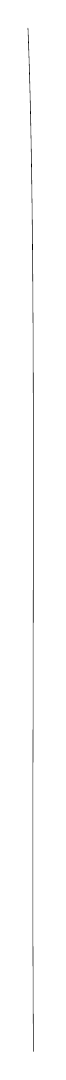
\begin{tikzpicture}[x=1cm,y=1cm]\draw[very thin] (0,0)..controls (.12,-3) and (.04,-9)..(.07,-13);\end{tikzpicture}}}
Or $\overline U$ est fortement 1-acyclique pour $\mathbb L$, donc $H^1(\overline U,\overline g^*\overline F)=0$ et $H^0(\overline U,\overline g^*\overline F)\simeq H^0(\widetilde S,\widetilde F)$. Par suite on a des isomorphismes (``suite spectrale de Hochschild-sSerre en bas dimensions'')
\[
H^1(G,H^0(\widetilde S,\widetilde F))\simeq H^1(\widetilde U,\widetilde g^*\widetilde F)\simeq((R^1j_*)g^*F)_{\overline x},
\]
où $G=\varprojlim_n\mathbb Z/n\mathbb Z=\deleted{\unsure{G(\overline U/U)\ G(\widetilde U/U)}}\ G(\overline U/\widetilde U)$. Puisque $H^0(\widetilde S,\widetilde F)$ \deleted{commutent} et $G$ commutent trivialement au changement de base $\overline s\longrightarrow S$, il en est de même de $(R^1j_*)g^*F$.

Supposons enfin que $F$ soit un faisceau de \deleted{\unsure{$\mathbb L$}} $\mathbb L$-torsion. On va démontrer le théorème sous la forme
\diagram{\[
\begin{tikzcd}
{u'}^*(R^qi^!)g^*F\arrow[r,"\sim"]&(R^q{i'}^!){g'}^*u^*F
\end{tikzcd}
\]}
pour chaque $q$. Puisque le résultat est déjà démontrée pour $q=2$, il est évident de l'argument de recurrence dans la démonstration de (3.7) \deleted{\unsure{qui}} qu'il est \deleted{déjà} également vrai pour $q$ arbitraire dans le cas $F=\mathbb Z/n$ ($n$ premier aux caractéristiques résiduelles). Tenant compte de (VIII.5.5), on termine avec le lemme suivant:
\scanpage{69}
qui correspond donc à un isom
\[
\boxed{Q^\sigma\simeq Q}
\]
\mspage{68}
\scanpage{70}
\mspage{69}
\mspage{28}
\margin{démonstration peu \unsure{naturelle}\ \unsure{\P}}
\margin{\figure{\begin{tikzpicture}[x=1cm,y=1cm]\draw (.2,0)--(0,0)--(0,-.8)--(.15,-.8);\draw[very thin] (-.8,-.7)..controls (-.9,-1.6) and (-.85,-2.7)..(-.85,-3.5);\end{tikzpicture}}}
Démonstration. La première assertion veut naturellement dire que pour $S'\xrightarrow{u}S$ arbitraire, le morphisme
\diagram{\[
\begin{tikzcd}
{u'}^*(R^qj_*)g^*F\arrow[r]&(R^qj'_*){g'}^*u^*F
\end{tikzcd}
\]}
est bijectif dans les situations envisagées, où $u'=u\times_S X$, et la dernière assertion équivaut à la première pour les faisceaux abeliens (IV4.5.).

Pour $q=0$, on a (3.2) des isomorphismes
\diagram{\[
\begin{tikzcd}[row sep=large]
{u'}^*f^*F\arrow[r,"\sim"]\arrow[d,phantom,"{\rotatebox{90}{$\simeq$}}" description]&{u'}^*j_*g^*F\\
{f'}^*u^*F\arrow[r,"\sim"]&j'_*{g'}^*u^*F
\end{tikzcd}
\]}
d'où le résultat.

\margin{\figure{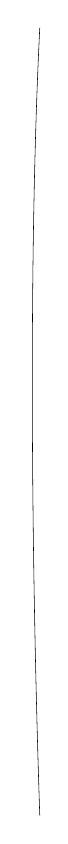
\begin{tikzpicture}[x=1cm,y=1cm]\draw[very thin] (0,0)..controls (-.15,-3) and (-.1,-7)..(0,-10);\end{tikzpicture}}}
Pour $q>0$, on se réduit comme d'habitude au cas $S,X,Y$ de type fini sur $\operatorname{Spec}\mathbb Z$. De plus, il suffit \deleted{\unsure{x}} évidemment de traiter le cas ou $S'=\overline s$ est un point \deleted{\unsure{geo}} géométrique de $S$ (cf. XII.6.5).
\margin{!}
Supposons que $F$ soit un faisceau de \deleted{groupes} ind $\mathbb L$-groupes. Si la codimension de $(Y,X)$ n'est pas 1 \deleted{\unsure{,}} (nous le supposons constant), on a $(R^qj_*)g^*=(R^qj'_*){g'}^*=0$ (3.4), d'où le résultat. Supposons que la codimension soit 1, et soit $\overline x$ un point géométrique de $X$ au dessus de $\overline s$ tel que son image soit dans $Y$. Reprenons les \deleted{\unsure{no}} notations de la démonstration de (3.5): on a
\scanpage{71}
Structures sur catégorie \inserted{$(C)$} de \inserted{\unsure{(gr)}} motifs ($1/2$ \unsure{simples}) sur un ouvert $S\subset\operatorname{Spec}(\mathbb Z)$.

\margin{\figure{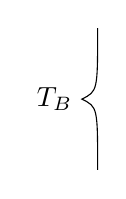
\begin{tikzpicture}[x=.2cm,y=.2cm]
\draw (1,9) .. controls (1,5) and (1,5) .. (0,4.5) .. controls (1,4) and (1,4) .. (1,0);
\node[left] at (0,4.5) {$T_B$};
\end{tikzpicture}}}
$T_B$ : foncteur de Betti (sur $\mathbb Q$) relatif : $\mathbb C$, \fbox{groupe $G$ sur $\mathbb Q$}
\[
T_\ell\simeq T_B\otimes_{\mathbb Q}\mathbb Q_\ell,
\qquad\text{réalisation $\ell$-adique (sur $\overline{\mathbb Q}\subset\mathbb C$)}
\]
\diagram{\begin{tikzcd}[column sep=small]
&\boxed{\begin{gathered}\begin{tikzcd}[column sep=small]
\pi=\operatorname{Gal}(\overline{\mathbb Q}/\mathbb Q)\arrow[r]&G(\mathbb Q_p)\\
\pi(p)=\operatorname{Gal}(\overline{\mathbb Q}_p/\mathbb Q_p)\arrow[u]&
\end{tikzcd}\end{gathered}}\arrow[r,bend left=20,no head]&\text{non ramifié dans }S-\{p\}\\
\pi(\infty)=\mathbb Z/2\mathbb Z\arrow[ur,bend left=20]& &p\in S\quad\text{($p$ premier fini ou $\infty$)}\arrow[ul,bend left=20,no head]
\end{tikzcd}}
\margin{\unsure{réalité} des autres \unsure{structures} $\unsure{\varphi^\infty|\mathbb C^\infty}$ resp \dots}
\[
\boxed{\begin{gathered}
\diagram{\begin{tikzcd}[column sep=large]
i_1^{(\infty)}\deleted{(\infty)},\ i_2^{(\infty)}\deleted{(\infty)}:\mathbb G_{m\mathbb C}\arrow[r,shift left]\arrow[r,shift right]&G(\mathbb C)\\
i_1^{(p)}\deleted{(p)},\ i_2^{(p)}\deleted{(p)}:\mathbb G_{m,\mathbb C^{(p)}}\deleted{\unsure{p}}\arrow[r,shift left]\arrow[r,shift right]&G(\mathbb C^{(p)})
\end{tikzcd}}
\end{gathered}}
\qquad\text{d'où}\quad
\left\{\begin{array}{l}
U^{(p)}\subset G_{\mathbb C^{(p)}}\\
U^{(\infty)}\subset G_{\mathbb C}\\
\text{(via }i_2^{(p)},i_2^{(\infty)}\text{)}
\end{array}\right.
\]
\figure{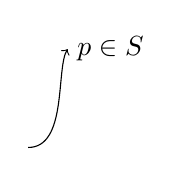
\begin{tikzpicture}[x=.5cm,y=.5cm]
\draw[->] (0,0) .. controls (1,0) and (.7,2) .. (1,2.5);
\node[right] at (1,2.5) {$p\in S$};
\end{tikzpicture}}

\margin{\figure{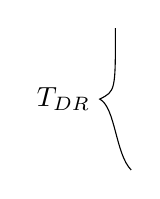
\begin{tikzpicture}[x=.2cm,y=.2cm]
\draw (1,9) .. controls (1,5) and (1,5) .. (0,4.5) .. controls (1,4) and (1,1) .. (2,0);
\node[left] at (0,4.5) {$T_{DR}$};
\end{tikzpicture}}}
$T_{DR}$ : foncteur de DeRham (sur $\mathbb Q$)

correspond à \fbox{torseur $P$ sous $G$}, groupe $G'$ sur $\mathbb Q$, $G'=\operatorname{ad}(P)=G^P$.

\uline{filtré}, i.e. on a une famille d'hom
\diagram{\begin{tikzcd}j_2:\mathbb G_{m\mathbb Q}\arrow[r,no head]&G'\end{tikzcd}}
défini mod conjugaison par les elts du groupe unipotent associé $U'\subset G'$ ($\Rightarrow$ torseur $R$ sur $U'$).

$\forall p\in S$, $p$ premier fini, on a
\[
\boxed{\begin{array}{l}F_p\in G'(\mathbb Q_p)\\F_\infty\in G'(\mathbb R)\end{array}}
\quad\text{(Frobenius)}
\]
\inserted{d'ordre $2$}

\margin{\figure{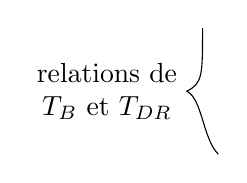
\begin{tikzpicture}[x=.2cm,y=.2cm]
\draw (1,8) .. controls (1,5) and (1,4.5) .. (0,4) .. controls (1,3.5) and (1,1) .. (2,0);
\node[left,align=center] at (0,4) {relations de\\$T_B$ et $T_{DR}$};
\end{tikzpicture}}}
\deleted{Etant \unsure{donné}} \deleted{$\unsure{\rho}$}
\[
\boxed{\rho^{(\infty)}\in P(\mathbb C)}
\]
transformant la classe des $\unsure{j'_{2\mathbb C}|j_{2\mathbb C}}$ en celle de $i_2^{(\infty)}$.

Pour tt $\unsure{j_2^*|j'_2}\in U'$, et tout $\lambda\in\mathbb C^p(1)^*$, on obtient
\[
\boxed{\rho^{(p)}(j_2,\lambda)\in P(\mathbb C^p)}
\]
transformant le \uuline{$j_2$ en $i_2$}

i.e.
\[
\left\{\begin{gathered}
\diagram{\begin{tikzcd}
\mathbb C^{(p)}(1)^*\times U'(\unsure{\mathbb C^p|\mathbb C})\arrow[r,no head]&P(\mathbb C^p)
\end{tikzcd}}\\
\boxed{\begin{gathered}\diagram{\begin{tikzcd}
\mathbb G_{m\mathbb C^p}\arrow[r,"i_2^{(p)}"]&\unsure{G_{\mathbb C^p}|G'_{\mathbb C^p}}&G'_{\mathbb C^p}\supset U'_{\mathbb C^p}
\end{tikzcd}}\end{gathered}}
\end{gathered}\right.
\]
et compatibilité aux opérations de

\begin{tabular}{ll}
a)&$\mathbb C^{(p)*}\times U'(\mathbb C^p)$\\
b)&$\pi(p)=\operatorname{Gal}(\overline{\mathbb Q}_p/\mathbb Q_p)$
\end{tabular}
\mspage{70}
\scanpage{72}
\mspage{71}
\begin{center}- 35 -\end{center}
\begin{flushright}n°357\end{flushright}
nous énonçons sous forme de Lemme :

LEMME 3.- \uline{Soient} $\lambda$, $\lambda'$ \uline{deux mesures composables sur} $G$ ; \uline{soit} $\psi$ \uline{un caractère (représentation continue) de} $G$ \uline{dans} $\mathbb C^*$ ; \uline{alors} $\psi,\lambda$ \uline{et} $\psi.\lambda'$ \uline{sont composables, et on a} :
\[
(\psi.\lambda)*(\psi.\lambda')=\psi.(\lambda*\lambda').
\]
On peut exprimer les résultats ci-dessus en disant que, par la loi $(\lambda,f)\to(\chi^{1/q}.\lambda)*f$, l'algèbre $\mathcal M_b^1(G)$ opère continument sur $L^p(E;\gamma)$.

PROPOSITION 9.- \uline{Soient} $\lambda$ \uline{une mesure bornée sur} $G$, $f\in\mathcal L^p$, $g\in\mathcal L^q$ ; \uline{alors on a} :
\[
\tag{14}
\int g.(\chi^{1/q}\lambda*f)\,d\gamma
=\int(\chi^{1/p}\lambda^\vee*g).f\,d\gamma,
\]
\uline{où} $\lambda^\vee$ \uline{est la mesure donnée par} $d\lambda^\vee(x)=d\lambda(x^{-1})$, \uline{c'est-à-dire l'image de} $\lambda$ \uline{par} $x\to x^{-1}$.

Observons d'abord qu'on a, pour $F\in\mathcal K(E)$ :
\[
\begin{aligned}
\int F(xz)\chi(x)^{1/q}\,d\lambda(x)
&=\int F(x^{-1}z)\chi(x)^{-1/q}\,d\lambda^\vee(x)=\\
&=\int F(x^{-1}z)\chi(x)^{1/p}.\chi(x^{-1})\,d\lambda^\vee(x)
=\int((\unsure{\chi|\lambda}^{1/p}\lambda^\vee)*F)(z).
\end{aligned}
\]
Dans ces conditions, si on applique au premier membre de la formule (2), dans la prop.2, le théorème de Lebesgue-Fubini, après y avoir remplacé $\mu$ par $\chi^{1/q}\lambda$, on obtient (14) avec $F$ au lieu de $g$ ; cela démontre (14) pour $g\in\mathcal K(E)$. Comme les deux membres dépendent continument de $g\in\mathcal L^p$ en vertu de la prop.8, et que $\mathcal K(E)$ est partout dense dans $\mathcal L^p$, la conclusion s'ensuit.

[Le rédacteur (resp. le lecteur) s'aperçoit avec plaisir (resp. chagrin) que la belle Prop.6 de la rédaction antérieure, (p.57), avec ses succulentes conditions $\mathrm{DM}_{\mathrm I}$, $\mathrm{DM}_{\mathrm {II}}$, $\mathrm{DM}_{\mathrm {III}}$, $\mathrm{DM}_{\mathrm {IV}}$, dont Bourbaki semblait si fier,a disparu sans laisser de trace, vu qu'il n'en a eu nul besoin pour la convolution dans les $L^p$, non plus que du n° hérétique du §1, ni de l'intégration vectorielle, ni des hypocons, etc. Tremblant de crainte à l'idée de déplaire à son illus-
\scanpage{73}
\diagram{\begin{tikzcd}
\mathbb Q&\mathbb C\\
H_B^*(X_{\mathbb C})\arrow[r,"\text{oui}",no head]&H_B^*(X)\otimes_{\mathbb Q}\mathbb C
\end{tikzcd}}
\margin{$\mathbb Q$}
\deleted{\uuline{bigradué} \uline{$\unsure{\pi|m.}$}}
\figure{\begin{tikzpicture}
\node[draw,ellipse,align=left] at (0,0) {oui\\\unsure{mais tordu}};
\draw (-1,-.4)--(-.7,.4);
\node[draw,ellipse] at (3,0) {\uuline{non}?};
\draw (2.4,.4)--(2.7,-.4);
\end{tikzpicture}}
\diagram{\begin{tikzcd}[column sep=small]
\unsure{L|K}&\deleted{H_{Hdg}(X)}\arrow[dr,no head]&H_{DR}\arrow[d,no head]&\unsure{L|K}\\
&&H_{\mathrm{cris}}&
\end{tikzcd}}
\diagram{\begin{tikzcd}[column sep=small]
H^{\unsure{r|\nu}}(X,\mathcal O_X)\arrow[r,no head]&H^{\unsure{r-1|\nu-1}}(X,\Omega_X^1)\arrow[r,no head]\arrow[d,no head]&{}\\
&{}\arrow[r,no head]&H_{\mathrm{cris}}
\end{tikzcd}}
\deleted{$\unsure{H^r|H^\nu}(X,\mathcal O_X$}

$i_1$

\deleted{$H_{DR}(X)\otimes_{\mathbb R}\mathbb C\simeq H(X_{\mathbb C},\mathbb R)\otimes_{\mathbb R}\mathbb C$}
\deleted{\diagram{\begin{tikzcd}H_{DR}^*(X_L)\arrow[r,no head]&H_{DR}^{\unsure{*|1}}(X_{\mathbb C})\end{tikzcd}}}
\deleted{$\sigma_1.\sigma_2=f$}
\inserted{\unsure{autom.} \unsure{galois}}
\[
Q^\sigma\simeq Q
\]
\diagram{\begin{tikzcd}X_{\mathbb R}\arrow[r,no head]&X_{\mathbb C}\end{tikzcd}}
\[
H^*(X(\mathbb C),\mathbb C)
\]
\deleted{$H^*(X$}
\[
G
\]
\figure{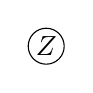
\begin{tikzpicture}\node[draw,circle,inner sep=1pt] {$\unsure{\mathbb Z}$};\end{tikzpicture}}
\[
S\subset\operatorname{Spec}(\mathbb Z)
\]
\deleted{\diagram{\(\begin{array}{c@{\quad}c}
\left\{\begin{array}{c}\boxed{\begin{array}{c}T_B\\T_{DR}\end{array}}\\T_{Hdg}\end{array}\right.&\begin{array}{ll}:&G_B\\:&G_{DR}\\&\end{array}
\end{array}\)}}
\margin{\deleted{\diagram{\begin{tikzcd}\unsure{S}\arrow[d,no head,"\unsure{lisse}"]\\\operatorname{Spec}\mathbb Z\end{tikzcd}}}}
\margin{\figure{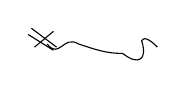
\begin{tikzpicture}[x=.4cm,y=.4cm]
\draw (0,2)--(.8,1.5);\draw (.1,2.2)--(.9,1.6);\draw (.2,1.6)--(.8,2.1);
\draw (.6,1.7) .. controls (1,1.2) and (1.1,2) .. (1.6,1.7) .. controls (2.2,1.5) and (2.5,1.4) .. (3,1.4) .. controls (3.5,1) and (3.8,1.2) .. (3.6,1.8) .. controls (3.7,2) and (4,1.7) .. (4.1,1.6);
\end{tikzpicture}}}

a) $M$ \unsure{module} à conn. intégrable \inserted{sur $S$}, avec \uline{filtration}.

b) \diagram{\begin{tikzcd}M(p)^\sigma\arrow[r,"F_p"]&M(p)\end{tikzcd}} Frobenius \deleted{\unsure{au}} (hom de cristaux)

c) $\mathbf M(\mathbb R)$ fibré \inserted{analytique \deleted{\unsure{filtré}}} (sur $S(\mathbb R)$), muni d'un autom. $F_\infty$ d'ordre $2$.

d) \deleted{$\unsure{B}$} $T$ (betti) système local sur $S_{\mathbb C}^{\deleted{\unsure{*}}\mathrm{an}}$ ($\Rightarrow\pi_1(S_{\mathbb C}^{\mathrm{an}},s)\to\operatorname{Aut}(T_s)$)

e) $T_p$ syst. local sur $S-S_p$ \qquad $T_p\simeq T\otimes_{\mathbb Z}\mathbb Z_p$ sur $S_{\mathbb C}$

$\unsure{f_\infty)}$ $M_{\mathbb C}^{\mathrm{an}}\simeq T\otimes_{\mathbb Z}\mathbb C$

$f_p)$ \qquad $-\ -\ -\ -\ -$
\mspage{72}
\scanpage{74}
\mspage{73}
\begin{flushright}31\end{flushright}
Soit $(Y,X)$ un $S$ -couple lisse de codimension $1$, et supposons que $Y$ soit défini dans $X$ par une équation $t=0$. Notons aussi par $t$ la section inversible de $\Gamma(U,\mathcal O_U)$ obtenu par restriction (notation de (3.1)). De la suite exacte de Kummer (IX.3.2) sur $U$
\diagram{\begin{tikzcd}0\arrow[r]&\mu_n\arrow[r]&\mathbb G_m\arrow[r,"n"]&\mathbb G_m\arrow[r]&0\end{tikzcd}}
on déduit un morphisme ``cobord''
\diagram{\begin{tikzcd}j_*\mathbb G_m\arrow[r,"\delta"]&R^1j_*\mu_n\end{tikzcd}}
d'où une section $\delta t$ de $R^1j_*\mu_n$. Puisque $n$ est annihilateur de $R^1j_*\mu_n$, cette section donne un morphisme
\[
\tag{3.9}
\varepsilon_t:(\mathbb Z/n)_Y\longrightarrow(R^2i^!)(\mathbb Z/n)_X\approx i^*(R^1j_*)(\mathbb Z/n)_U.
\]
Nous verrons que $\varepsilon_t$ est un bijection canonique.

\uline{Théorème(3.10):} Soit $C$ La famille des couples lisses de codimension constant. Il existe un fonction et un seul $\varphi$ donnant pour chaque $S$ -couple lisse $(Y,X)$ de codimension $c$ \inserted{et chaque $n$ premier aux caractéristiques résiduelles de $X$} un isomorphisme (dit canonique) de faisceaux
\deleted{\diagram{\begin{tikzcd}
(\unsure{Y|U},X)\ -\ :\ \mathbb Z/n\arrow[r]&\underline H_Y^{2c}(X,\unsure{\gamma|\mathbb Z}^{\unsure{u|n}}
\end{tikzcd}}}
\scanpage{75}
Conj. de Hodge (simple, généralisée)
\margin{déc. de Hodge sur $\mathbb C$}

Conj. de Tate (simple, généralisée)
\margin{opération de Galois, resp. Frobenius}

Conj. des Frobenius dans Ch. de De Rham (à connexion)
\margin{Frobenius \unsure{cristallin|cristallins}}

\margin{?}
Conj. \unsure{du|des} double réseau (revoir)

``Tate \unsure{grou|group}'' (simple, \unsure{généralisé}) sur schém.
\diagram{\(\begin{array}{l}
\left\{\begin{array}{l}\text{de t.f. sur }\mathbb Z\\\text{de t.f. sur corps}\end{array}\right.
\end{array}\)}

``Tate \unsure{grou|group}'' sur anneau local d'inégale car.
\mspage{74}
\scanpage{76}
\mspage{75}
\begin{center}- 33 -\end{center}
\begin{flushright}n°357\end{flushright}
\[
\varepsilon_x*f-\varepsilon_{x_0}*f_0
=\varepsilon_x*(f-f_1)-\varepsilon_{x_0}*(f_0-f_1)+(\varepsilon_x-\varepsilon_{x_0})*f_1
\]
et par suite, si $N_p(f-f_0)\leq\delta$ et $x\in\unsure{K|\mathcal K}$ :
\[
N_p(\varepsilon_x*f-\varepsilon_{x_0}*f_0)\leq3C\delta+N_p((\varepsilon_x-\varepsilon_{x_0})*f_1)
\]
où on a posé $C=\sup_K(\chi^{-1/q})$. Mais on a :
\[
N_p((\varepsilon_x-\varepsilon_{x_0})*f_1)^p
=\int\left|f_1(x^{-1}z)\chi(x^{-1})-f_1(x_0^{-1}z)\chi(x_0^{-1})\right|^p\,d\gamma(z)\ ;
\]
si $K_1$ est le support de $f_1$, la fonction $f_1(x^{-1}z)\chi(x^{-1})$ induit sur $K\times E$ une fonction continue dont le support est contenu dans $K\times(K.K_1)$ ; celle-ci est donc uniformément continue ; on en conclut aussitôt qu'il existe un voisinage $V$ de $x_0$ dans $K$ tel que le second membre de la relation ci-dessus soit $\leq\delta$ pour $x\in V$. Cela achève la démonstration.

\uline{Remarque} 1.- Le formule (10) reste évidemment valable pour $p=+\infty$ ; la démonstration ci-dessus montre alors que $(x,f)\to\varepsilon_x*f$ est une application continue de $G\times\overline{\mathcal K(E)}$ dans $\overline{\mathcal K(E)}$.

\uline{Remarque} 2.- Comme $\varepsilon_x*f$ est négligeable si $f$ l'est [N.B. - Pour le style, cf. ``puisque mon époux l'est'', P. Corneille, \uline{Horace}, \unsure{1e|le} éd., Acte I, Sc. 1], l'application $(x,f)\to\varepsilon_x*f$ détermine, par passage au quotient, une application de $G\times L^p$ dans $L^p$, qu'on note aussi $(x,f)\to\varepsilon_x*f$, et qui satisfait aussi à (10). Une remarque analogue s'applique aux opérations définies ci-dessous.

PROPOSITION 8.- \uline{Soit} $\lambda$ \uline{une mesure bornée sur} $G$ ; \uline{pour} $1\leq p<+\infty$, \uline{soit} $\mu=\chi^{1/q}.\lambda$, \uline{et soit} $f\in\mathcal L^p(E,\gamma)$. \uline{Alors} $\mu$ \uline{et} $f$ \uline{sont composables, et on a}
\[
\tag{11}
N_p((\chi^{1/q}.\lambda)*f)\leq N_p(f).\lVert\lambda\rVert.
\]
Le lemme 2 du n°2 montre que le support de $\lambda$, donc celui de $\mu$, est réunion dénombrable de compacts ; on peut donc appliquer la prop.6 du n°2, où l'on a, d'après la prop.7 et l'inégalité de Hölder :
\scanpage{78}
\uline{Complexe de \unsure{cotie} des groupes de \unsure{t.m.}.}

1. Soit $G=D(M)$, $M$ un réseau sur $S$ = \unsure{grpe|groupe} ct tordu sur $S$.

Considérons la résolution plate canonique en deux crans
\[
\tag{1.1}
\diagram{\begin{tikzcd}0\arrow[r]&R\arrow[r,"v"]&\mathbb Z[M]\arrow[r,"u"]&M\arrow[r]&0\end{tikzcd}},
\]
\unsure{où} $R=\operatorname{Ker}u$, $u([m])=m$. On en déduit, par passage aux duals, une suite exacte
\[
\tag{1.2}
\diagram{\begin{tikzcd}
0\arrow[r]&G\arrow[r,no head]&T\arrow[r,no head]\arrow[d,equal]&T'\arrow[r,no head]\arrow[d,equal]&0\\
&&\mathbb G_m^M&D(R)&
\end{tikzcd}}
\]
résolvant $G$ par des tores. (\unsure{évt} de dim. relative infinie\dots).

Le triangle de transitivité de \unsure{Mazur-Roberts} donne un isomorphisme
\deleted{$\unsure{\ell_G|L_G}$}
\[
\ell_\bullet^G\simeq
\left[\diagram{\begin{tikzcd}\omega_{T'}\arrow[r,no head]&\omega_T\end{tikzcd}}\right]
\simeq\left[\diagram{\begin{tikzcd}R\otimes_{\mathbb Z}\mathcal O_S\arrow[r]&\mathbb Z[M]\otimes_{\mathbb Z}\unsure{\mathcal O_S}\end{tikzcd}}\right.
\]
i.e.
\[
\tag{1.3}
\boxed{\ell_\bullet^G\simeq\underline M\overset{\mathbf L}{\otimes}_{\mathbb Z}\underline{\mathcal O}_S}
\]
\figure{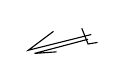
\begin{tikzpicture}[x=.4cm,y=.4cm]
\draw (2,.5)--(0,0)--(.8,.6);\draw (1.9,.35)--(.2,-.1)--(.9,-.05);
\draw (1.7,.7)--(1.9,.2)--(2.2,.25);
\end{tikzpicture}}
Si \deleted{\unsure{on}} $\mathcal O_S$ est \unsure{une} $\Lambda$-Algèbre (p.ex. $\Lambda=\mathbb Q$, ou $\Lambda=\mathbb Z/n\mathbb Z$)

\deleted{$n\mathcal O_S=0$, i.e. $\mathcal O_S$ une $\mathbb Z/n\mathbb Z$-Algèbre,}

on peut écrire aussi
\[
\tag{1.4}
\boxed{\ell_\bullet^G\simeq
\bigl(M\overset{\mathbf L}{\otimes}_{\mathbb Z}\Lambda\deleted{\unsure{\mathbb Z/n\mathbb Z}}\bigr)
\overset{\mathbf L}{\otimes}_{\Lambda\deleted{\unsure{\mathbb Z/n\mathbb Z}}}\mathcal O_S}
\]
et si
\mspage{77}
